%**************************************************************************************************
%*  Nome: Nicolas P. Lane                                                                         *
%*  Data: 13/10/2015                                                                              *
%*  D�vidas ou contribui��es: lambdox@gmail.com                                                   *
%*  Modelo de monografia para TCC - UDESC de acordo com o manual de trabalhos acad�micos da UDESC *                                     *
%*  									                          *
%*  Licen�a GPL:              						                          *
%*  Permission to use, copy, modify, and distribute this protocol and its                         *
%*  documentation for any purpose, without fee, and without written                               *
%*  agreement is hereby granted, provided that the above copyright notice,                        *
%*  and the author appear in all copies of this protocol.                                         *
%**************************************************************************************************

\NeedsTeXFormat{LaTeX2e}
%-----------------------------------------------------------
\documentclass[a4paper,12pt]{monografia}
\usepackage{amsmath, amsthm, amsfonts, amssymb}
\usepackage[english, brazilian]{babel}
\usepackage[titletoc]{appendix}
\usepackage[latin1]{inputenc}
\usepackage[mathcal]{eucal}
\usepackage[alf]{abntcite}
\usepackage{subfigure}
\usepackage{isoaccent}
\usepackage{textcase}
\usepackage{multirow}
\usepackage{latexsym}
\usepackage{graphicx}
\usepackage{listings}
\usepackage{acronym}
\usepackage{bm}
\lstset{basicstyle=\tiny, language=C++}
\makeindex			
%-----------------------------------------------------------Come�a documento
\begin{document}
%----------------- T�tulo e Dados do Autor -----------------
\titulo{Seu t\'itulo}
\autor{Seu nome}
\nome{Seu nome do meio}
\ultimonome{Seu \'ultimo nome}

%---------- Informe o Curso e Grau -----
\bacharelado \curso{Ci\^encia da Computa\c{c}\~ao} \mes{Junho} \ano{2015} 
\data{\today} % data da aprova��o
\cidade{Joinville}

%----------Informa��es sobre a Institu��o -----------------
\instituicao{Universidade do Estado de Santa Catarina}
\sigla{UDESC} \unidadeacademica{Centro de Ci\^encias Tecnol\'ogicas}

%------Nomes do Orientador, 1o. Examinador e 2o. Examinador-
\orientador{Nome completo do orientador 1}
\examinadorum{Nome completo do orientador 2}
\examinadordois{Nome completo do orientador 3}
%\examinadorquatro{Nome do Examinador 4}

%--------- T�tulos do Orientador 1o. e 2o. Examinadores ----
\ttorientador{T\'itulo do orientador 1}
\ttexaminadorum{T\'itulo do orientador 2}
\ttexaminadordois{T\'itulo do orientador 3}
%\ttexaminadorquatro{T�tulo do Examinador 4}

\maketitle
%---------------------- AGRADECIMENTO --------------
\agradecimento{Agradecimentos}

  AAAAAAAAAAAAAAAAAAAAAAAAAAAAAAAAAAAAAAAAAAAAAA AAAAAAAAAAAAAAAAAAAAAAAAAAAAAAAAAAA AAAAAAAAAAAAAAAAAAAAAAAAAAAAAAAAAAAAAAAAAAAAAA 
AAAAAAAAAAAAAAAAAAAAAAAAAAAAAAAAAAA AAAAAAAAAAAAAAAAAAAAAAAAAAAAAAAAAAAAAAAAAAAAAA AAAAAAAAAAAAAAAAAAAAAAAAAAAAAAAAAAA 
AAAAAAAAAAAAAAAAAAAAAAAAAAAAAAAAAAAAAAAAAAAAAA AAAAAAAAAAAAAAAAAAAAAAAAAAAAAAAAAAAAAAAAAAAAAA AAAAAAAAAAAAAAAAAAAAAAAAAAAAAAAAAAA 
AAAAAAAAAAAAAAAAAAAAAAAAAAAAAAAAAAA

\newpage
%---------------------- EP�GRAFE --------------
\begin{epigrafe}

  Disce Docendo Adhuc

\end{epigrafe}
%--------Digite aqui o seu resumo em Portugu�s--------------
\resumo{Resumo}
\begin{resumo}

\begin{center}
 Resumo do Trabalho de Conclus�o de Curso apresentado � UDESC como parte dos requisitos necess�rios para obten��o do grau de Cientista da Computa��o.


{% Norma - fonte negrito, corpo 16
\bfseries
\LARGE

\ABNTtitulodata

}

\end{center}


\begin{singlespace}
	\noindent Orientador: \ABNTorientadordata\ \\
	\noindent Co-orientador: \ABNTcoorientadordata\ \\ %comentar sen�o tiver co-orientador
  \noindent Palavras-chave: Escreva; Aqui; Suas; Palavras-chave\\
\end{singlespace}


Escreva aqui o texto de seu resumo...




\end{resumo}


%chamada de arquivo resumo.tex

\noindent Palavras-chaves: Comunica��o Alternativa, Paralisia Cerebral, defici�ncia na fala, software livre
%-----------Digite aqui o seu resumo em Ingl�s--------------
\resumo{Abstract}
\begin{abstract}

\begin{center}

Abstract of bachelor monograph presented to UDESC as a partial fulfillment of the requirements for the degree of Computer Engineering.

{% Norma - fonte negrito, corpo 16
\bfseries
\LARGE

Title

}

\end{center}

\begin{singlespace}
  \noindent Advisor: \ABNTorientadordata \\
  \noindent Co-advisor: \ABNTcoorientadordata\\ %comentar sen�o tiver co-orientador
  \noindent Key words: Write; Here; Your; Key-words.\\
\end{singlespace}


Write here the English version of your `Resumo'...

\end{abstract}
     %chamada de arquivo abstract.tex

\noindent Keywords: Alternative Comunication, Cerebral Palsy, speech deficiency, open source
%-----------------------------------------------------------

\listoffigures       %gera p�gina com lista de figuras a partir de todas as entradas feitas no documento

% lista de abrevia��es
\listoftables        %gera p�gina com lista de tabelas a partir de todas as entradas feitas no documento
\chapter*{Lista de Siglas e Abreviaturas}
\addcontentsline{toc}{chapter}{Lista de Siglas e Abreviaturas}
\begin{acronym}

\acro{ACE}[ACE]{Associa��o Catarinense de Ensino}
\acro{ADA}[ADA]{\textit{Americans with Disabilities Act}}
\acro{ADEJ}[ADEJ]{Associa��o dos Deficientes F�sicos de Joinville}
\acro{APAE}[APAE]{Associa��o de Pais e Amigos dos Excepcionais de Joinville}
\acro{APCB}[APCB]{Associa��o de Paralisia Cerebral do Brasil}
\acro{APIS}[APIs]{\textit{Application Programming Interfaces}}
\acro{ARASSAC}[ARASSAC]{Portal Aragon�s de Comunica��o Alternativa e Ampliada}
\acro{ARCD}[ARCD]{Associa��o de Reabilita��o da Crian�a Deficiente}
\acro{CA}[CA]{Comunica��o Alternativa}
\acro{CAA}[CAA]{Comunica��o Alternativa e Ampliada}
\acro{CAT}[CAT/SEDH]{Comit� de Ajudas T�cnicas da Secretaria de Direitos Humanos}
\acro{eMAG}[eMAG]{Modelo de Acessibilidade de Governo Eletr�nico}
\acro{EUSTAT}[EUSTAT]{\textit{Empowering Users Through Assistive Technology}}
\acro{HEART}[HEART]{\textit{Horizontal European Activities in Rhabilitation Technology}}
\acro{JVM}[JVM]{\textit{Java Virtual Machine}}
\acro{ONU}[ONU]{Organiza��o das Na��es Unidas}
\acro{PC}[PC]{Paralisia Cerebral}
\acro{TA}[TA]{Tecnologia Assistiva}
\acro{UDESC}[UDESC]{Universidade do Estado de Santa Catarina}
\acro{W3C}[W3C]{World Wide Web Consortium}

\end{acronym}    %chamada de arquivo acronimos.tex

%----Sum�rio, lista de figura e de tabela ------------
\tableofcontents      %gera p�gina com sum�rio a partir de todas as entradas feitas no documento

%--------------In�cio do Conte�do---------------------------
\pagestyle{ruledheader} %estilo abnt2
\chapter{Introdu��o}
\label{cap:introducao1}


A acessibilidade � a possibilidade de qualquer pessoa, independentemente de suas capacidades f�sico-motoras e perceptivas, culturais e sociais, usufruir os benef�cios de uma vida. Al�m disso, a acessibilidade tem como objetivo possibilitar o acesso de pessoas com defici�ncia permanente ou tempor�ria (e.g., f�sicas, auditivas, etc.) na sociedade afim de que todas possam participar ativamente.

Para que o objetivo da acessibilidade seja cumprido, � necess�rio o estudo e cria��o de alternativas, para que estas pessoas possam contornar ou compensar algum tipo de defici�ncia que as impe�a a sua inser��o. Essa demanda motivou o surgimento da \acf{TA}, uma parte da tecnologia que deve ser entendida como um aux�lio que promove a amplia��o de uma habilidade funcional deficit�ria ou possibilitar a realiza��o da fun��o desejada e que se encontra impedida. Contudo, ainda s�o encontradas muitas dificuldades, principalmente pelo tema ser consideravelmente novo, a quantidade de trabalhos cient�ficos relacionado ao tema ainda � pouco expressivo.

Nas diferentes classifica��es da \ac{TA}, existe a \acf{CAA} que pode ser definida como uma alternativa a comunica��o escrita e oral. A \ac{CAA} inicialmente era composta apenas de sistemas sem tecnologia, como libras, cart�es e livros. Por�m, com o avan�o da tecnologia nas �ltimas d�cadas, sistemas anal�gicos e sistemas com recursos computacionais foram aumentando o escopo e as alternativas de \ac{CAA}.

Com uma quantidade expressiva de pessoas com algum tipo de paralisia no Brasil e no mundo, meios alternativos de inclus�o s�o necess�rios, principalmente meios alternativos dispon�veis a popula��o com baixa renda. Um dos objetivos espec�ficos do trabalho � analisar e diferenciar solu��es de \ac{CAA} que possibilitam a estimula��o cognitiva de pessoas com \acf{PC} em especial as pessoas que possuem habilidades locomotoras limitadas em conjunto com dificuldades na fala. Ap�s esta an�lise, verificar se � necess�ria a implementa��o de uma solu��o alternativa a essas pessoas. Contudo, esta s� pode ser atingida atrav�s de estudos sobre \ac{PC} e os requisitos que estas solu��es demandam. O principal objetivo do trabalho resume-se em implementar um software para computador alternativo de \ac{CAA} de licen�a GPL, para que pessoas com \ac{PC} possam ter seus c�rebros estimulados cognitivamente. 

A organiza��o deste trabalho est� dividida em quatro cap�tulos, ``Conceitos B�sicos'', ''Defini��o do Problema'', ``Proposta'' e ``Considera��es''. No primeiro cap�tulo s�o apresentados a quantidade de pessoas com defici�ncia no Brasil e no mundo, defini��es e legisla��o sobre \ac{TA} e \ac{TA} dentro da inform�tica, tamb�m � abordado as pessoas que possuem \ac{PC} e seus diferentes casos. Al�m disso, tamb�m estuda-se as principais iniciativas de \ac{TA} pelo mundo e seus termos e classifica��es. Ao final do cap�tulo � apresentado as defini��es de \ac{CAA} os seus recursos e estrat�gias e quais os termos e classifica��o que ser�o utilizados no trabalho.

No segundo cap�tulo, � definido o problema e os usu�rios finais da solu��o. O trabalho nesta parte levanta problemas com a prancha de comunica��o, que � a solu��o atual dos terapeutas, e ap�s isso identifica os requisitos necess�rios para o desenvolvimento da solu��o atrav�s de entrevista com uma psic�loga especialista em reabilita��o de pessoas com \ac{PC}. Ao final s�o identificados trabalhos correlatos e apresentado uma compara��o com base nos requisitos levantados.

No terceiro cap�tulo, � elaborado uma especifica��o da proposta, determinando os m�todos que ser�o utilizados para cumprir os requisitos levantados. Atrav�s de diagramas das tarefas, diagramas de classe e de estados da solu��o o trabalho indica quais ser�o as intera��es do usu�rio com a solu��o. S�o mencionados tamb�m os limitadores e e plano de teste que tem como objetivo fazer com que a solu��o evolua no decorrer do trabalho. 

\chapter{Conceitos}
\label{cap:introducao}
\acresetall
Ao longo da hist�ria em rela��o �s pessoas com defici�ncia, � poss�vel encontrar uma variedade de termos que foram se modificando ao longo dos anos: ``Inv�lidos'', ``incapacitados'', ``defeituosos'', ``excepcionais'' s�o alguns exemplos de termos atribu�dos �s pessoas com defici�ncia em diferentes �pocas. Os termos s�o considerados corretos em fun��o de valores e conceitos vigentes em cada sociedade e em cada �poca, portanto, os termos supracitados foram aceitos, usados e, em dados momentos da hist�ria, substitu�dos. No estudo da evolu��o do conceito da defici�ncia encontra-se que, em 1980, a Organiza��o Mundial de Sa�de prop�s a utiliza��o da CIDID - Classifica��o das Defici�ncias, Incapacidades e Desvantagens\cite{cidid} ({\it Handicaps})\footnote{Termo em ingl�s traduzido como defici�ncia} com intuito de organizar uma linguagem universal a respeito das defici�ncias. A implementa��o de uma nova terminologia, ``pessoas deficientes'', passou a atribuir o valor de pessoa a aqueles que at� ent�o eram desconsiderados como tais pela sociedade. Ressalta-se que a revis�o dessas nominatas teve a preocupa��o de centrar-se na pessoa e n�o na defici�ncia \cite{fiquene,chagas}.

Segundo a \citeonline{onu}, existem no mundo 1 bilh�o de pessoas que possuem algum tipo de defici�ncia. Segundo o Censo de 2010 \cite{censo} a ocorr�ncia de pessoas com defici�ncia na popula��o brasileira � de 23,9\% da popula��o. A tabela \ref{tabela_pop} apresenta a distribui��o dos tipos de defici�ncia no Brasil.


\begin{table}[bth!]
\centering
\scriptsize
\caption{Distribui��o dos tipos de defici�ncia no Brasil.}\vspace{.2cm}

	
    \begin{tabular}{ | l | l |}
		
    \hline
    Condi��o & Por��o da Popula��o\\ \hline \hline
    Defici�ncia Visual & 18,6\%\\ \hline
		Defici�ncia Motora & 7\%\\ \hline
		Defici�ncia Auditiva & 5,1\%\\ \hline
		Defici�ncia Mental ou Intelectual & 1,4\%\\ \hline
		
    \end{tabular}
    \label{tabela_pop}
		\vspace{0.1cm}\\Fonte: o pr�prio autor com base no Censo de 2010\cite{censo}.

\end{table}



A tabela \ref{tabela_pop} mostra que na popula��o brasileira, 18,6\% da popula��o possuem defici�ncia visual sendo a defici�ncia mais recorrente entre os brasileiros. A defici�ncia motora, a segunda com maior recorr�ncia, � apresentada em 7\% da popula��o, seguida da defici�ncia auditiva com 5,1\%, e das pessoas com defici�ncia mental que apresentam 1,4\%. Na tabela \ref{tabela_pop} a soma das porcentagens n�o � igual a 23,9\% pois algumas pessoas possuem mais de uma defici�ncia citada. Outro fator importante � que 65\% das pessoas que possuem algum tipo de defici�ncia recebem menos de dois sal�rios m�nimos no Brasil\cite{censo}, sendo que 10\% dessas pessoas tem renda de menos da metade de um sal�rio m�nimo. 

As pessoas que possuem algum tipo de defici�ncia sofrem dificuldades ao acesso das necessidades b�sicas conquistadas pelo ser humano, segundo o Programa de A��o Mundial para Pessoas Deficientes da ONU\cite[p.~11]{onu},

\begin{quotation}''[...] a experi�ncia tem demonstrado que, em grande medida, � o meio que determina o efeito de uma
incapacidade sobre a vida cotidiana da pessoa. A pessoa v�-se relegada � invalidez quando
lhe s�o negadas as oportunidades de que disp�e, em geral, a comunidade, e que s�o
necess�rias aos aspectos fundamentais da vida, inclusive a vida familiar, a educa��o, o
trabalho, a habita��o, a seguran�a econ�mica e pessoal, a participa��o em grupos sociais e
pol�ticos, as atividades religiosas, os relacionamentos afetivos e sexuais, o acesso �s
instala��es p�blicas, a liberdade de movimenta��o e o estilo geral da vida di�ria [...]''.
\end{quotation} 

Neste trabalho � dada �nfase a pessoas com defici�ncia motoras, mais especificamente as pessoas que possuem \ac{PC}.  A Encefalopatia Cr�nica da Inf�ncia (E.C.I.), tamb�m conhecida como \ac{PC}, � uma doen�a cr�nica de car�ter n�o evolutivo, que em 90\% das vezes possuem defici�ncia f�sica. O curso natural das les�es � de longa dura��o, necessitando a crian�a de tratamento prolongado. Tem efeitos n�o apenas sobre o crescimento e o desenvolvimento f�sico, mas tamb�m sobre a destreza, a personalidade, a capacidade cognitiva, as atitudes pessoais e sociais do paciente, as emo��es e as intera��es da fam�lia\cite{leite,sa}. Como a \ac{PC} possui diferentes tipos de manifesta��es e graus da doen�a, para maior compreendimento das necessidades de pessoas com \ac{PC}, � necess�rio conhecer os diferentes quadros cl�nicos da doen�a. 


\section{Quadro Cl�nico: \acf{PC}}

Existem v�rios quadros cl�nicos de pessoas, que possuem \ac{PC}, e podem ser beneficiadas por algum recurso que facilite a sua comunica��o com outras pessoas. Neste sentido alguns quadros se encaixam melhor ou pior a determinadas facilidades de comunica��o. As poss�veis causas da \ac{PC} (e.g., causas pr�-natais, perinatais e p�s-natais) n�o ser�o tratadas, pois n�o pertencem ao escopo deste trabalho.
Na observa��o cl�nica da \ac{PC}, deve-se levar em considera��o a extens�o do dist�rbio motor, sua intensidade e, principalmente, a caracteriza��o semiol�gica\footnote{Caracteriza��o semiol�gica, refere-se a caracteriza��o dos sinais e sintomas da doen�a.} desse dist�rbio\cite{leite}. Assim, a paralisia cerebral apresenta v�rias formas cl�nicas que s�o apresentadas na tabela \ref{tabela}.

\begin{table}[bth!]
\centering
\scriptsize
\caption{Tabela com os diferentes casos de \ac{PC}.}\vspace{.2cm}

	
    \begin{tabular}{ | l |  p{7cm} | p{5cm} |}
		
    \hline
    Quadro & Descri��o das Limita��es  & Aplic�vel recurso de comunica��o\\ \hline \hline
    Hemiplegia &   Sinais de libera��o tais como espasticidade , hiper reflexia e sinal de Babinski & Aplic�vel em alguns graus \\ \hline
    Hemiplegia bilateral & Tetra ou quadriplagia, dependendo do grau defici�ncia mental e epilepsia & Aplic�vel a pacientes com menor grau de les�o \\ \hline
    Diplegia & Com\-pro\-me\-ti\-men\-to dos membros inferiores, co\-mu\-men\-te evidenciando uma acentuada hipertonia dos adutores & Aplic�vel em alguns graus \\
    \hline
		Discinesia & Movimentos involunt�rios, ondulantes e repetidos com grande amplitude de movimento e incoordena��o motora &  Aplic�vel em alguns graus \\
    \hline
		Ataxia &  Perda de coordena��o dos movimentos musculares volunt�rios & Aplic�vel em alguns graus \\
    \hline
		Formas mistas & Combina��o dos quadros anteriores & Casos avaliados individualmente \\
    \hline
		
    \end{tabular}
    \label{tabela}
		Fonte: o pr�prio autor com base \citeonline{leite}.

\end{table}


A Tabela {\ref{tabela}} apresenta os diferentes quadros de \ac{PC}. Atrav�s dela pode-se perceber que independente do quadro, o grau da les�o de cada paciente com \ac{PC} tem que ser avaliado individualmente, para que se identifique quais s�o as necessidades de acessibilidade de cada um deles.  Para maiores informa��es sobre cada quadro cl�nico, ver Ap�ndice {\ref{apendice1}.



%No Brasil existem diversos movimentos sociais, dos mais variados �mbitos,voltados a ajudar as pessoas com defici�ncias. Tratando-se das pessoas com \ac{PC} os movimentos sociais tamb�m s�o decisivos. No entanto, os recursos normas e leis de acessibilidade ainda que claros, s�o parcialmente esquecidos pela sociedade e pela falta de investimento e pesquisa na �rea.As dificuldades encontradas s�o grandes, pois s�o poucas as literaturas especializadas e faltam equipamentos acess�veis a esse grupo da popula��o.

\section{Acessibilidade}

A acessibilidade � a possibilidade de qualquer pessoa, independentemente de suas capacidades f�sico-motoras e perceptivas, culturais e sociais, usufruir os benef�cios de uma vida em sociedade. � a possibilidade de participar de todas as atividades, at� as que incluem o uso de produtos, servi�os e informa��o, com o m�nimo de restri��es poss�vel \apud{nicholl,nbr}{unirio}.

As discuss�es sobre acessibilidade v�m crescendo no Brasil e no mundo \cite{donatangelo}.
O termo acessibilidade � muito amplo e, de certa forma, complexo de ser definido,
pois n�o pode ser entendido apenas como a facilidade de se ter acesso. Contudo, pode-se
caracterizar, de um modo geral, acessibilidade como sendo um processo din�mico que visa �
elimina��o de barreiras para que se tenha acesso.

A acessibilidade tamb�m � conhecida por ser a possibilidade e condi��o de alcance para a utiliza��o, com autonomia, simplicidade, efici�ncia e seguran�a, dos espa�os, mobili�rios, das edifica��es, dos equipamentos urbanos, dos transportes, dos sistemas e meios
de comunica��o e da inform�tica, por qualquer pessoa, sejam elas crian�as, adultos, idosos, contendo, ou n�o, necessidades especiais devido alguma defici�ncia ou mobilidade reduzida \apud{torres}{donatangelo}. No Brasil h� legisla��o que trata de quest�es de acessibilidade aos portadores de necessidades especiais. A legisla��o mais relevante no contexto deste trabalho s�o:
\begin{itemize}
\item Portaria n� 1.679, de dezembro de 1999, disp�e sobre requisitos de acessibilidade de 
pessoas portadoras de defici�ncias, para instruir os processos de autoriza��o e de 
reconhecimento de cursos, e de credenciamento de institui��es. 
 \cite{mec};
\item Lei n� 10.098, de dezembro de 2000, que, entre outras coisas, estabelece
normas gerais e crit�rios b�sicos para que seja promovida a acessibilidade
para pessoas com defici�ncia \cite{brasil}; e
\item Decreto n� 3.294, de dezembro de 1999, que instituiu o programa
Sociedade da Informa��o, na qual um dos objetivos � a universaliza��o do
acesso � Internet \cite{brasil1}.
\end{itemize}


Com a legisla��o presente, principalmente pelo decreto n� 3.294 a Acessibilidade ultrapassa as barreiras do espa�o f�sico e chega ao espa�o digital. No espa�o digital s�o encontradas muitas dificuldades, entre elas podem ser citadas a falta de
recursos tecnol�gicos, a falta de acesso aos recursos existentes e a falta de preocupa��o em
disponibilizar a informa��o de forma clara\apud{torres1}{donatangelo}. A utiliza��o de dispositivos eletr�nicos (e.g., computadores, {\it tablets} e { \it smart\-pho\-nes}) e o acesso � Internet permitem aos cidad�os acessarem um conjunto consider�vel de fontes de informa��o, estabelecerem contatos e trocarem
informa��es, exercerem uma atividade social e encontrarem formas alternativas de lazer e de
divertimento \apud{abra}{donatangelo}. Para que ocorra o mesmo com pessoas portadoras de algum tipo de defici�ncia, a acessibilidade na inform�tica � necess�ria.



\subsection{Acessibilidade na Inform�tica}

Para que a acessibilidade na inform�tica ocorra, � necess�rio levar em considera��o a redund�ncia, a simplicidade e a facilidade para compreens�o da informa��o\cite{torres}. A web desempenha um papel fundamental no avan�o que a Internet representa no cotidiano das pessoas com defici�ncia, facilitando a vida deles; ela permite que eles criem novas formas de relacionamento, encontrem oportunidades de trabalho e formas alternativas de divers�o \cite{torres}.

Atualmente a maioria dos web sites t�m barreiras de acessibilidade que dificultam ou mesmo tornam imposs�vel para estas pessoas acessarem sites. Contudo, se os web sites e softwares forem projetados levando em considera��o a acessibilidade, estas pessoas poder�o usar os sites efetivamente\cite{wc}.

Em maio de 1999 os membros do \ac{W3C} elaboraram o ``Estatuto de Recomenda��o do \ac{W3C}'' (WCAG 1.0), esse documento constitui a primeira vers�o das Diretrizes para a Acessibilidade ao Conte�do da web. Al�m disso, no Brasil o governo disponibiliza em seu site oficial o \ac{eMAG} \cite{emag} que consiste em um conjunto de recomenda��es a ser considerado para que o processo de acessibilidade dos sites e portais do governo brasileiro seja conduzido de forma padronizada e de f�cil implementa��o. O \ac{eMAG} � coerente com as necessidades brasileiras e em conformidade com os padr�es internacionais. Foi formulado para orientar profissionais que tenham contato com publica��o de informa��es ou servi�os na Internet a desenvolver, alterar e ou adequar p�ginas, web sites e portais, tornando-os acess�veis ao maior n�mero de pessoas poss�vel. 

Apesar de importante, a acessibilidade digital e na web n�o � t�o simples \cite{harrison}. Por exemplo, pessoas com defici�ncia possuem limita��es sensoriais e motoras que devem ser compensadas de alguma forma, a fim de viabilizar o acesso dessas pessoas aos recursos computacionais e, para isso, as organiza��es necessitam adaptar seu hardware e seus sistemas, a fim de fazer com que um computador possa ser usado por pessoas com defici�ncia \cite{harrison}. 

A acessibilidade digital, faz com que pessoas, que possuem algum tipo de defici�ncia, tenham acesso ao conte�do disponibilizado na web. Por�m, ainda existem barreiras em web sites, softwares, e algumas defici�ncias fazem com que as pessoas tenham limita��es sensoriais e/ou motoras. Sendo assim, � necess�rio um meio de compensar estas dificuldades para garantir o acesso a essas informa��es.


\section{Tecnologia Assistiva}
\label{Tecnologia Assistiva}

O termo {\it Assistive Technology}, traduzido no Brasil como \ac{TA} ou tamb�m conhecido como Ajudas T�cnicas, foi adotado no Brasil ap�s ser criado em 1988, como importante elemento jur�dico dentro da legisla��o norte-americana conhecida como {\it Public Law 100-407} e foi renovado em 1998 com o {\it Assistive Technology Act} de 1998. Comp�e, com outras leis, o \ac{ADA}, que regula os direitos dos cidad�os com defici�ncia nos Estado Unidos da Am�rica, al�m de regulamentar o uso de verbas para incentivos e projetos de aux�lio a pessoas com defici�ncias \cite{romeu,lima}.

A \ac{TA} deve ser entendida como um aux�lio que promove a amplia��o de uma habilidade funcional deficit�ria ou possibilitar a realiza��o da fun��o desejada e que se encontra impedida por circunst�ncia de defici�ncia, limita��es ou pelo envelhecimento. A \ac{TA} est� inserida como uma diretriz da tecnologia, possibilitando que pessoas com defici�ncia possam interagir com  a sociedade n�o apenas se comunicando, mas participando ativamente do meio em que vivem \cite{radabaugh,bersch}. Para que esses objetivos sejam alcan�ados o servi�o de Tecnologia Assistiva necessita contemplar\cite{bersch}:
\begin{itemize}
\item A avalia��o do caso cl�nico de cada paciente;
\item A sele��o do recurso mais apropriado a cada caso;
\item O ensino do usu�rio sobre a utiliza��o de seu recurso;
\item O acompanhamento durante a implementa��o da TA no contexto de vida real; e
\item As reavalia��es e ajustes no processo. 
\end{itemize}

Como existem v�rios recursos de \ac{TA} no mercado, � atribui��o do prestador de servi�o de \ac{TA} conhecer e orientar o usu�rio quanto aos recursos gratuitos e oferecidos pelo governo, e recursos particulares, os oferecidos por empresas que atuam no desenvolvimento de recursos de \ac{TA}. A equipe de profissionais envolvidos na coordena��o do servi�o de TA pode variar, dependendo da caracter�stica deste servi�o, da modalidade de TA que se � proposto a orientar e colocar em pr�tica, e tamb�m do local o qual o paciente est� inserido\cite{bersch}:

\begin{itemize} 
\item Sala de recursos multifuncionais dentro de uma escola;
\item Centro de reabilita��o;
\item Universidade com servi�o especializado e pesquisa na �rea da comunica��o alternativa;
\item Servi�o de arquitetura especializado em acessibilidade ambiental;
\item Centro formador de para-atletas; e
\item Um servi�o de reabilita��o profissional. 
\end{itemize}

A \ac{TA} engloba as �reas de \ac{CAA}, mobilidade alternativa, adapta��es ao acesso ao computador,  equipamentos de aux�lio a vis�o e au\-di\-��o, a\-da\-pta\-��es de jogos e brincadeiras, adapta��es da postura sentada, pr�teses e a integra��o dessa tecnologia nos diferentes ambientes (e.g., casa, escola e trabalho)\apud{gill}{pelosi1}. O Brasil utiliza as diretrizes da \ac{ADA} como base para a classifica��o de \ac{TA}, e utiliza tamb�m a classifica��o da norma ISO 9999:2011(Anexo~\ref{iso9999}), por�m o \ac{CAT} concluiu que n�o existe uma �nica forma de classificar Tecnologia Assistiva. As v�rias classifica��es existentes s�o aplicadas de acordo com os objetivos de cataloga��o de recursos, ensino, trocas de informa��o, organiza��o de servi�os de aconselhamento e concess�o \cite{corde}. O importante � ter claro o conceito de \ac{TA} supracitada e os objetivos para os quais as classifica��es foram criadas. Existem diferentes tipos de equipamentos para aux�lio de pessoas com defici�ncia separados em algumas categorias pelas diretrizes da \ac{ADA} \cite{pelosi1}:

\label{classificacao}

\vspace{.5cm}

\begin{enumerate}
\item{Aux�lio para o dia a dia (e.g., comer, cozinhar e tomar banho). A figura \ref{fig:talher} � um exemplo de dois talheres para pessoas com defici�ncia.
\vspace{.5cm}

\begin{figure}[bth!]
  \begin{center}
    \caption{Exemplo de talher assistivo}\vspace{.2cm}
			
      \centering
      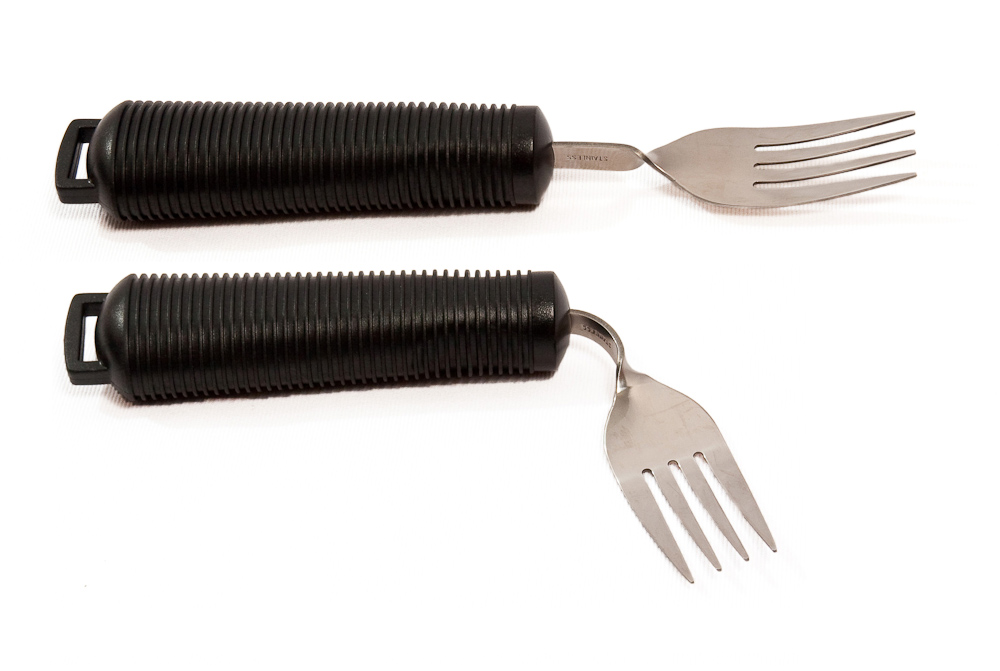
\includegraphics[width=5cm]{../figuras/talher.jpg}\\
			Fonte:\cite{vivere}
    
    \label{fig:talher}
  \end{center}
\end{figure}

A Figura \ref{fig:talher} mostra dois talheres que possuem cabos maiores para facilitar o manuseio, e um deles � ``dobrado'' para facilitar o posicionamento dos mesmos. Pacientes com quadros apresentados de Hemiplegia, Diplegia e algumas formas mistas podem se beneficiar com este tipo de talher.

}
\item{\acf{CAA}. Recursos eletr�nicos ou n�o para pessoas sem fala ou com limita��es dela (e.g., pranchas de comunica��o, vocalizadores, e softwares). A Figura \ref{fig:prancha} � um exemplo de prancha de comunica��o.

\begin{figure}[bth!]
  \begin{center}
    \caption{Exemplo de prancha de comunica��o}\vspace{.2cm}
			
      \centering
      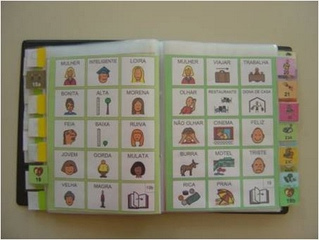
\includegraphics[width=5cm]{../figuras/prancha.jpg}\\
			Fonte:\cite{assistiva}
    
    \label{fig:prancha}
  \end{center}
\end{figure}

As pranchas de comunica��o exemplificadas na Figura \ref{fig:prancha} s�o meios de comunica��o para as pessoas com fala comprometida, isso pode ocorrer em todos os casos cl�nicos da \ac{PC}.

}
\item{Acessibilidade ao computador (e.g., teclados modificados, leitor de tela e ampliador de tela). A Figura \ref{fig:teclado} � um exemplo de teclado em modificado.
\vspace{-.5cm}
\begin{figure}[bth!]
  \begin{center}
    \caption{Exemplo de teclado em braile }\vspace{.2cm}
			
      \centering
      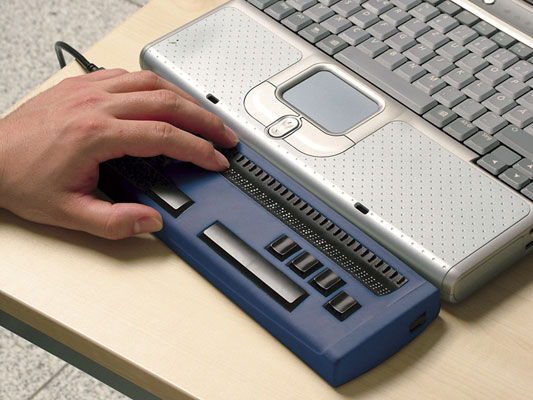
\includegraphics[width=4cm]{../figuras/teclado.jpg}\\
			Fonte:\cite{teclado}
    
    \label{fig:teclado}
  \end{center}
\end{figure}

A Figura \ref{fig:teclado} mostra que nos teclados modificados, a impress�o do que referencia cada tecla � na verdade um s�mbolo usado no alfabeto braile.

}
\item{Sistemas de controle de ambientes, que permitem que pessoas com dificuldades motoras controlem equipamentos a dist�ncia. A Figura \ref{fig:controle} � um exemplo de controle remoto para cegos.
\vspace{-.5cm}

\begin{figure}[bth!]
  \begin{center}
    \caption{Exemplo de controle assistivo}\vspace{.2cm}
			
      \centering
      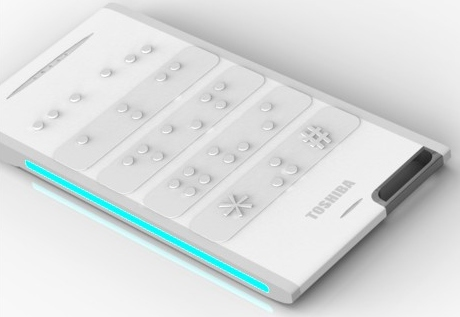
\includegraphics[width=4cm]{../figuras/controle.jpg}\\
			Fonte:\cite{controle}
    
    \label{fig:controle}
  \end{center}
\end{figure}
}
\vspace{-.5cm}
A Figura \ref{fig:controle} � um controle remoto que ao inv�s de possuir teclas com desenhos das fun��es e n�meros, os bot�es s�o representados em braile, para que os cegos possam manipular objetos a dist�ncia.

\item{Projetos Arquitet�nicos (e.g., cal�adas com guia para cegos e rampas de acesso). A Figura \ref{fig:rampa} � um exemplo de ramapa de acesso.

\begin{figure}[bth!]
  \begin{center}
    \caption{Exemplo de rampa de acesso}\vspace{.2cm}
			
      \centering
      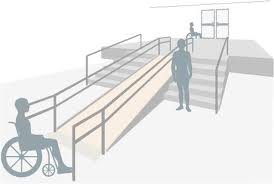
\includegraphics[width=4cm]{../figuras/rampa.jpg}\\
			Fonte:\cite{portal}
    
    \label{fig:rampa}
  \end{center}
\end{figure}

A Figura \ref{fig:rampa} representa uma rampa de acesso a cadeirantes, que torna poss�vel ao cadeirante o acesso a lugares mais elevados sem utilizar a ajuda de outras pessoas.

}
\item{�rteses e pr�teses, que permitem a troca ou ajuste de um membro. A Figura \ref{fig:protese} � um exemplo de pr�tese.
\vspace{-.5cm}
\begin{figure}[bth!]
  \begin{center}
    \caption{Exemplo de pr�tese}\vspace{.2cm}
			
      \centering
      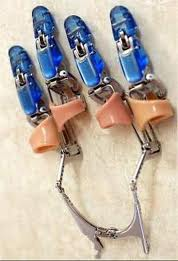
\includegraphics[width=3cm]{../figuras/protese.jpg}\\
			Fonte:\cite{protese}
    
    \label{fig:protese}
  \end{center}
\end{figure}
\vspace{-.5cm}
As pr�teses exemplificadas na Figura \ref{fig:protese}, ajudam as pessoas com membros danificados ou perdidos, a reabilita��o de movimentos.

}
\item{Equipamentos de aux�lio a postura (e.g., almofadas anat�micas e cintos). A Figura \ref{fig:cadeira} � um exemplo de cadeira de rodas com ajuste de postura.
\vspace{.5cm}
\begin{figure}[bth!]
  \begin{center}
    \caption{Exemplo de cadeira com regulagem de postura}\vspace{.2cm}
			
      \centering
      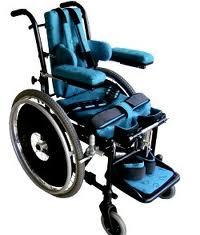
\includegraphics[width=4cm]{../figuras/cadeira.jpg}\\
			Fonte \cite{cadeira}
    
    \label{fig:cadeira}
  \end{center}
\end{figure}
}

Na Figura \ref{fig:cadeira} � poss�vel perceber o cinto na cadeira de rodas, que regulam a postura da pessoas do usu�rio.

\item{Equipamentos de mobilidade (e.g., cadeira de rodas motorizadas ou n�o e andadores). A Figura \ref{fig:cadeiramotorizada} representa um exemplo de cadeira de rodas motorizada.
\vspace{2cm}
\begin{figure}[bth!]
  \begin{center}
    \caption{Exemplo de cadeira de rodas motorizadas}
			
      \centering
      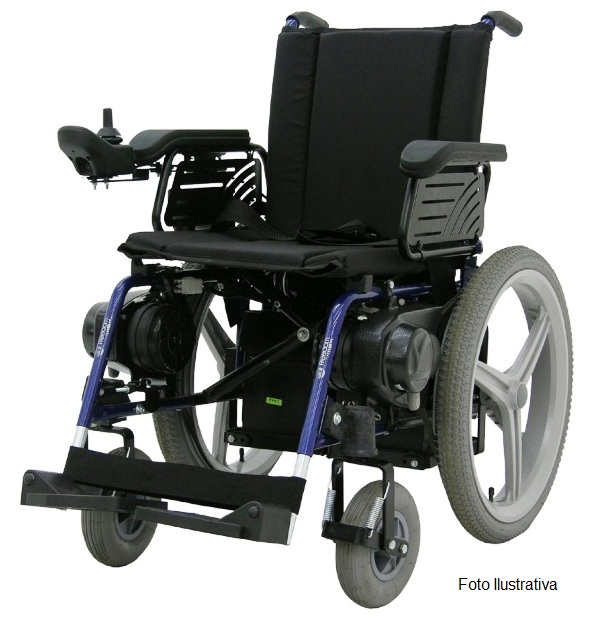
\includegraphics[width=3.5cm]{../figuras/cadeiramotorizada.jpg}\\
			Fonte: \cite{cinta}
    
    \label{fig:cadeiramotorizada}
  \end{center}
\end{figure}

Na Figura \ref{fig:cadeiramotorizada}, a cadeira possui um motor el�trico que faz com que a pessoa que a utiliza n�o necessite de grande esfor�o f�sico para moviment�-la.


}
\item{Aux�lio de surdos ou com audi��o parcial (e.g., aparelhos de surdez e telefones com teclado). A Figura \ref{fig:aparelhosurdez} � um exemplo de aparelho de surdez.
\vspace{-.5cm}
\begin{figure}[bth!]
  \begin{center}
    \caption{Exemplo de aparelho de surdez}
			
      \centering
      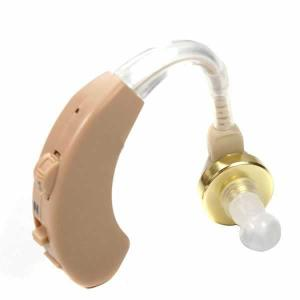
\includegraphics[width=3.5cm]{../figuras/aparelhosurdez.jpg}\\
			Fonte: \cite{surdez}
    
    \label{fig:aparelhosurdez}
  \end{center}
\end{figure}
}
\vspace{-.5cm}

Os aparelhos de surdez ilustrados pela Figura \ref{fig:aparelhosurdez} possibilitam que o �udio seja amplificado para que pessoas com defici�ncia auditiva parcial, possam escutar normalmente.

\item{Adapta��es a ve�culos. A Figura \ref{fig:carro} � um exemplo de carro adaptado a pessoas com defici�ncias f�sicas.
\begin{figure}[bth!]
  \begin{center}
    \caption{Exemplo de carro adaptado}\vspace{.2cm}
			
      \centering
      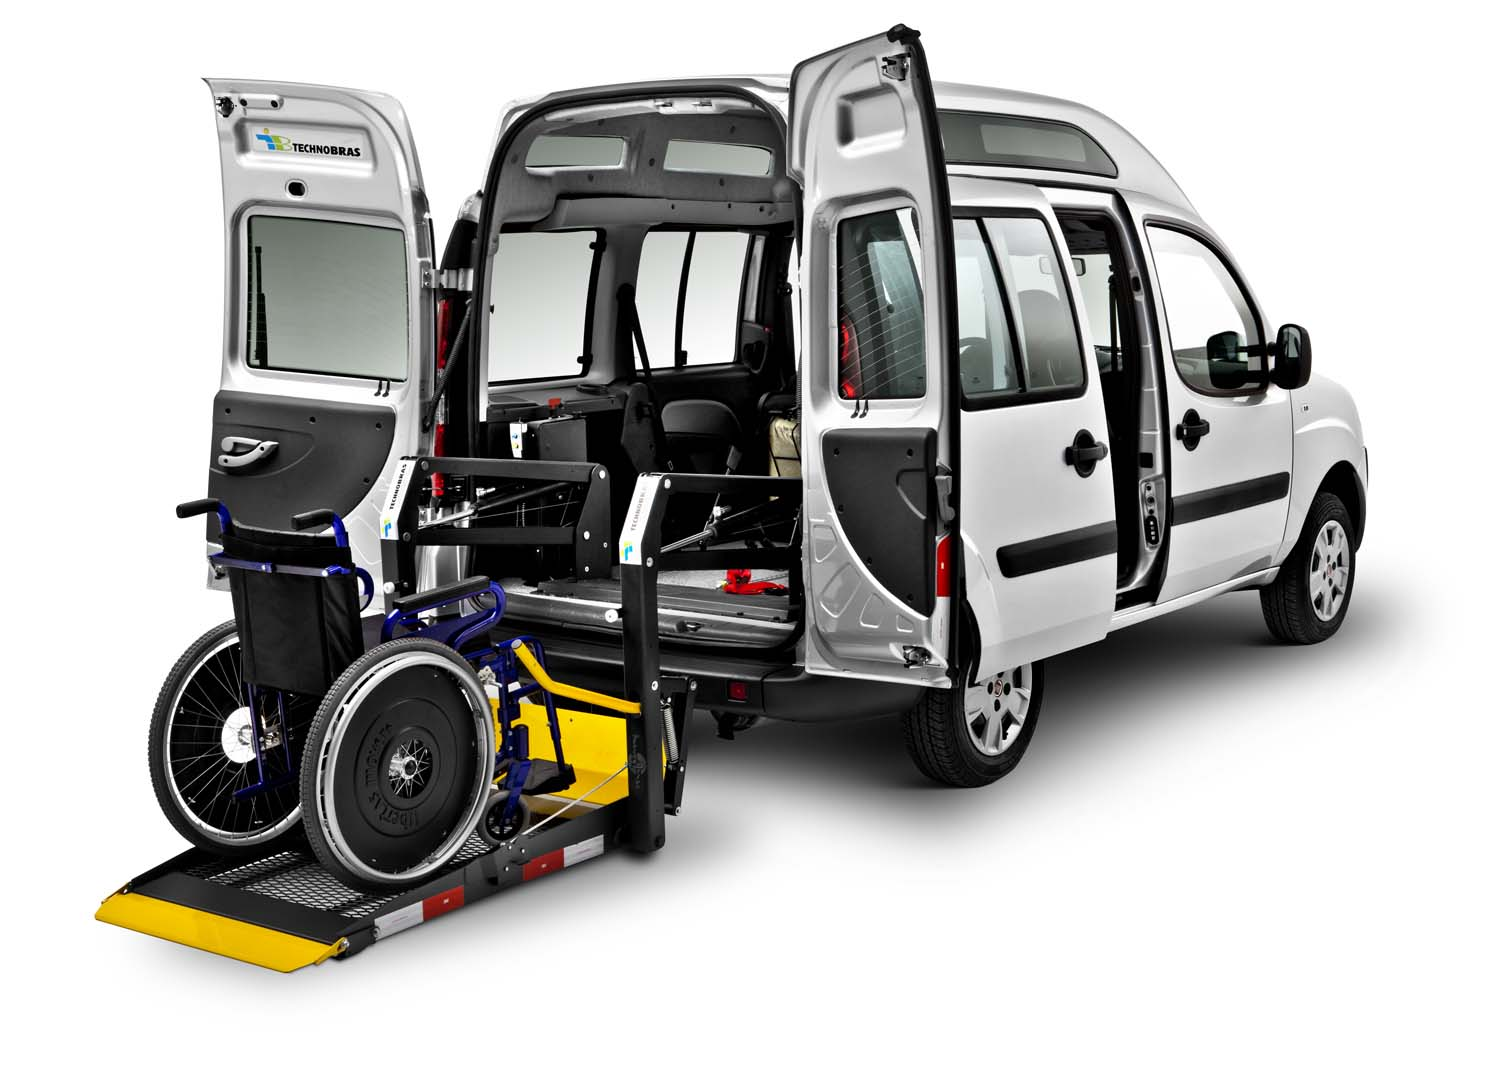
\includegraphics[width=4cm]{../figuras/carro.jpg}\\
			Fonte: \cite{fiat}
    
    \label{fig:carro}
  \end{center}
\end{figure}
}

A Figura \ref{fig:carro} � um exemplo de carro adaptado para pessoas com defici�ncia f�sica, possibilita que estas pessoas possam utilizar um ve�culo autonomamente.


\end{enumerate}


J� segundo a norma ISO 9999:2011(Anexo~\ref{iso9999}), a classifica��o das \ac{TA} se divide em categorias semelhante as diretrizes da \ac{ADA} por�m s�o mais espec�ficas. Para fins te�ricos, � utilizado no trabalho a classifica��o com base nas diretrizes da \ac{ADA} porque al�m da ISO 9999:2011 n�o incluir produtos e equipamentos usados exclusivamente por profissionais de sa�de e dispositivos implantados, a classifica��o \ac{ADA} apresenta um grupo de servi�os de \ac{TA} que promove o apoio � avalia��o da pessoa com defici�ncia, o desenvolvimento e personaliza��o de recursos, a integra��o da \ac{TA} com a��o e objetivos educacionais e de reabilita��o, e os apoios legais de concess�o \cite{corde}.


Uma pesquisa do \ac{W3C} \cite{wc} brasileiro aponta que das pessoas que usam aparelhos de \ac{TA}, 85\% � o computador o dispositivo mais usado, seguido do celular, {\it smarthphone} com 9\%, {\it tablet} com 2\%, e outros dispositivos com 4\%. Sendo cada vez mais necess�rio que existam op��es para esse tipo de p�blico dentro do acesso a informa��o.

A \ac{TA} faz parte da tecnologia, � a parte que auxilia a integra��o das pessoas que possuem algum tipo de defici�ncia. � uma �rea que envolve grandes por��es da popula��o, e que necessita de um cuidado especial, pois envolve al�m da pessoa com defici�ncia, as pessoas nos ambientes em que ela est� inserida.

\subsection{Legisla��o espec�fica de \acf{TA}}

Em rela��o a legisla��o de \ac{TA} alguns decretos s�o relevantes, entre eles a promulga��o do Decreto 3.298 
de 1999, que no artigo 19, fala do direito do cidad�o brasileiro com defici�ncia �s \ac{TA}. 
Nele consta que\cite{lima} (ver anexo {\ref{decreto1}}): 
\begin{quotation}
``Consideram-se ajudas t�cnicas, para os efeitos deste Decreto, os elementos que permitem 
compensar uma ou mais limita��es funcionais motoras, sensoriais ou mentais da pessoa 
portadora de defici�ncia, com o objetivo de permitir-lhe superar as barreiras da comunica��o e da 
mobilidade e de possibilitar sua plena inclus�o social. 
Par�grafo �nico. S�o ajudas t�cnicas:[...]elementos especiais para facilitar a comunica��o, a informa��o e a sinaliza��o para 
pessoa portadora de defici�ncia[...]``
\end{quotation}

O artigo 19 generaliza o termo Ajudas T�cnicas a todos os elementos que compensam limita��es do ser humano, por�m sem caracteriza��o ou classifica��o objetiva de tais ajudas. Tamb�m relevante, o decreto 5.296 de 2002, que d� prioridade de atendimento e estabelece normas gerais e crit�rios b�sicos para a promo��o da acessibilidade das pessoas com defici�ncia ou com 
mobilidade reduzida, possui um cap�tulo espec�fico sobre as ajudas t�cnicas no qual descreve 
v�rias inten��es governamentais na �rea da \ac{TA}, al�m de referir a constitui��o do 
\ac{CAT}. Neste decreto encontra-se que\cite{lima}: 
\begin{quotation}
``Consideram-se ajudas t�cnicas os produtos, instrumentos, equipamentos ou tecnologia 
adaptados ou especialmente projetados para melhorar a funcionalidade de pessoas portadoras de  
defici�ncia, com habilidade reduzida favorecendo autonomia pessoal, total ou assistida" .
\end{quotation}

No decreto 5.296\cite{cata} a legisla��o cita ao inv�s da compensa��o como no artigo 19, a autonomia total ou assistida das pessoas com defici�ncia. Embora esse Comit� leve a express�o ``Ajudas T�cnicas'' em sua 
denomina��o, tamb�m porque � a express�o prevista na legisla��o brasileira, 
os estudos desenvolvidos apontam e sugerem que as express�es 
``Tecnologia Assistiva'', ``Ajudas T�cnicas'' e ``Tecnologia de Apoio'', neste 
momento, continuem sendo entendidas como sin�nimos e que correspondam 
�s bases conceituais aprovadas pelo Comit�. Entretanto, estabelece a 
utiliza��o �nica da express�o ``Tecnologia Assistiva'' em seus documentos, 
como a mais apropriada, pelos seguintes motivos \apud{cata}{galvao}: 
\begin{itemize}
 
\item Por ser uma tend�ncia nacional j� firmada no meio acad�mico, nas 
organiza��es de pessoas com defici�ncia, em setores governamentais 
(Minist�rio MEC da Educa��o, Minist�rio da Ci�ncia e Tecnologia (MCT), Conselho Nacional de Desenvolvimento Cient�fico e Tecnol�gico CNPq), Institutos de Pesquisa (ITS Brasil) e no mercado de produtos; 
 
\item Pelo primeiro objetivo do Comit� de Ajudas T�cnicas, expl�cito no Artigo 
66 do Decreto 5296/2004, relativo � estrutura��o das diretrizes da �rea 
do conhecimento. A express�o Tecnologia Assistiva seria a mais 
compat�vel como a denomina��o de uma �rea de conhecimento, a ser 
oficialmente reconhecida; e
 
\item Por ser uma express�o bastante espec�fica ao conceito ao qual 
representa, diferentemente das express�es ``Ajudas T�cnicas'' e 
``Tecnologia de Apoio'', que s�o mais gen�ricas e tamb�m utilizadas para 
referirem-se a outros conceitos e realidades diferentes. 
\end{itemize}

Conforme votado e aprovado por unanimidade na quinta Reuni�o desse Comit�, al�m da determina��o de utiliza��o �nica da express�o Tecnologia Assistiva, foi decidido tamb�m que essa express�o seja utilizada no singular, por referir-se a uma �rea do conhecimento e sugere-se que se fa�am os poss�veis encaminhamentos para a revis�o da nomenclatura em 
instrumentos legais no pa�s. Este mesmo Comit� de Ajudas T�cnicas tamb�m aprovou, na sua terceira Reuni�o de abril de 2007, as bases conceituais que situam a Tecnologia Assistiva nos seguintes marcos \cite{cata,catb}: 

\begin{itemize}
\item �rea do Conhecimento;
\item Multidisciplinariedade;
\item Objetivos: promover a funcionalidade (atividade, participa��o) de 
pessoas com defici�ncia, mobilidade reduzida, ou idosas, visando sua 
autonomia, independ�ncia, qualidade de vida e inclus�o social; 
\item Composi��o: produtos, recursos, estrat�gias, pr�ticas, processos, 
m�todos e servi�os; e 
\item Ter presente os princ�pios do {\it Universal Design}\footnote{O conceito de Desenho Universal, ou ``{\it Universal Design}'', ou tamb�m chamado ``Desenho para todos'', � estudado a partir de alguns princ�pios tais como: equipara��o nas possibilidades de uso; flexibilidade no uso; uso simples e intuitivo; capta��o da informa��o; toler�ncia ao erro: m�nimo esfor�o f�sico; dimens�o e espa�o para uso e intera��o \cite{sepro}} e ITS BRASIL (Instituto de Tecnologia Social).

\end{itemize}

Apesar de uma iniciativa e uma legisla��o recente os assuntos acessibilidade e ajudas t�cnicas vem entrando no cotidiano dos brasileiros, pois h� uma cobran�a da parte governamental. Por�m, ainda existe uma defici�ncia em normas e na pr�pria legisla��o que regulamente as \ac{TA} principalmente na parte de classifica��o e exig�ncias.

\subsection{Iniciativas de \ac{TA}}
\label{iniciativas}

Existem v�rias iniciativas de \ac{TA} pelo mundo, como a  Funda��o SIDAR\cite{sidar} ({\it Seminario Iberoamericano sobre Diversidad y Accesibilidad en la Red}) que � uma institui��o de observa��o e recomenda��o na �rea da acessibilidade e inclus�o digital para os territ�rios ibero-americanos, a ATI\cite{ati} ({\it Assistive Technology Initiative}) na Universidade De George Mason na Virg�nia nos Estado Unidos, o INCNESI\cite{incnesi} (Iniciativa Nacional para os Cidad�os com Necessidades Especiais na Sociedade da Informa��o) que incentiva o uso de equipamentos para pessoas com defici�ncia em Portugal. 

Ainda no �mbito europeu, em 1999 foi organizado o Cons�rio \ac{EUSTAT} que desenvolveu um estudo entre 1997 e 1999, no contexto do Programa de Aplica��es Telem�ticas da Comiss�o Europeia, destinado a forma��o de usu�rios finais de \ac{TA}, envolvendo pessoas com defici�ncia ou idosos, seus familiares e profissionais assistentes pessoais, para que os mesmos pudessem fazer escolhas informadas, adequadas e respons�veis em rela��o a essas tecnologias. Esse estudo parte do princ�pio de que � fundamental a participa��o de usu�rio final como parceiro ativo na escolha das \ac{TA} que utiliza\cite{galvao}.

S�o parceiros do Cons�rcio \ac{EUSTAT} as seguintes organiza��es \cite{eustat}:

\begin{itemize}

\item SIVA {\it Servizio Informacione e Valutazione Ausili da Fondazione Dom Carlo Ghocchi Onlus}, da It�lia. Possui um centro de Inova��o e Transfer�ncia de Tecnologia, que incentiva projetos para autonomia de pessoas com defici�ncias;

\item CAPS  Centro de An�lise e Processamento de Sinais, do Instituto Superior T�cnico de Lisboa, Portugal;

\item \it{Association Nationale pour le Logement des personnes handicap�es}, da B�lgica;

\item \it{Groupement pour l�insertion des personnes handicap�es physiques}, da Fran�a;

\item \it{Danish Centre for Technical Aids for Rehabilitation and Education}, da Dinamarca; e

\item \it{Centro Studi Prisma}, da It�lia.

\end{itemize}

Os estudos que s�o parceiros do cons�rcio, s�o centros de refer�ncia em \ac{TA} na Europa, juntas s�o respons�veis por uma parte consider�vel de publica��es, dispositivos, sobre \ac{TA}. O Cons�rcio EUSTAT recomenda a classifica��o \ac{HEART} que prop�e tr�s grandes �reas de forma��o em 
rela��o �s \ac{TA}:
\begin{itemize} 
\item Componentes t�cnicos;
\item Componentes humanos; e
\item Componentes socioecon�micos.
\end{itemize}

Essa classifica��o tem ganhado for�a na atualidade, principalmente em decorr�ncia do paradigma inclusivo, o qual desloca as limita��es de funcionalidade e possibilidades de participa��o do �mbito restrito � defici�ncia em si, para situ�-las a partir das barreiras impostas pelo ambiente f�sico e social\cite{rodrigues}. Como n�o foi encontrado uma padroniza��o mundial para a defini��o de \ac{TA} as diferentes iniciativas encontradas se relacionam na tabela \ref{tabeladois}.

\begin{table}[bth!]
\centering
\scriptsize
\caption{Tabela com as diferen�as de Iniciativas de \ac{TA} encontradas.}\vspace{.2cm}
 \begin{tabular}{|p{2cm} |  p{3.9cm} | p{3cm} | p{4cm}| }
    \hline
    Pa�s & Termo Utilizado (Tradu��o) & Classifica��o & Defini��o \\ \hline
    Brasil & Tecnologia Assistiva, Ajudas T�cnicas &Ca\-te\-go\-ri\-as relativas aos e\-qui\-pa\-men\-tos & Melhorar as pessoas com defici�ncia e mobilidade re\-du\-zi\-da \\ \hline
    EUTSTAT & Ajudas T�cnicas e Tecnologia de Apoio & Classifica��o por componentes& Compensar as pessoas com defici�ncia e idosas \\ \hline
    ADA & {\it Assistive Technology} (Tecnologia Assistiva) & Trata as situa��es & Ajudas aos indiv�duos com defici�ncia em situa��es es\-pe\-c�\-fi\-cas \\ \hline	
		\end{tabular}
    \label{tabeladois}
		\\Fonte: o pr�prio autor.

\end{table}

A tabela {\ref{tabeladois}} mostra as diferen�as das tr�s iniciativas mais relevantes encontradas. Apesar da mudan�a de termos, as iniciativas n�o possuem grandes diferen�as entre si. A classifica��o da \ac{TA} � o �nico fator que diferencia nas iniciativas. Por�m, a relev�ncia da mudan�a � pequena, em rela��o a as ajudas �s pessoas com defici�ncia.


\section{Comunica��o Alternativa Ampliada (CAA)}

Na \ac{TA}, como mencionado anteriormente na se��o {\ref{Tecnologia Assistiva}} se divide em algumas classifica��es, dentro delas temos a \ac{CAA}, que � linha de pesquisa adotada neste trabalho. A \ac{CAA} abrange qualquer meio de comunica��o que suplemente ou substitua os m�todos naturais de fala ou escrita. � um meio que auxilia a comunica��o de um indiv�duo com outras pessoas. Os sistemas de \ac{CAA} podem ser divididos em pictoriais\footnote{Os sistemas pictoriais representam os referentes por analogia f�sica e n�o por conven��o arbitr�ria, o que lhes confere iconicidade e clareza denotativa, sendo bem compreendidos, aprendidos e lembrados por crian�as, estrangeiros e c�rebro-lesados. Contudo, o universo de significados que podem representar restringe-se ao imagin�vel \cite{fernando}.} e simb�licos\footnote{Os sistemas simb�licos representam referentes por conven��es arbitr�rias, usando regras de recombina��o e sintaxe espec�fica, o que resulta em opacidade denotativa, mas lhes permite representar virtualmente qualquer conceito, imagin�vel ou n�o \cite{fernando}.} podendo ser de alta tecnologia (e.g., sistemas computadorizados, e softwares especiais) e baixa tecnologia (e.g., simples, e n�o el�tricos) \cite{leydi}.

A \ac{CAA} � definida como uma maneira alternativa � comunica��o oral e escrita que compreende o uso de gestos, sinais manuais, express�es faciais, pranchas com s�mbolos pictogr�ficos, pranchas de alfabeto, comunicadores de voz gravada ou sintetizada at� sistemas sofisticados de computador \apud{glennen}{correia}. Inicialmente eram utilizados sistemas sem tecnologia, recorrendo apenas ao corpo humano, como a linguagem por sinais (e.g., libras) passando pelos sistemas anal�gicos ou de baixa tecnologia (e.g., cart�es e livros com s�mbolos e imagens) at� sistemas baseados em recursos computacionais (e.g., vocalizadores, e softwares para computador com s�ntese de voz) \apud{worthy}{correia}.

O trabalho da \ac{CAA} engloba uma s�rie de s�mbolos, recursos, estrat�gias e t�cnicas para auxiliar o desenvolvimento de uma comunica��o complementar. Os s�mbolos s�o as representa��es visuais, auditivas ou t�teis de um conceito; os recursos s�o os objetos ou equipamentos utilizados para transmitir as mensagens que podem ser pranchas de comunica��o, os comunicadores ou o computador; as t�cnicas s�o as formas como as mensagens s�o transmitidas e as estrat�gias referem-se ao modo como os recursos da \ac{CA} s�o utilizados \apud{king}{pelosi2}.

Como o foco deste trabalho � encontrar uma solu��o alternativa a pessoas que possuem defici�ncia na fala, em conjunto com defici�ncia motora (quadros tabela cl�nicos), a \ac{CAA} � a abordagem encontrada que melhor se encaixa neste contexto. Pois a \ac{CAA} utiliza estrat�gias e t�cnicas para o desenvolvimento de uma comunica��o complementar, que auxiliam a suplementa��o ou substitui��o da forma natural de comunica��o.


\section{Considera��es do Cap�tulo}

Com a pesquisa realizada no cap�tulo {\ref{cap:introducao}}, fica evidenciado que pessoas com necessidades especiais, precisam de recursos que supram ou compensem suas defici�ncias para que possam ser inseridas na sociedade. Apesar de uma por��o consider�vel da popula��o mundial possuir algum tipo de defici�ncia, os estudos e legisla��o sobre a \ac{TA} s�o consideravelmente recentes.
	
Al�m disso, vale ressaltar a import�ncia de que se desenvolva mais solu��es de \ac{TA}, principalmente acess�veis, e que os desenvolvedores, se preocupem com o ambiente em que esta pessoa est� inserida e as pessoas com as quais ela ir� interagir. Foram necess�rios conhecimentos sobre \ac{TA}, \ac{CAA} e acessibilidade para que se entenda o foco deste trabalho que visa encontrar uma solu��o alternativa de \ac{CAA} para pessoas que possuem \ac{PC} que apresentam defici�ncia motora e de fala.
	
Este trabalho se enquadra na Lei no 10.098, de dezembro de 2000 que estabelece crit�rios como o artigo 17 que garante direito de comunica��o e express�o por mecanismos, ou alternativas t�cnicas. Al�m disso, se enquadra tamb�m, no Decreto 5296/2004, Artigo 66 do Comit� de Ajudas T�cnicas, no qual estabelece o termo \acf{TA} como a denomina��o mais compat�vel ao tema.

O trabalho tamb�m pode ser classificado nas diretrizes da \ac{ADA} como um trabalho no contexto de \acf{CAA}. J� na norma ISO 9999:2011 na subcategoria, Produtos de Apoio para Treino de Comunica��o Alternativa e Aumentativa, c�digo 05 06 27, categoria Produtos de apoio para treino de comunica��o com imagens e desenhos.
     %chamada de arquivo introducao.tex
\chapter{Defini��o do Problema}


Ap�s a an�lise das pesquisas realizadas no cap�tulo \ref{cap:introducao}, nota-se que o estudo de \ac{TA} � recente, e que ainda n�o h� meios suficientes para possibilitar a inclus�o de uma parte consider�vel de pessoas com defici�ncia. A \ac{CAA} pode ser utilizada junto � popula��o de paralisados cerebrais, pessoas com defici�ncia mental e autistas \cite{darcy}. Contudo, a Comunica��o Alternativa no contexto espec�fico do trabalho, pretende apenas atender o problema que as pessoas com \ac{PC} nos quadros cl�nicos 1, 3, 4 ,5 e 6, tem ao se comunicar com seus terapeutas. Uma das solu��es encontradas pelos terapeutas � a prancha de comunica��o mencionada na se��o \ref{classificacao} e que utiliza a comunica��o atrav�s de imagens e texto.

\section{Prancha de Comunica��o}

A prancha de comunica��o � formada por um conjunto de s�mbolos, no qual o paciente aponta o s�mbolo que representa o que ele deseja expressar. Os s�mbolos s�o as formas de representa��o de objetos, pessoas, a��es, rela��es e conceitos \cite{darcy,bersch}. 

\begin{figure}[bth!]
  \begin{center}
    \caption{Prancha de Comunica��o}\vspace{.2cm}
			
      \centering
      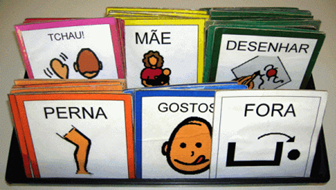
\includegraphics[width=5cm]{../figuras/prancha.png}\\
			Fonte: \cite{assistiva}.
    \vspace{-1cm}
    \label{pranchaa}
  \end{center}
\end{figure}

As pranchas devem ser personalizadas de acordo com as possibilidades de a��o da pessoa com defici�ncia, ou seja, o terapeuta � respons�vel por avaliar cada caso e escolher as categorias de s�mbolos, e outras configura��es (e.g., tamanho dos s�mbolos, complexidade de frases e quantidade de s�mbolos). Os crit�rios para escolha das pessoas que utilizaram a solu��o n�o s�o abordados neste trabalho, pois n�o fazem parte do escopo.

No sentido de compreender os requisitos do usu�rio, que � espec�fico\cite{bersch} foi elaborado um question�rio, que foi respondido na entrevista concedida pela psic�loga respons�vel pelo atendimento psicol�gico focalizado na reabilita��o e inclus�o social, escolar e no trabalho, de pessoas com defici�ncia f�sica na \ac{ARCD} \cite{juliane}. Analisando o question�rio (Ap�ndice \ref{apendice2}) podem ser mencionados como problemas da solu��o prancha de comunica��o:

\begin{itemize}
\item Como a prancha pode conter muitos s�mbolos, as pessoas t�m dificuldade em manuse�-la;
\item A altera��o dos s�mbolos depende de novas impress�es de p�ginas, que geram novos custos, deslocamentos e tempo na agenda do terapeuta;
\item Os softwares para desenvolvimento de pranchas tem um custo elevado;
\item Limita��o a percep��o e mem�ria visual;
\item Pacientes, familiares ou funcion�rios da escola tendem a perder as pranchas;
\item Como � feita de papel, a deteriora��o das p�ginas acontecem com o tempo; e
\item Tamanho dos s�mbolos, dependendo do grau de les�o da pessoa com \ac{PC}, ela tem maior dificuldade em apontar os s�mbolos quando estes s�o pequenos, ocasionando em p�ginas com poucos s�mbolos, maior n�mero de p�ginas a serem impressas, maior custo de impress�o a cada vez que a prancha for alterada, e a n�o reutiliza��o da prancha com outras pessoas.
\end{itemize}

N�o foi encontrado na literatura outros problemas em rela��o a solu��o prancha de comunica��o. A solu��o proposta consiste em emular a prancha de comunica��o em um software, que ofere�a as mesmas caracter�sticas que uma prancha de comunica��o tradicional em papel, por�m com as facilidades de estar em uma plataforma digital. Uma funcionalidade que � adicionada � a vocaliza��o da frase relacionada ao pictograma\footnote{Pictogramas s�o s�mbolos gr�ficos de utilidade p�blica; comunicam informa��es, instru��es, advert�ncias e prescri��es por meio de desenhos concisos e esquematizados \cite{pictograma}}, com o prop�sito de aumentar o processo cognitivo do usu�rio com mais um sentido a ser trabalhado.
\vspace{2cm}
\section{Identifica��o dos requisitos}
\label{req}

Para que a proposta atenda as necessidades e restri��es do problema, alguns requisitos\footnote{Requisitos de um sistema s�o descri��es dos servi�os que devem ser fornecidos por esse sistema e as suas restri��es operacionais. Os requisitos podem ser classificados como requisitos funcionais que s�o declara��es de servi�os que o sistema deve prover, descrevendo o que o sistema deve fazer, e os requisitos n�o-funcionais que descrevem restri��es sobre os servi�os ou fun��es oferecidos pelo sistema \cite{som2007}} funcionais e outros n�o funcionais foram levantados com o aux�lio do Grupo Assistiva\footnote{Assistiva Tecnologia para a Inclus�o Social, � um grupo que visa sanar problemas enfrentados por deficientes e dificuldades dos terapeutas ocupacionais que cuidam destes, nas associa��es de Joinville, SC. http://www.assistiva.joinville.udesc.br}. Atrav�s do grupo foram feitos contatos com parceiros, como a \ac{ACE}, a \ac{ADEJ} e a \ac{APAE}. Atrav�s desses contatos foram levantados alguns requisitos fundamentais para que a solu��o proposta abranja o escopo do problema.

\noindent
Requisitos Funcionais:

\begin{enumerate}
\item A solu��o proposta deve apresentar uma grade de pictogramas;
\item A solu��o deve aceitar diferentes formatos de s�mbolos e cores;
\item A solu��o deve aceitar s�mbolos criados pelo terapeuta;
\item Novos s�mbolos devem ser adicionados a grade de pictogramas sem que o usu�rio tenha experi�ncia no uso da solu��o;
\item A exclus�o de s�mbolos deve ser facilitada, ou seja, mesmo que a experi�ncia do usu�rio na solu��o seja pequena, ele deve conseguir realizar a tarefa;
\item A solu��o dever� vocalizar a frase pr�-estabelecida relacionada ao pictograma, quando este for selecionado;
\item O usu�rio mesmo com defici�ncia deve conseguir executar os pictogramas da solu��o; 
\item A solu��o deve representar o que o usu�rio est� querendo expressar da melhor maneira poss�vel (e.g., entona��o e pontua��o);
\item Todos os s�mbolos devem ser acessados de uma forma simples, ou seja, sem categorias e arquiteturas complexas; e
\item Os s�mbolos devem ter tamanhos edit�veis.
\end{enumerate}

\noindent
Requisitos N�o Funcionais:

\begin{enumerate}
\item A solu��o tem que ser permanente, ou seja, guardar os s�mbolos e sua sequ�ncia;
\item A solu��o deve estar dispon�vel e deve ser acess�vel a todas as pessoas, atrav�s do software disponibilizado em reposit�rios p�blicos;
\item O tempo de resposta da solu��o n�o deve causar frustra��o ao usu�rio, ou seja, a vocaliza��o da frase deve ser em um tempo menor a dois segundos;
\item A utiliza��o da solu��o n�o deve depender do uso da Internet;
\item A  licen�a da solu��o dever� permitir que outros pesquisadores possam aprimor�-la; 
\item A solu��o deve ser intuitiva sem necessitar de um longo aprendizado para manuse�-la; e
\item A solu��o deve estar em uma plataforma que aceite diferentes tipos de interface de entrada (e.g., mouse alternativo, aceler�metros e dispositivos espec�ficos de uma defici�ncia).
\end{enumerate}



Como abordado no cap�tulo \ref{cap:introducao}, a legisla��o n�o define crit�rios obrigat�rios para solu��es de \ac{CAA}. Contudo, o trabalho seguir� as recomenda��es mencionadas sobre \ac{TA} na se��o \ref{Tecnologia Assistiva}. Ap�s a an�lise de requisitos funcionais e n�o funcionais, uma alternativa encontrada � a informatiza��o da solu��o. Para o melhor compreendimento do escopo do trabalho, foi elaborada uma pesquisa sobre o problema e suas poss�veis solu��es e foram identificados trabalhos correlatos.

\vspace{4cm}


\section{Trabalhos Correlatos}

Durante a pesquisa foram encontrados trabalhos e iniciativas de \ac{TA} e a \ac{CAA}, citados na se��o \ref{iniciativas}, por�m apenas uma parte abrange o escopo do problema, os trabalhos correlatos identificados foram:

\begin{enumerate}

\item{Prancha Multiplataforma Livre\cite{puc} (prancha pictogr�fica virtual), projeto desenvolvido por alunos da Pont�fica Universidade Cat�lica do Paran�, projeto desenvolvido em 2010, de c�digo livre licen�a GPL\footnote{Licen�a GPL � uma licen�a que permite que os programas sejam distribu�dos e 
reaproveitados mantendo os direitos do autor.}, e utilizado em computadores pessoais;}

\item{Livox\cite{livox}, � um produto de licen�a propriet�ria, que pode ser utilizado em {\it tablets} com sistema Android, da empresa Agora Eu Consigo Tecnologias de Inclus�o Social Ltda, empresa do segmento de Neg�cios Sociais, voltada para o desenvolvimento de produtos, solu��es, servi�os e treinamentos que viabilizem a inclus�o social e a acessibilidade de pessoas com necessidades especiais ao conv�cio familiar e social; e}

\item{Que-Fala\cite{quefala}, � um produto de licen�a propriet�ria, que pode ser utilizado em sistemas Android e Computadores Pessoais, da empresa M�todos Solu��es Inteligentes cujo o objetivo principal � dar acessibilidade e possibilitar a inclus�o das pessoas com defici�ncia na sociedade, facilitando o cotidiano dessas pessoas atrav�s de solu��es tecnol�gicas.}

\end{enumerate}

Os trabalhos correlatos identificados s�o de tipos de institui��es diferentes (e.g., p�blicas e privadas), trabalham em plataformas diferentes (e.g., {\it smartphones} e computador pessoal) e utilizam abordagens diferentes em rela��o ao usu�rio e ao contexto no qual est� inserido. Por�m, todos foram feitos para problemas semelhantes ao escopo do trabalho.   
\vspace{3cm}
\subsection{Compara��o de trabalhos correlatos com requisitos}

Para o maior entendimento em rela��o aos requisitos da solu��o e ao trabalhos correlatos encontrados, a tabela \ref{tabela_correlatos} apresenta quais requisitos funcionais que os trabalhos correlatos contemplam, e a tabela \ref{tabela_correlatos2}, apresenta os requisitos n�o funcionais, que os trabalhos correlatos contemplam.

\begin{table}[bth!]
\centering
\scriptsize
\caption{Tabela da compara��o de requisitos funcionais com trabalhos correlatos}\vspace{.2cm}

	
    \begin{tabular}{ |p{6.5cm}|p{3cm}|p{1.5cm}|p{3cm}| }
		
    \hline
		
    Trabalho & Prancha Multiplataforma Livre & Livox & Que-Fala   \\ \hline \hline
		A solu��o proposta deve apresentar uma grade de pictogramas & OK  & OK  & OK \\ \hline 
		A solu��o deve aceitar diferentes formatos de s�mbolos e cores & OK & OK  & OK\\ \hline  
		A solu��o deve aceitar s�mbolos criados pelo terapeuta & N.A. (Apenas s�mbolos j� estabelecidos) & OK  & N.A. (Apenas s�mbolos j� estabelecidos)\\ \hline 
		Novos s�mbolos\- devem ser adicionados a grade \- sem que o usu�rio tenha \-experi�ncia no uso \-da solu��o & OK & N.A. & N.A. \\ \hline 
		 A exclus�o de s�mbolos deve ser facilitada, ou seja, mesmo que a experi�ncia do usu�rio na solu��o seja pequena, ele deve conseguir realizar a tarefa & OK  & N.A.  & N.A. \\ \hline 
		A solu��o deve representar o que o usu�rio est� querendo expressar da melhor maneira poss�vel (e.g., entona��o e pontua��o) & N.A. (Na vers�o dispon�vel a m�quina de vocaliza��o n�o funciona)  & OK  & OK  \\ \hline 
		O usu�rio mesmo com defici�ncia deve conseguir apertar nos s�mbolos da solu��o & OK & OK  & OK \\ \hline 
		Todos os s�mbolos devem ser acessados de uma forma simples, ou seja, sem categorias e arquiteturas complexas & OK  & OK  & N.A. \\ \hline 
		Os s�mbolos devem ter tamanhos edit�veis & N.A.  & OK  & N.A.\\ \hline 
		
    \end{tabular}
    \label{tabela_correlatos}
		
		Fonte: o pr�prio autor (N.A. N�o atendem).
		\vspace{-0.5cm}

\end{table}


Na tabela \ref{tabela_correlatos}, o software Livox n�o atende alguns requisitos funcionais por se tratar de uma solu��o em que necessita uma configura��o espec�fica por parte da empresa para cada usu�rio. Al�m disso um treinamento para o cuidador/cliente que adquire a licen�a do software � necess�rio. O software Que-Fala na vers�o em que foi identificada n�o atende boa parte dos requisitos funcionais identificados, principalmente em rela��o aos pictogramas. O software Prancha Multiplataforma Livre, apesar de ser um trabalho acad�mico, n�o foi encontrado quantidade expressiva de literatura a seu respeito e h� n�o conformidades em suas tarefas, como a n�o vocaliza��o das palavras ou travamento da solu��o.

\vspace{1cm}

\begin{table}[bth!]
\centering
\scriptsize
\caption{Tabela da compara��o de requisitos n�o funcionais com trabalhos correlatos}\vspace{.2cm}

	
    \begin{tabular}{ |p{6.5cm}|p{3cm}|p{3cm}|p{3cm}| }
		
    \hline
		
    Trabalho & Prancha Multiplataforma Livre & Livox & Que-Fala   \\ \hline \hline
		A solu��o tem que ser permanente, ou seja, guardar os s�mbolos e sua sequencia & OK & OK  & OK \\ \hline 
		A solu��o deve estar dispon�vel e deve ser acess�vel a todas as pessoas, atrav�s do software disponibilizado em reposit�rios p�blicos & OK (Licen�a GPL) & N.A.(Software Propriet�rio)  & N.A.(Software Propriet�rio)  \\ \hline  
		 O tempo de resposta da solu��o n�o deve causar frustra��o ao usu�rio, ou seja, a vocaliza��o da frase deve ser em um tempo menor a dois segundos & N.A.(Tempo de espera superior) & OK  & OK \\ \hline 
		A utiliza��o da solu��o n�o deve depender do uso da Internet & OK  & OK  & OK \\ \hline 
		 A licen�a da solu��o dever� permitir que outros pesquisadores possam aprimor�-la & OK (Possui licen�a GPL)  & N.A. (Licen�a propriet�ria) & N.A. (Licen�a Propriet�ria) \\ \hline 
		A solu��o deve estar em uma plataforma que aceite diferentes tipos de interface de entrada (e.g., mouse alternativo, aceler�metros e dispositivos espec�ficos de uma defici�ncia) &  OK &  N.A.(Sistema executa apenas em sistemas Android) & OK \\ \hline 
		
    \end{tabular}
    \label{tabela_correlatos2}
		\\Fonte: o pr�prio autor (N.A. N�o atendem).
		

\end{table}

As tabelas \ref{tabela_correlatos} e \ref{tabela_correlatos2} possibilitam comparar todos os requisitos com os trabalhos correlatos, e � poss�vel perceber que nem todos os requisitos s�o cumpridos por apenas um trabalho. Principalmente porque dois dos tr�s trabalhos encontrados, possuem licen�a propriet�ria, ou executam eu uma plataforma, que n�o aceite diferentes tipos de interface de entrada. Sendo assim, justifica-se a cria��o de uma proposta alternativa as que foram encontradas, e que atenda especificamente o problema definido e seus requisitos. 


\section{Conclus�es do Cap�tulo}

Como os trabalhos correlatos possuem contextos diferentes do contexto baseado na entrevista \cite{juliane}, fica evidente que uma nova alternativa � necess�ria para o est�mulo de pessoas com \ac{PC}. Principalmente as pessoas que n�o tem recursos financeiros o suficiente para a compra de uma solu��o propriet�ria, ou utilizam algum tipo alternativo de interface (e.g., mouse inclusivo) para entrada de dados nos sistemas. Fica evidenciado tamb�m, que os terapeutas necessitam de uma solu��o, com mais est�mulos ao usu�rio, que n�o gaste tanto tempo na prepara��o e que seja permanente.

\chapter{Proposta}
\label{cap:proposta}
\acresetall
Segundo a an�lise de requisitos do problema e dos trabalhos correlatos do cap�tulo \ref{cap:definicao_problema}, nota-se a necessidade de uma proposta que abranja tamb�m os requisitos n�o atendidos mencionados. Uma proposta que possibilite facilidade, do terapeuta e do usu�rio, que seja acess�vel, por�m sem perder suas funcionalidades principais. A ideia principal � desenvolver um software livre, de licen�a GPL que a interface seja intuitiva para a pessoa com \ac{PC}, e que leve em considera��o a experi�ncia de uso de softwares do terapeuta. A solu��o deve cumprir todos os requisitos funcionais e n�o funcionais identificados, e dever� ser desenvolvida considerando o ambiente de terapia ocupacional, no qual atuam a pessoa com defici�ncia e o terapeuta.

\section{Especifica��o da Proposta}
\label{esp}
A solu��o ser� desenvolvida em Java, para que atenda o requisito n�o funcional n�mero sete no qual fala que a solu��o  deve estar em uma plataforma que aceite diferentes tipos de entradas, pois Java pode ser executada em diferentes plataformas desde que comportem uma \ac{JVM}. Al�m disso, como Java segundo a Tiobe\cite{tiobe} � uma das linguagens mais populares do mundo, o c�digo poder� ser compreendido mais facilmente por outros programadores, podendo se utilizar da l�gica para ser migrado para outras plataformas (e.g., Android). 
Outro benef�cio da linguagem Java, � a f�cil adapta��o de \ac{APIS} e bibliotecas para a manipula��o de �udios e imagens que ser�o necess�rios para contemplar os requisitos funcionais de um, dois, tr�s e dez. Mesmo outras op��es de linguagens, que deixariam o programa com melhor desempenho e menor uso de mem�ria, como a linguagem C \cite{daniel}, a linguagem Java foi escolhida pela proximidade do desenvolvedor (autor) com a tecnologia.

A interface escolhida dentro da tecnologia Java, � a JFrame que j� implementa algumas funcionalidades (e.g., minimiza��o, maximiza��o, erros, bot�es, etc.). Neste interface ser� implementada uma grade de pictogramas para que atenda o requisito funcional n�mero um. Para que a proposta cumpra os requisitos funcionais quatro a seis e n�o funcionais tr�s e seis a solu��o ser� desenvolvida visando algumas metas de usabilidade como \cite{nielsen,iso2}:

\begin{itemize}
\item Facilidade de Aprendizado: a solu��o deve ser f�cil de assimilar pelo usu�rio, para que este possa come�ar a trabalhar rapidamente. 
\item Efici�ncia: a solu��o deve ser eficiente para que o usu�rio, depois de a saber usar, possa atingir uma boa produtividade;

\item Facilidade de Memoriza��o: a solu��o deve ser facilmente memorizada, para que depois de algum tempo sem a utilizar, o usu�rio se recorde como us�-la;
\item Erros: mensagens de erro claras, preven��o. Eliminar as condi��es pass�veis de erros ou verific�-las, apresentado aos usu�rios uma op��o de confirma��o antes de se comprometerem com uma determinada a��o; e

\item Satisfa��o: conforto e aceitabilidade da solu��o. 
\end{itemize}

Para que a vocaliza��o expresse o texto atribu�do aos pictogramas de melhor maneira poss�vel, foram pesquisadas algumas m�quinas de vocaliza��o de texto,(e.g., IVONA Speech Cloud \cite{ivona} e AT\&T Natural Voices� Text-to-Speech\cite{att}). Por�m, a �nica encontrada que atende os requisitos da solu��o, � a m�quina {\it Text-to-Speech} do Google. As outras m�quinas supracitadas s�o de licen�as propriet�rias, que impossibilitam a solu��o de cumprir o requisito n�o funcional n�mero dois ou n�o est�o dispon�veis na l�ngua portuguesa, que descumpririam o requisito n�o funcional n�mero oito. Como a m�quina do Google s� funciona se o dispositivo que a estiver executando estiver conectado a Internet, a solu��o salvar� o �udio dos pictogramas quando adicionados, permitindo que a solu��o possa ser utilizada quando o dispositivo estiver sem conex�o com a Internet. 

Com o intuito da solu��o cumprir o requisito funcional n�mero sete, a apresenta��o dos pictogramas na grade est�o dispostos em �rvore. Disposi��o utilizada na solu��o prancha de comunica��o \cite{darcy}. Sendo assim, ap�s a execu��o de um pictograma, a solu��o apresenta novos pictogramas relacionados ao anterior. Para a maior compreens�o a figura \ref{arvore} representa um exemplo de pictogramas retirados do \ac{ARASSAC}\cite{arassac}, que � o vencedor do pr�mio de acessibilidade universal de 2010, e oferece pictogramas sobre a licen�a {\it Creative Commons} CC BY-NC-SA\footnote{Esta licen�a permite que outros remixem, adaptem e criem a partir do seu trabalho para fins n�o comerciais, desde que atribuam a voc� o devido cr�dito e que licenciem as novas cria��es sob termos id�nticos.}. 

\begin{figure}[bth!]
  \begin{center}
    \caption{Figura que representa exemplo da disposi��o de pictogramas}\vspace{.2cm}
			
      \centering
      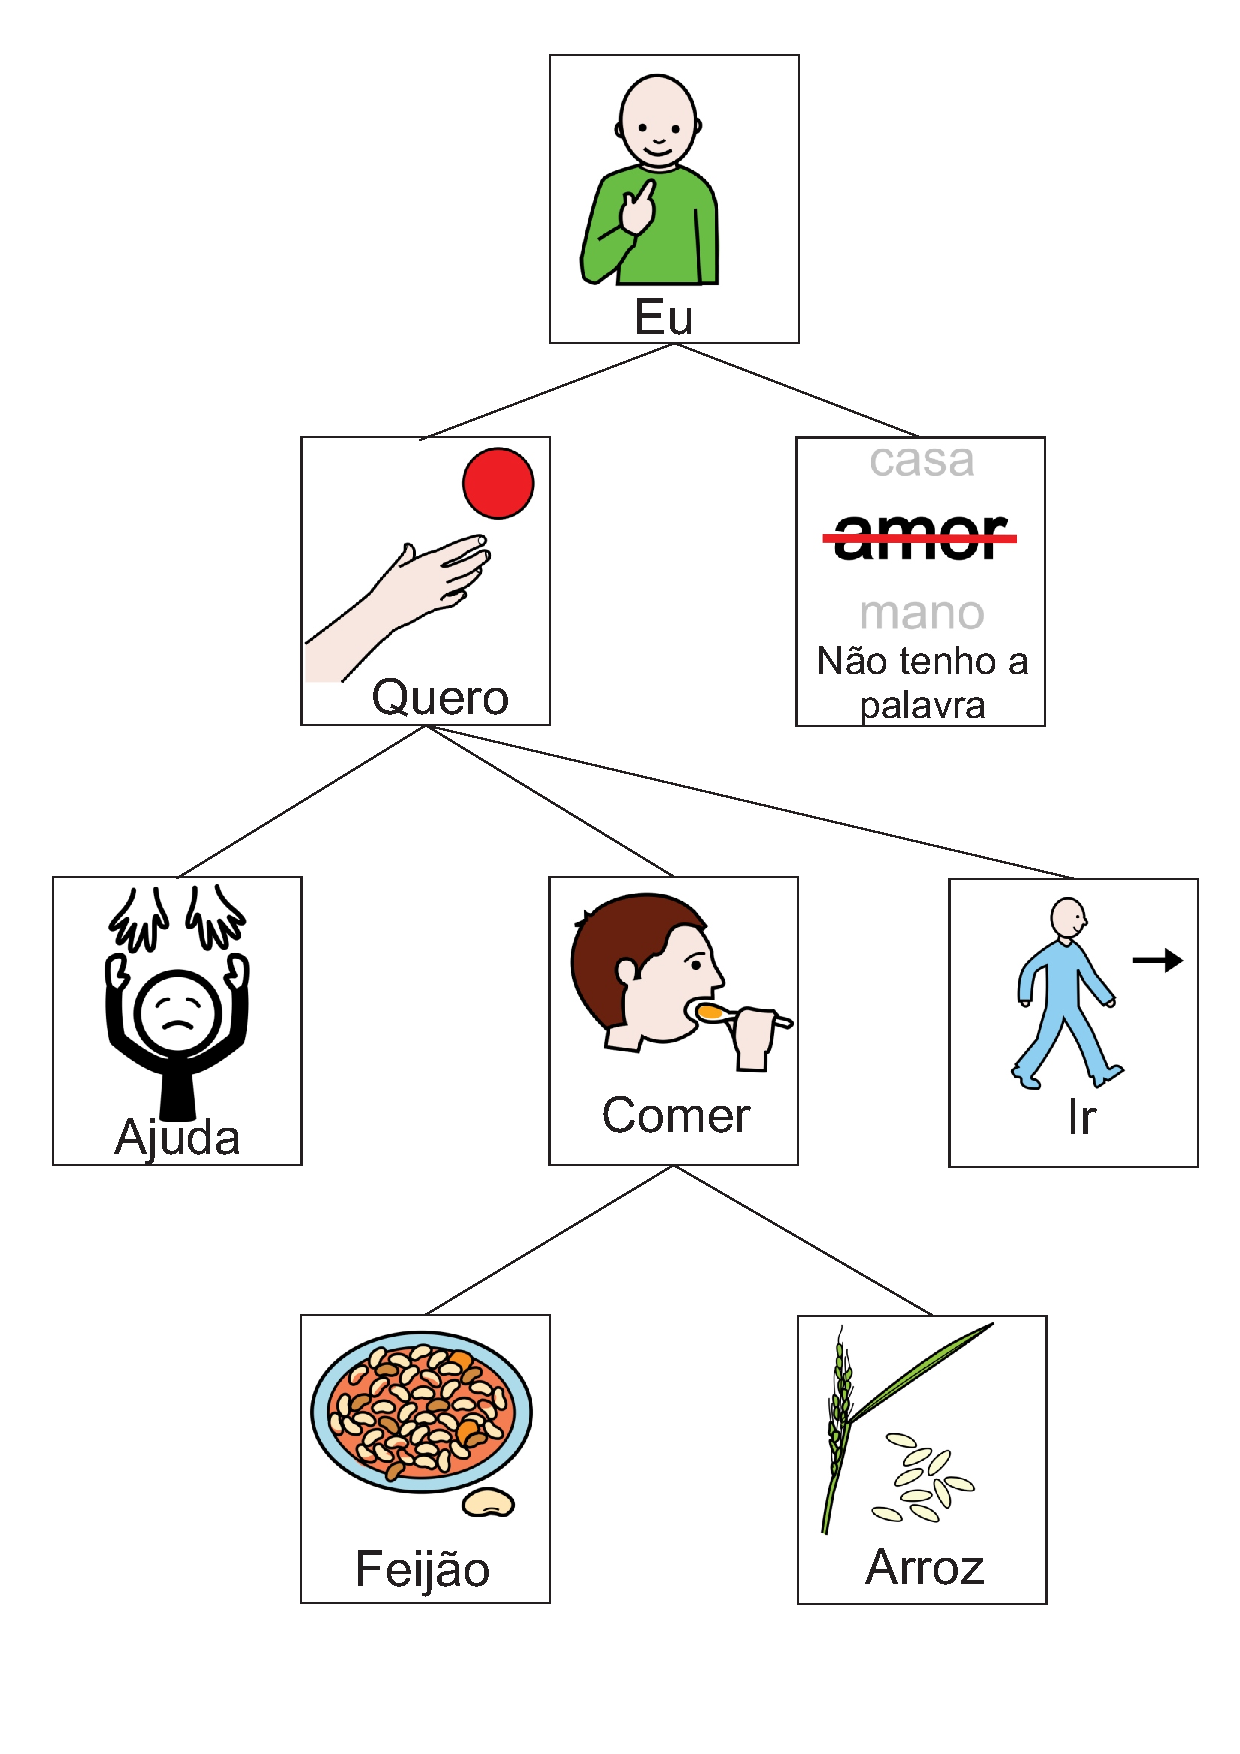
\includegraphics[width=6cm]{../figuras/arvore.pdf}\\
			Fonte: o pr�prio autor.
    \vspace{-1cm}
    \label{arvore}
  \end{center}
\end{figure}

A Figura \ref{arvore}, mesmo que contendo poucos pictogramas, ilustra a disposi��o dos pictogramas em �rvore que permite a forma��o de frases mais naturalmente, e reduz o n�mero de pictogramas, em rela��o a pictogramas com frases completas. Exemplo: o usu�rio clica no pictograma ``eu'', ap�s isso a solu��o vocaliza a palavra ``eu'', e apresenta na grade os dois pictogramas ``quero'' e ``n�o tenho a palavra'' e assim subsequentemente. Quando o usu�rio, excluir um pictograma, a solu��o ir� excluir todos os seus pictogramas relacionados, ou seja, seus filhos na �rvore.

O requisito n�o funcional n�mero um trata da perman�ncia de dados da solu��o, alguns m�todos podem ser citados, como banco de dados e grava��o em arquivos. Como o m�todo de grava��o em banco de dados, requer instala��o do banco de dados, e a vers�o e modelo do banco depender� da plataforma em que a solu��o executar�, para que a solu��o cumpra o requisito funcional n�mero seis e n�o funcional n�mero sete, o m�todo adotado ser� a grava��o de dados em arquivos. Para que haja uma melhor organiza��o dos dados, os arquivos ser�o utilizados no formato XML({\it eXtensible Markup Language}), que possuem suporte em Java a partir de \ac{APIS}.

O requisito n�o funcional n�mero dois, que diz respeito a disponibilidade, ser� cumprido ap�s a conclus�o do desenvolvimento da solu��o, quando ser� disponibilizado o projeto no ambiente {\it{Sourceforge}}\cite{sourceforge} que � um ambiente de disponibiliza��o de c�digos fontes, e projetos utilizados na Internet. O {\it{Sourceforge}} � um servi�o gratuito e � disponibilizado no endere�o http://sourceforge.net/.

Para que o usu�rio utilize a solu��o como foi planejada, a resolu��o da tela deve ser de 1366 x 768, que � padr�o de tela mais vendida nos computadores desktop \cite{monitor}. A sensibilidade ir� depender totalmente das interfaces que o usu�rio utilizar� (e.g., mouse inclusivo, aceler�metros e emuladores).

Para facilitar o compreendimento de satisfa��o dos requisitos, a tabela \ref{todos_requisitos} relaciona todos os requisitos (se��o \ref{req}) e como cada um foi cumprido nesta se��o. Sendo F. para os funcionais e N.F. n�o funcionais.
\begin{table}[bth!]
\centering
\scriptsize
\caption{Tabela de requisitos e de como s�o cumpridos}\vspace{.2cm}

 \begin{tabular}{ |p{2cm}|p{10.5cm}|p{3cm}|}
		
    \hline
		
    Tipo & Requisito & Solu��o proposta   \\ \hline \hline
		\multirow{8}{*}{Funcionais}& 1-A solu��o proposta deve apresentar uma grade de pictogramas & JFrame Java   \\ \cline{2-3} 
		&2-A solu��o deve aceitar diferentes formatos de s�mbolos e cores & \ac{APIS} Java \\ \cline{2-3}  
		&3-A solu��o deve aceitar s�mbolos criados pelo terapeuta & \ac{APIS} Java \\ \cline{2-3}  
		&4-Novos s�mbolos\- devem ser adicionados a grade \- sem que o usu�rio tenha \-experi�ncia no uso \-da solu��o & M�trica de usabilidade (Apreensibilidade) \\ \cline{2-3}   
		&5-A exclus�o de s�mbolos deve ser facilitada, ou seja, mesmo que a experi�ncia do usu�rio na solu��o seja pequena, ele deve conseguir realizar a tarefa & M�trica de usabilidade (Apreensibilidade) \\ \cline{2-3}   
		&6-A solu��o deve representar o que o usu�rio est� querendo expressar da melhor maneira poss�vel (e.g., entona��o, e pontua��o) & Google {\it Text-to-Speech}  \\ \cline{2-3}   
		&7-O usu�rio mesmo com defici�ncia deve conseguir apertar nos s�mbolos da solu��o & Metas de usabilidade  \\ \cline{2-3}   
		&8-Todos os s�mbolos devem ser acessados de uma forma simples, ou seja, sem categorias e arquiteturas complexas & Disposi��o de arquitetura de pictogramas em �rvore \\ \cline{2-3}   
		&9-Os s�mbolos devem ter tamanhos edit�veis & JFrame Java\\ \cline{2-3}   \hline
		\multirow{5}{*}{N�o Funcionais}&1-A solu��o tem que ser permanente, ou seja, guardar os s�mbolos e sua sequencia & Arquivos XML \\ \cline{2-3}
		&2-A solu��o deve estar dispon�vel e deve ser acess�vel a todas as pessoas, atrav�s do software disponibilizado em reposit�rios p�blicos & {\it Sourceforge} \\ \cline{2-3} 
		&3-O tempo de resposta da solu��o n�o deve causar frustra��o ao usu�rio, ou seja, a vocaliza��o da frase deve ser em um tempo menor a dois segundos & Google {\it Text-to-Speech}  \\ \cline{2-3} 
		&4-A utiliza��o da solu��o n�o deve depender do uso da internet & Grava��o de Arquivos de �udio \\ \cline{2-3} 
		&5-A licen�a da solu��o dever� permitir que outros pesquisadores possam aprimor�-la & Licen�a GPL \\ \cline{2-3} 
		&6-A solu��o deve estar em uma plataforma que aceite diferentes tipos de interface de entrada (e.g., mouse alternativo, aceler�metros e dispositivos espec�ficos de uma defici�ncia) & Java \\ \cline{2-3} \hline
		
    \end{tabular}
    \label{todos_requisitos}
		\vspace{0.3cm}
		\\Fonte: o pr�prio autor.

\end{table}

A tabela \ref{todos_requisitos} indica que foram encontrados m�todos para satisfazer todos os requisitos levantados. Apesar de todos os m�todos satisfazerem os requisitos, os m�todos possuem limita��es que s�o importantes mencionar.

\section{Limitadores}

Apesar da prancha de comunica��o, quando criada por Roxana Mayer Johnson em 1980 \cite{darcy}, ajudar no est�mulo de cogni��o e reabilita��o de outras tipos de defici�ncias (e.g., defici�ncia cerebral, autismo e crian�as sem defici�ncia), neste trabalho ser�o considerados apenas usu�rios com \ac{PC}, j� que outros tipos de defici�ncia tem condi��es espec�ficas n�o abordados no escopo do trabalho. Algumas outras limita��es da solu��o podem ser citadas:
\begin{enumerate}
\item  O trabalho n�o abordar� dispositivos de entradas alternativos (e.g., mouse inclusivo, aceler�metros e acionadores) que podem ser usados em conjunto com a solu��o, pois os dispositivos podem variar dependendo de do grau de \ac{PC} de cada usu�rio;
\item A escolha dos pictogramas e do paciente que usar� a solu��o ser� um papel desempenhado apenas pelo terapeuta, j� que estas escolhas dependem de fatores distintos n�o abordados neste trabalho (e.g., evolu��o, grau de les�o e percep��o);
\item Sobre a plataforma em que a solu��o estiver sendo executada; e
\begin{enumerate}
\item A mem�ria que ser� consumida por arquivos de �udio gravados pela solu��o para execu��es futuras, depender� da quantidade de mem�ria que a plataforma possui; e
\item A conex�o com a Internet � necess�ria para adicionar novos pictogramas a solu��o, por�m n�o � necess�ria para a utiliza��o de pictogramas previamente adicionados.
\end{enumerate}
\item N�o � poss�vel adicionar novos pictogramas sem o uso da Internet, devido a vocaliza��o depender da conex�o com o servi�o do Google.
\end{enumerate}

Sendo assim, os limitadores estar�o atrelados aos limitadores da plataforma em que a solu��o executa. Tamb�m � necess�rio que o terapeuta, escolha os seus pacientes de acordo com o grau de defici�ncia e sua evolu��o, para que a solu��o seja bem aproveitada.


\section{Plano de teste}
\label{testes}
Os testes da solu��o est�o divididos em tr�s etapas: Os testes internos, quando ser�o executados testes com docentes e discente da Universidade do Estado de Santa Catarina (UDESC), para a verifica��o das funcionalidade da solu��o. Os testes externos, que ser�o feitos com terapeutas das institui��es ACE e ADEJ, a fim de verificar as funcionalidades e a complexidade das tarefas com base em suas experi�ncias em rela��o a pessoas com \ac{PC}. Na terceira etapa ser�o feitos testes com pessoas que possuem \ac{PC}, a realiza��o destes testes ser�o feitos pelos terapeutas respons�veis por cada paciente, na inten��o de levantar n�o conformidades com a solu��o ao seu usu�rio final. Todas as etapas ser�o precedidas por um preenchimento do termo de consentimento conforme o anexo \ref{apendice2}. Como os usu�rios finais da solu��o possuem diferentes graus de \ac{PC}, evolu��o cognitiva e maturidade, n�o ser�o realizados testes em fun��o do tempo de realiza��o de cada tarefa. Algumas tarefas que foram consideradas principais de acordo com os requisitos determinados da solu��o ser�o testadas, s�o elas:


Tarefa n�mero um (Executar pictograma):
\vspace{-0.6cm}
\begin{enumerate}
\item{Abrir a solu��o;}
\item{Executar um pictograma previamente adicionado;}
\item{Escutar a vocaliza��o da frase; e}
\item{Voltar a grade principal.}
\end{enumerate}


Tarefa n�mero dois (Adicionar pictograma):
\vspace{-0.6cm}
\begin{enumerate}
\item{Adicionar um pictograma grade principal;}
\item{Atribuir uma frase ao pictograma;}
\item{Atribuir uma imagem ao pictograma; e}
\item{Escutar a vocaliza��o da frase.}
\end{enumerate}

Tarefa n�mero tr�s (Mudar o tamanho dos pictogramas):
\vspace{-0.6cm}
\begin{enumerate}
\item{Fechar a solu��o;}
\item{Abrir a solu��o;}
\item{Verificar se o pictograma adicionado na tarefa dois esta na grade principal; e}
\item{Mudar o tamanho dos s�mbolos da grade.}
\end{enumerate}

Tarefa n�mero quatro (Excluir Pictograma):
\vspace{-0.6cm}
\begin{enumerate}
\item{Excluir um pictograma;}
\item{Verificar se o pictograma foi exclu�do; e}
\item{Fechar a solu��o.}
\end{enumerate}

Ap�s a execu��o das tarefas, alguns itens ser�o avaliados em forma de um question�rio para medir a usabilidade, funcionalidade, efici�ncia e confiabilidade da solu��o. Os itens do question�rio (Tabela \ref{questionario}) foram baseados no \citeonline{rogers2002}, pois � amplamente utilizado na literatura.

\begin{table}[bth!]
\centering
\scriptsize
\caption{Question�rio}\vspace{.2cm}

    \begin{tabular}{ |p{2.5cm}|p{11.6cm}|l| }
		
    \hline
		
    Tarefa & Item  & Resposta  \\ \hline \hline
		\multirow{4}{*}{\parbox{2.5cm}{Tarefa um: Executar Pictograma}}& 1- Qual foi o grau de dificuldade encontrado na realiza��o da tarefa?\newline
		(Sendo 1 = f�cil, 2 = O.k., 3= dif�cil ou 4 = precisou de ajuda) &   \\ \cline{2-3}
		 & 2- Os passos da tarefa estavam claros?\newline
		(Sendo 1 = f�cil, 2 = O.k., 3= dif�cil ou 4 = precisou de ajuda) &   \\ \cline{2-3}
		 & 3- Quantos erros foram cometidos na realiza��o da tarefa? &   \\ \cline{2-3}
		 & 4- Ap�s a realiza��o da tarefa o objetivo foi cumprido?\newline
		(Sendo 1 = Totalmente Cumprido, 2= Apenas Parcialmente, 3 = N�o foi cumprida.) &   \\ \cline{2-3} \hline 
		\multirow{4}{*}{\parbox{2.5cm}{Tarefa dois: Adicionar Pictograma}}& 1- Qual foi o grau de dificuldade encontrado na realiza��o da tarefa?\newline
		(Sendo 1 = f�cil, 2 = O.k., 3= dif�cil ou 4 = precisou de ajuda) &   \\ \cline{2-3}
		 & 2- Os passos da tarefa estavam claros?\newline
		(Sendo 1 = f�cil, 2 = O.k., 3= dif�cil ou 4 = precisou de ajuda) &   \\ \cline{2-3}
		 & 3- Quantos erros foram cometidos na realiza��o da tarefa?  &   \\ \cline{2-3}
		 & 4- Ap�s a realiza��o da tarefa o objetivo foi cumprido? \newline
		(Sendo 1 = Totalmente Cumprido, 2= Apenas Parcialmente, 3 = N�o foi cumprida.) &   \\ \cline{2-3} \hline
	\multirow{4}{*}{\parbox{2.5cm}{Tarefa tr�s: Mudar o tamanho dos Pictogramas}}& 1- Qual foi o grau de dificuldade encontrado na realiza��o da tarefa?\newline
	  (Sendo 1 = f�cil, 2 = O.k., 3= dif�cil ou 4 = precisou de ajuda) &   \\ \cline{2-3}
		 & 2- Os passos da tarefa estavam claros? \newline
		(Sendo 1 = f�cil, 2 = O.k., 3= dif�cil ou 4 = precisou de ajuda) &   \\ \cline{2-3}
		 & 3- Quantos erros foram cometidos na realiza��o da tarefa?  &   \\ \cline{2-3}
		 & 4- Ap�s a realiza��o da tarefa o objetivo foi cumprido?\newline
		(Sendo 1 = Totalmente Cumprido, 2= Apenas Parcialmente, 3 = N�o foi cumprida.) &   \\ \cline{2-3} \hline
		\multirow{4}{*}{\parbox{2.5cm}{Tarefa quatro: Excluir Pictograma}}& 1- Qual foi o grau de dificuldade encontrado na realiza��o da tarefa?\newline (Sendo 1 = f�cil, 2 = O.k., 3= dif�cil ou 4 = precisou de ajuda) &   \\ \cline{2-3}
		 & 2- Os passos da tarefa estavam claros? \newline
		(Sendo 1 = f�cil, 2 = O.k., 3= dif�cil ou 4 = precisou de ajuda) &   \\ \cline{2-3}
		 & 3- Quantos erros foram cometidos na realiza��o da tarefa?  &   \\ \cline{2-3}
		 & 4- Ap�s a realiza��o da tarefa o objetivo foi cumprido?\newline
		(Sendo 1 = Totalmente Cumprido, 2= Apenas Parcialmente, 3 = N�o foi cumprida.) &   \\ \cline{2-3} \hline

    \end{tabular}
    \label{questionario}
		\vspace{0.3cm}
		Fonte: o pr�prio autor.
		

\end{table}

Ap�s cada fase as notas dos question�rios ser�o contabilizadas, e as tarefas ser�o revistas se classificadas como:
\begin{itemize}
\item Item 1 - ``Dif�cil'' ou ``precisou de ajuda'';
\item Item 2 - ``Dif�cil'' ou ``precisou de ajuda'';
\item Item 3 - maior que 0; e
\item Item 4 - ``apenas parcialmente'' ou ``n�o foi cumprida''.
\end{itemize}

Como trata-se de uma pesquisa qualitativa, o fechamento amostral ocorrer� por crit�rios de sele��o, ou seja, a satura��o da amostra, � feita por um processo cont�nuo da an�lise de dados coletados, e este processo � feito at� o momento que pouco de substancialmente novo aparece\cite{amostra}. No contexto do trabalho, ser� considerado a satura��o da amostra, no momento que haja no m�ximo um ponto de varia��o na m�dia, para cada categoria. Na primeira fase de testes, os testes internos, ser�o realizados com usu�rios que possuem os seguintes crit�rios de sele��o:

\begin{itemize}
\item Docentes e Discente da \ac{UDESC};
\item Conhecimento ou experi�ncia;
\begin{itemize}
\item na �rea de \acf{TA}; e/ou 
\item na �rea de Engenharia de Software.
\end{itemize}
\item Conhecimento em inform�tica; e
\item Conhecimento de como funciona uma prancha de comunica��o.
\end{itemize}

Na segunda fase de testes, ser�o feitos os mesmos testes com o question�rio \ref{questionario} com, psic�logos e terapeutas, que j� utilizam a solu��o prancha de comunica��o com seus pacientes, com o prop�sito de encontrar n�o conformidades com a solu��o. Por fim na terceira fase, ser�o refeitos os teste com os mesmos terapeutas e psic�logos, ap�s o uso da solu��o junto aos seus pacientes, para que os psic�logis e terapeutas apontem problemas e sugiram melhoras da solu��o.


\section{Estrutura da Solu��o}

A estrutura da solu��o � feita de modo hier�rquico porque � considerada mais simples e desde que a organiza��o hier�rquica n�o seja muito profunda, esta estrutura favorece a cria��o de um modelo mental de navega��o por parte dos usu�rios \cite{goncalves}. A estrutura de modo hier�rquico foi escolhida tamb�m para manter o padr�o da solu��o, j� que os pictogramas est�o tamb�m organizados da mesma forma. A estrutura � aconselhada para usu�rios principiantes, e � caracterizada por organizar o fluxo de tarefas de modo hier�rquico (ou em �rvore), respeitando um fluxo �nico e comum desde a tarefa principal at� as tarefas que dela dependem hierarquicamente e assim sucessivamente. Isto �, do topo para a base, as informa��es v�o sendo detalhadas atrav�s de v�rios n�veis uma vez que, de cada tarefa secund�ria, podem sair m�ltiplas liga��es para outras tarefas de n�vel inferior na hierarquia\cite{goncalves}. A Figura \ref{estrutura} representa a estrutura da solu��o e suas tarefas.


\begin{figure}[bth!]
  \begin{center}
    \caption{Estrutura da solu��o}\vspace{.4cm}
			
      \centering
      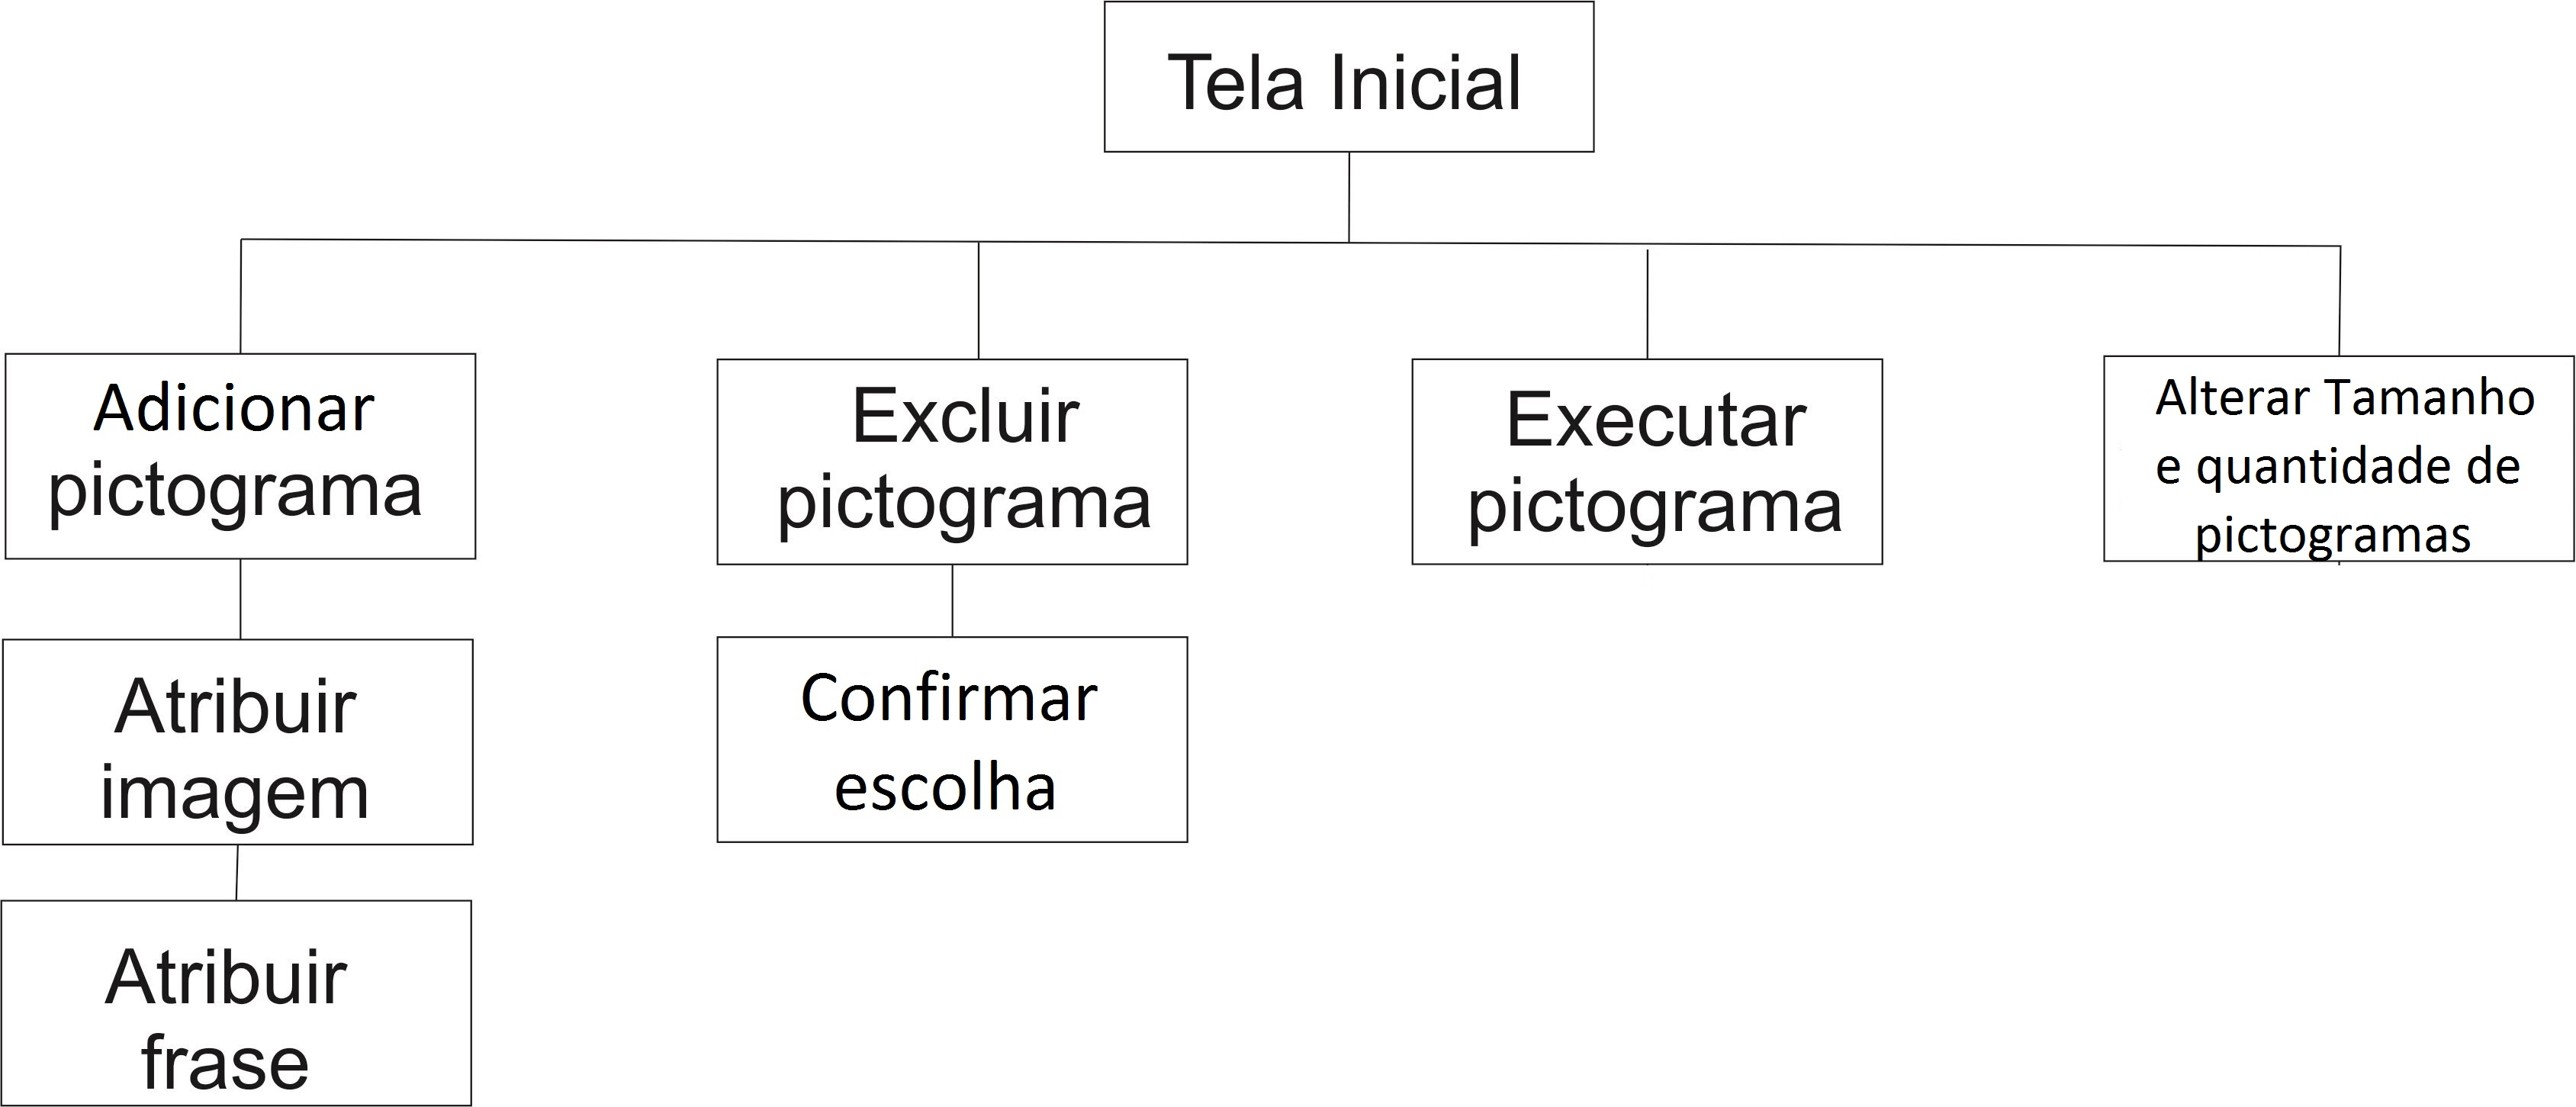
\includegraphics[scale=0.6]{../figuras/estrutura.jpg}\\
			Fonte: o pr�prio autor.
    
    \label{estrutura}
  \end{center}
\end{figure}

A Figura \ref{estrutura} ilustra as principais tarefas do programa e sua disposi��o. A disposi��o das tarefas em modo hier�rquico auxilia a meta de usabilidade no quesito de facilidade de aprendizagem, pois respeita um fluxo �nico de informa��es ao navegar a solu��o.



\section{Prot�tipo}
\label{prototipo}

Ap�s feito a especifica��o da proposta, foi elaborado um prot�tipo de baixa fidelidade\footnote{Prot�tipos de baixa fidelidades, s�o prot�tipos da representa��o art�stica da solu��o com detalhes omissos do funcionamento.}, com a finalidade de encontrar recursos faltantes no projeto te�rico. A Figura \ref{layout} representa o prot�tipo da tela inicial da solu��o.

\begin{figure}[bth!]
  \begin{center}
    \caption{Prot�tipo}
			
      \centering
      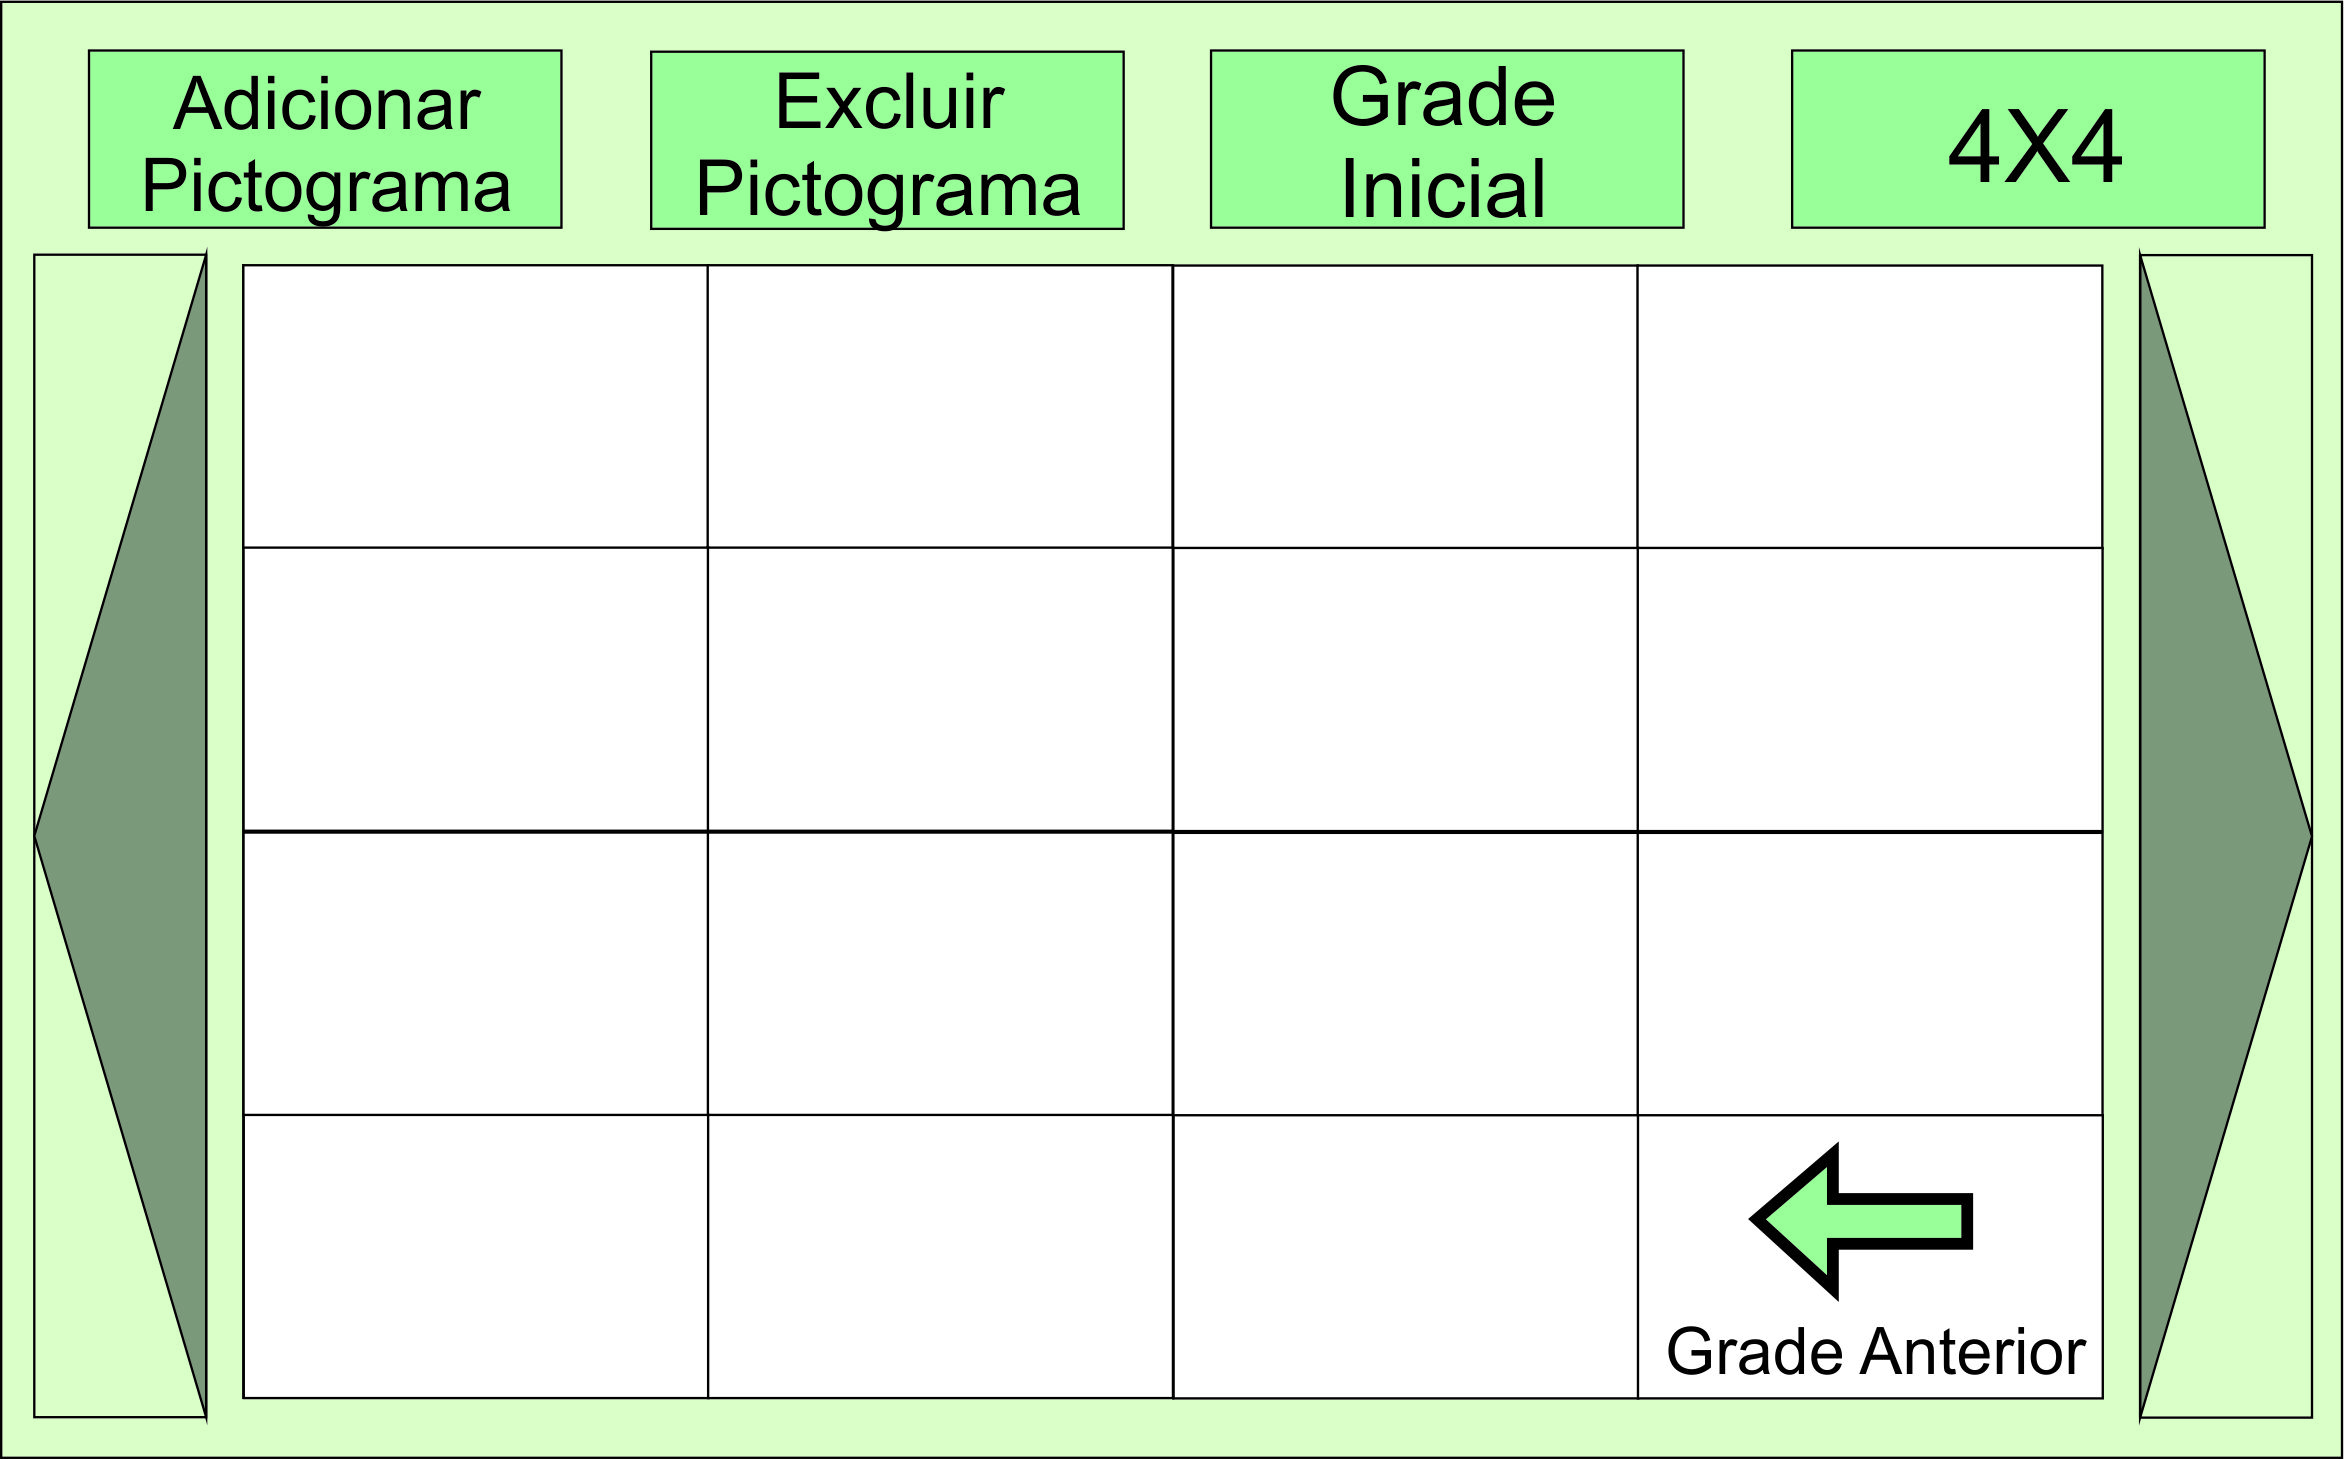
\includegraphics[scale=0.6]{../figuras/layout.jpg}\\
			Fonte: o pr�prio autor.
    
    \label{layout}
  \end{center}
\end{figure}
\vspace{-0.4cm}

A Figura \ref{layout} representa um prot�tipo da solu��o. Na parte superior foram adicionado quatro bot�es, s�o eles, ``Adicionar Pictograma'', ``Excluir Pictograma'', ``Grade Inicial'' e ``4X4''. Os bot�es possuem as seguintes funcionalidades:
\begin{itemize}
\item O bot�o ``Adicionar Pictograma'', � referente a tarefa de adicionar um pictograma ao n� atual, n�o definido anteriormente ;
\item O bot�o ``Excluir Pictograma'', � referente a tarefa excluir pictograma, do n� atual e apagar suas informa��es como �udio e imagem, al�m disso a solu��o exclui as informa��es dos pictogramas relacionados ao pictograma exclu�do;
\item O bot�o ``Grade Inicial'', faz com que a grade apresente os pictogramas do primeiro n� da �rvore de pictogramas mencionada na se��o \ref{esp}; e
\item O bot�o ``4X4'' � referente a troca de tamanhos dos pictogramas na grade, ele representa a quantidade de pictogramas atualmente na grade.
\end{itemize}
Os bot�es adicionados nas laterais, representando flechas para esquerda e direita, s�o para a navega��o de bot�es relacionados ao n� anterior caso, a lista de bot�es relacionados seja maior que a quantidade de bot�es apresentada atualmente na grade. O bot�o no lado inferior direito, com a legenda de grade anterior, � para que o usu�rio possa subir um n�vel na �rvore de pictogramas. Exemplificando, com o tamanho da grade 4x4 os 15 bot�es em branco retangulares ao centro, s�o onde v�o ficar os pictogramas da solu��o.

\section{Diagrama de Classes}
\label{funcao}
Com base nos requisitos e interface, foram definidas as principais classes com seus m�todos e atributos da solu��o. A Figura \ref{diagrama_classes} representa o diagrama de classes da solu��o proposta.

\begin{figure}[bth!]
  \begin{center}
    \caption{Diagrama de Classes}
			
      \centering
      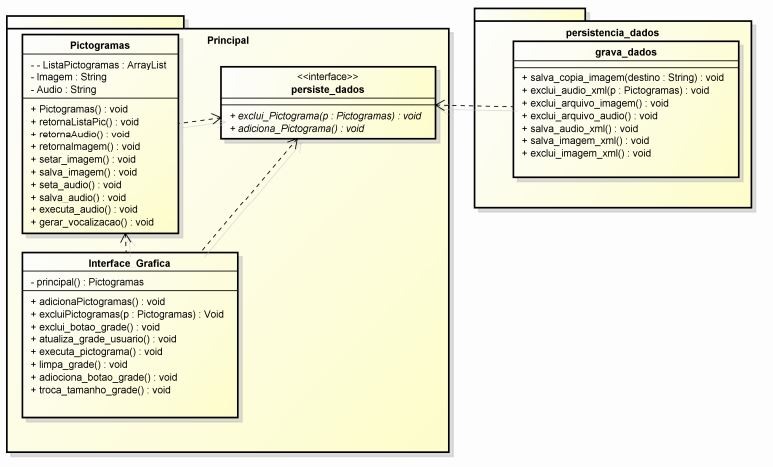
\includegraphics[scale=0.8]{../figuras/diagrama_classe.jpg}\\
			\vspace{0.15cm}
			Fonte: o pr�prio autor.
    \vspace{0.15cm}
    \label{diagrama_classes}
  \end{center}
\end{figure}

A solu��o cont�m 31 fun��es divididas em quatro grupos, a classe pictograma, Interface\_gr�fica, grava\_dados e persiste\_dados. As fun��es da classe pictograma s�o:

\begin{itemize}
\item Pictogramas() : Fun��o construtura, que invoca as fun��es setar\_imagem(), gere\_vocaliza��o e seta\_audio();

\item retornaListaPic : A fun��o retorna os Pictogramas relacionados ao objeto;

\item retornaAudio : A fun��o retorna o caminho do arquivo de �udio relacionado ao objeto;

\item retornaImagem : A fun��o retorna o caminho do arquivo de Imagem relacionado ao objeto;

\item setarImagem: Atribui ao Objeto o caminho da Imagem relacionada;

\item salvaImagem: Salva c�pia da imagem na pasta da solu��o;

\item seta\_audio: Atribui ao Objeto o caminho do �udio relacionado; 

\item executaAudio: executa o arquivo de �udio relacionado ao objeto;

\item gerar\_vocalizacao: Se conecta com a m�quina {\it Text-to-Speech} do Google para receber arquivo de �udio e usa a fun��o setar\_audio() para gravar o caminho do arquivo; e

\item salva\_pictograma: invoca a fun��o salva\_pictograma da interface persiste\_dados.

\end{itemize}

As fun��es da classe Interface\_Grafica s�o:
\begin{itemize}
\item adicionaPictogramas :  instancia um novo pictograma atrav�s do construtor Pictograma();

\item excluiPictogramas : invoca a fun��o da interface persiste\_dados exclui\_Pictogramas();

\item trocaTamanho : troca a quantidade de bot�es na grade da solu��o;

\item exclui\_botao\_grade : retira pictograma da grade da solu��o;

\item atualiza\_grade\_usuario : redesenha a grade da solu��o para o usu�rio quando h� uma modifica��o;

\item executa\_pictograma : executa o arquivo de �udio atribu�do ao pictograma;

\item limpa\_grade: retira todos os bot�es da grade da solu��o; e

\item adiciona\_botao\_grade : adiciona um novo bot�o na grade.

\end{itemize}

As fun��es da classe grava\_dados s�o:

\begin{itemize}
\item salva\_copia\_imagem: salva c�pia do arquivo de imagem em uma pasta pr�-selecionada;

\item exclui\_audio\_xml: exclui no arquivo XML o caminho do �udio referente ao pictograma;

\item exclui\_imagem\_xml: exclui no arquivo XML o caminho da imagem referente ao pictograma;

\item exclui\_arquivo\_imagem: exclui a c�pia do arquivo de imagem referente ao pictograma;

\item exclui\_arquivo\_audio: exclui arquivo de �udio referente ao pictograma;

\item salva\_audio\_xml: salva em arquivo XML o caminho do �udio referente ao pictograma;

\item salva\_imagem\_xml: salva em arquivo XML o caminho da imagem referente ao pictograma

\item salva\_Pictograma: invoca as fun��es: salva\_copia\_imagem(), salva\_audio\_xml() e salva\_imagem\_xml(); e

\item exclui\_Pictograma: invoca as fun��es: exclui\_audio\_xml, exclui\_imagem\_xml, exclui\_arquivo\_imagem e exclui\_arquivo\_audio.

\end{itemize}

As fun��es da interface persiste\_dados como s�o fun��es de uma interface n�o implementam nenhum tipo de c�digo:
\begin{itemize}
\item salva\_Pictograma; e

\item exclui\_Pictograma.
\end{itemize}


Definidas as fun��es � necess�rio definir as intera��es do usu�rio com a solu��o, com base na exce��o das tarefas padr�es que se espera do sistema. Al�m disso, a defini��o das tarefas permite identificar se o diagrama de classe � satisfeito.

\section{Diagramas das Tarefas}
\label{diagramas}
Para melhor compreens�o das tarefas da solu��o, ap�s a descri��o da solu��o e de como cada requisito ser� cumprido foram definidos os casos de uso, diagramas de sequ�ncia e sequ�ncia de telas para cada tarefa da solu��o. As tarefas descritas s�o:
\begin{itemize}
\item Incluir Pictograma;
\item Excluir Pictograma;
\item Alterar Tamanho dos pictogramas na grade; e 
\item Executar Pictogram.
\end{itemize}

Essas tarefas foram consideradas principais na solu��o de acordo com os requisitos levantados. Para maior compreens�o foi elaborado diagramas e sequ�ncias de telas que explicam a intera��o do usu�rio em cada tarefa.

\subsection{Tarefa Incluir Pictograma}

Ap�s definir os m�todos para satisfa��o dos requisitos, foi descrita a tarefa de incluir pictograma. A Figura \ref{caso_incluir} representa o caso de uso da tarefa incluir pictograma.
\vspace{-0.3cm}
\begin{figure}[bth!]
  \begin{center}
    \caption{Caso de uso incluir pictograma}

      \centering
      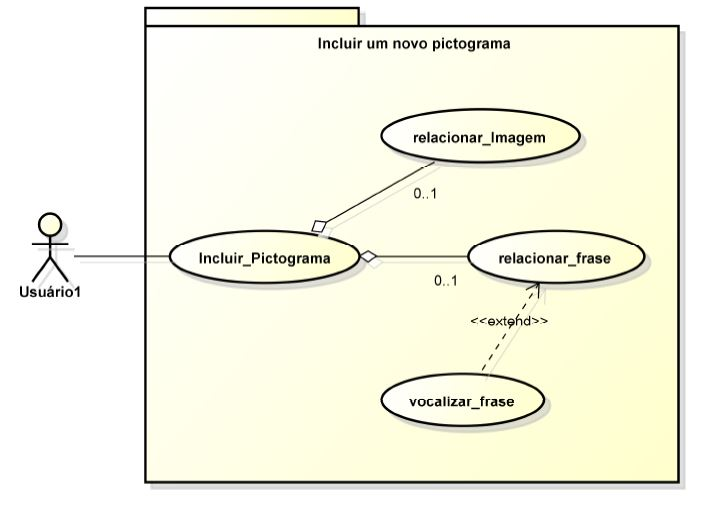
\includegraphics[scale=0.5]{../figuras/caso_incluir.jpg}\\

			Fonte: o pr�prio autor.
   \vspace{-1cm}
    \label{caso_incluir}
  \end{center}
\end{figure}


O caso de uso da tarefa incluir pictograma definido na Figura \ref{caso_incluir}, se reflete no diagrama de sequ�ncia da figura \ref{sequencia_adiciona}. Para a elabora��o do diagrama de sequ�ncia foram usadas as fun��es descritas na se��o \ref{funcao}.

\begin{figure}[bth!]
  \begin{center}
    \caption{Diagrama de sequ�ncia da tarefa incluir pictograma}
			\vspace{1cm}
      \centering
      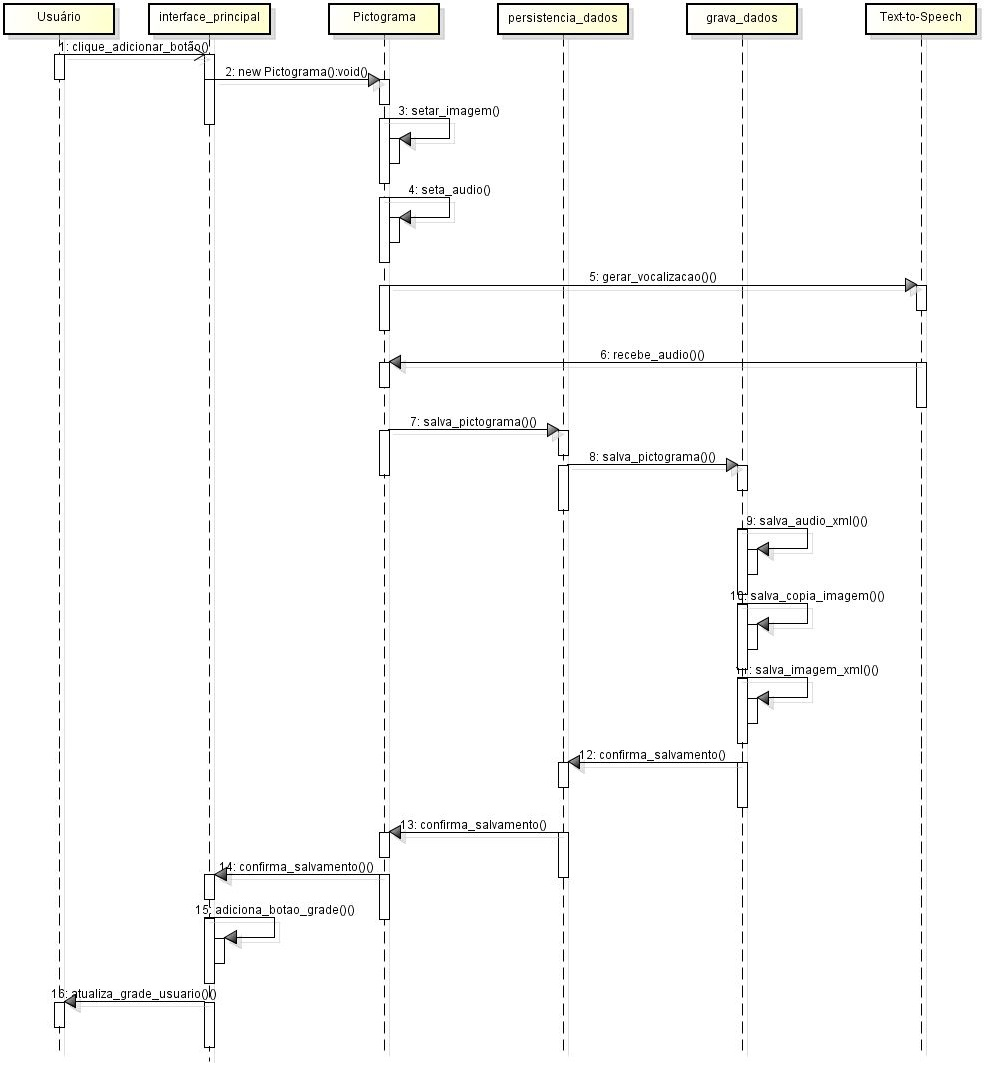
\includegraphics[scale=0.68]{../figuras/sequencia_adiciona.jpg}\\
			\vspace{0.3cm}
			Fonte: o pr�prio autor.
    \vspace{0.3cm}
    \label{sequencia_adiciona}
  \end{center}
\end{figure}

Para melhor compreens�o foi elaborado uma sequ�ncia de telas representadas por passos nas Figuras \ref{adiciona_1}, \ref{adiciona_2}, \ref{adiciona_3} e \ref{adiciona_4} que representam a tarefa incluir pictograma e os eventos realizados pelo usu�rio para concluir a tarefa. 


\begin{figure}[ht] 
  \label{agrup_adicionar} 
  \begin{minipage}[b]{0.5\linewidth}
    \centering
		\caption{Passo um} 
    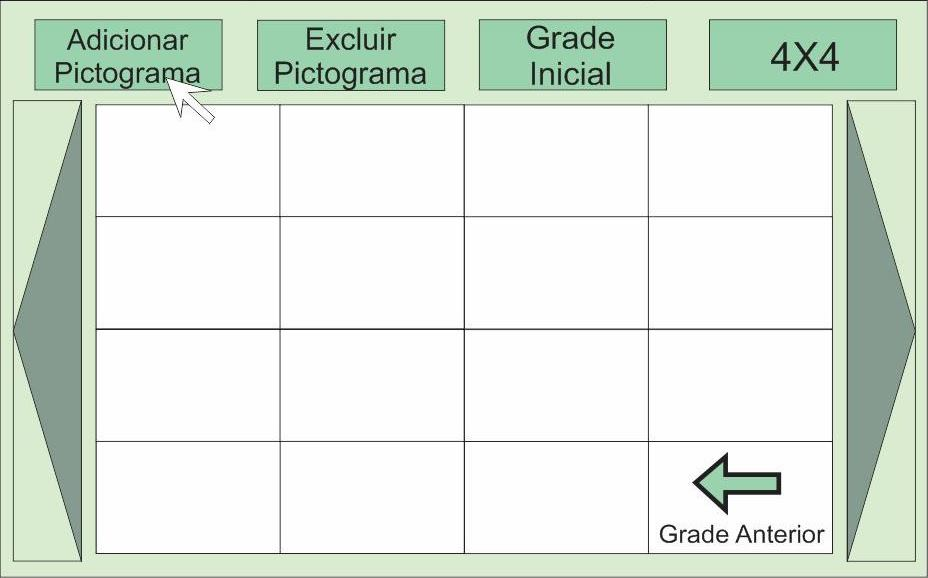
\includegraphics[width=1\linewidth]{../figuras/Adicionar/1.jpg} 
		\label{adiciona_1}
	
  \end{minipage} %%
  \begin{minipage}[b]{0.5\linewidth}
    \centering
		\caption{Passo dois} 
    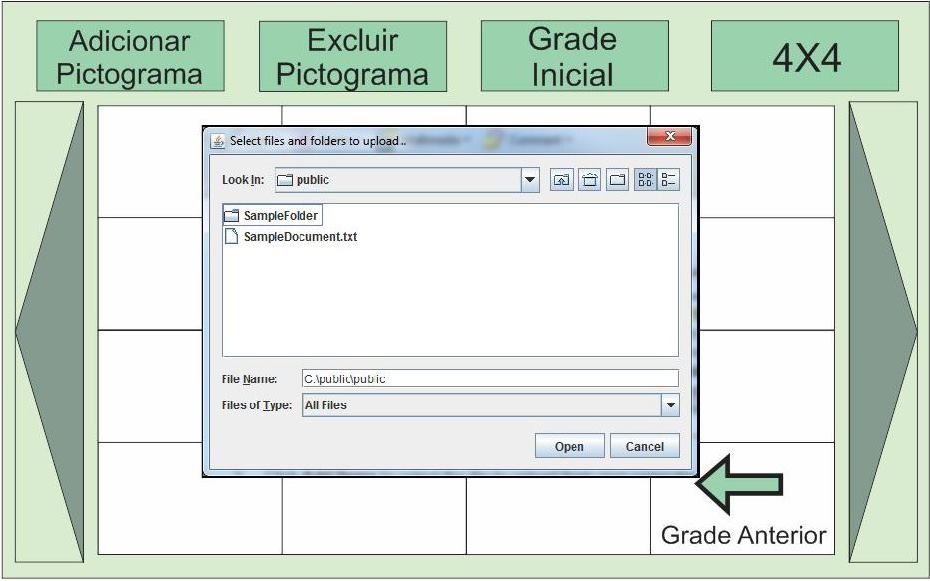
\includegraphics[width=1\linewidth]{../figuras/Adicionar/2.jpg} 
		\label{adiciona_2}
	
  \end{minipage} %% 
  \begin{minipage}[b]{0.5\linewidth}
    \centering
		\caption{Passo tr�s} 
    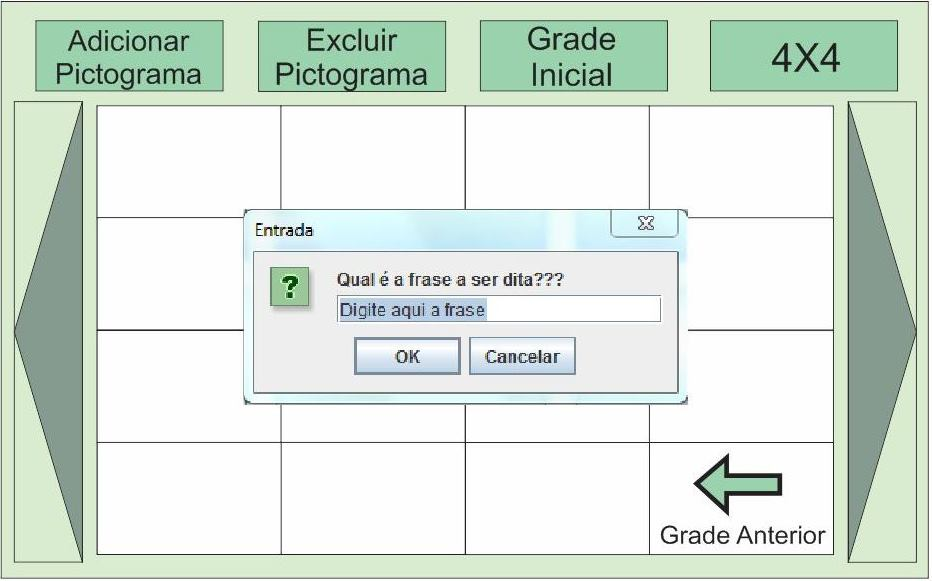
\includegraphics[width=1\linewidth]{../figuras/Adicionar/3.jpg} 
		\label{adiciona_3}

  \end{minipage} %% 
  \begin{minipage}[b]{0.5\linewidth}
    \centering
		\caption{Passo quatro} 
    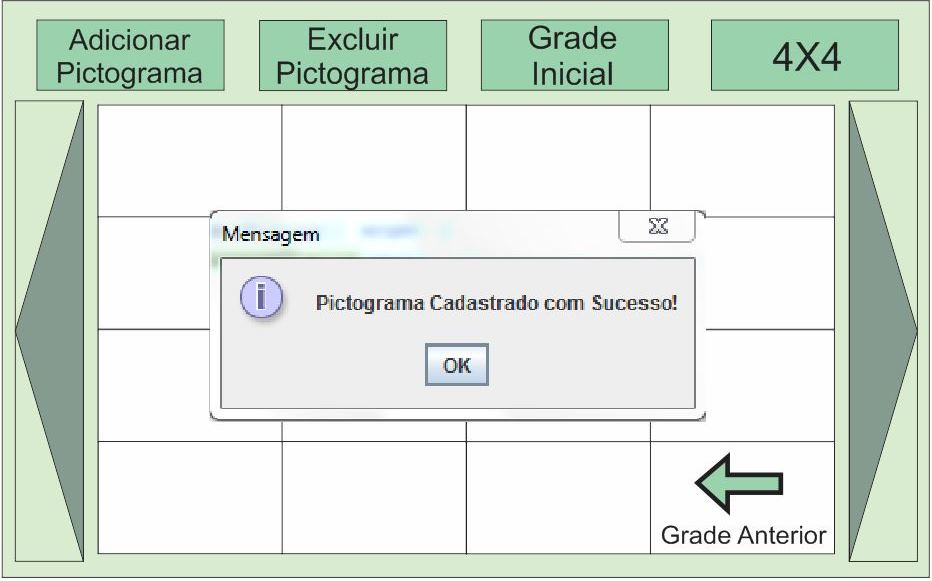
\includegraphics[width=1\linewidth]{../figuras/Adicionar/4.jpg} 
		\label{adiciona_4}

  \end{minipage} %% 
	\center{Fonte: pr�prio autor.}
\end{figure}

O passo um (Figura \ref{adiciona_1}) representa o clique do mouse do usu�rio no bot�o Adicionar Pictograma. Percebe-se que � feito, atrav�s do movimento do cursor inicialmente, podendo ser reconfigurado por teclas de atalho. O passo dois (Figura \ref{adiciona_2}) consiste no usu�rio escolher a imagem relacionada ao pictograma, atrav�s de uma caixa de escolha de arquivos na plataforma do usu�rio. No passo tr�s (Figura \ref{adiciona_3}) o usu�rio ir� inserir o texto que ele deseja ser vocalizado quando o pictograma for executado. Por fim, o passo quatro (Figura \ref{adiciona_4}) � a resposta ao usu�rio de que o pictograma foi adicionado com sucesso.

\subsection{Tarefa Executar Pictograma}

A tarefa principal da solu��o � a tarefa de executar os pictogramas. A Figura \ref{caso_executar} representa o caso de uso da tarefa executar um pictograma.
\vspace{0.5cm}

\begin{figure}[bth!]
  \begin{center}
    \caption{Caso de uso da execu��o de um pictograma}
			
      \centering
      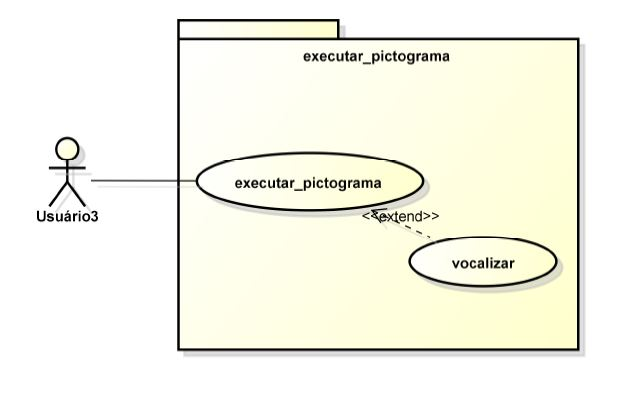
\includegraphics[scale=0.5]{../figuras/caso_executar.jpg}\\
			Fonte: o pr�prio autor.
    
    \label{caso_executar}
  \end{center}
\end{figure}

A Figura \ref{sequencia_executa} representa o diagrama de sequ�ncia da tarefa executar um pictograma refletida pelo seu caso de uso. Na defini��o do diagrama de sequ�ncia foi usada as fun��es definidas na se��o \ref{funcao}.

\begin{figure}[bth!]
  \begin{center}
    \caption{Diagrama de sequ�ncia da execu��o de um pictograma}
      \centering
      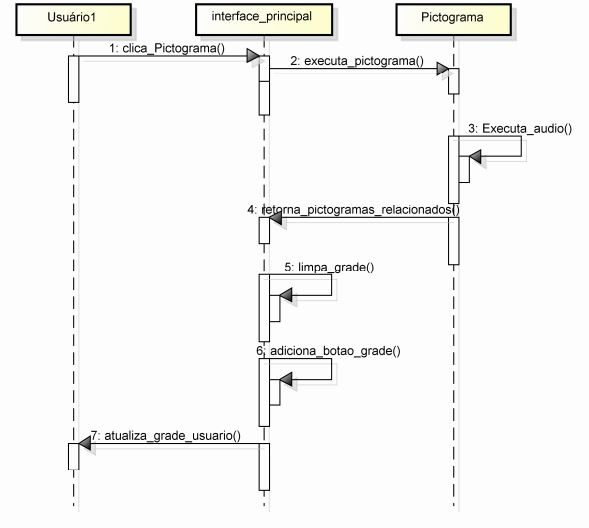
\includegraphics[scale=0.7]{../figuras/sequencia_executa.jpg}\\
			Fonte: o pr�prio autor.
    
    \label{sequencia_executa}
  \end{center}
\end{figure}

Para o melhor compreendimento foi feito uma sequ�ncia de passos representados pelas Figuras \ref{executar_1} e \ref{executar_2} que representam de executar um pictograma e os eventos realizados pelo usu�rio para concluir a tarefa.
\vspace{1cm}
\begin{figure}[ht] 
  \label{agrup_executar} 
  \begin{minipage}[b]{0.5\linewidth}
    \centering
		\caption{Passo um} 
    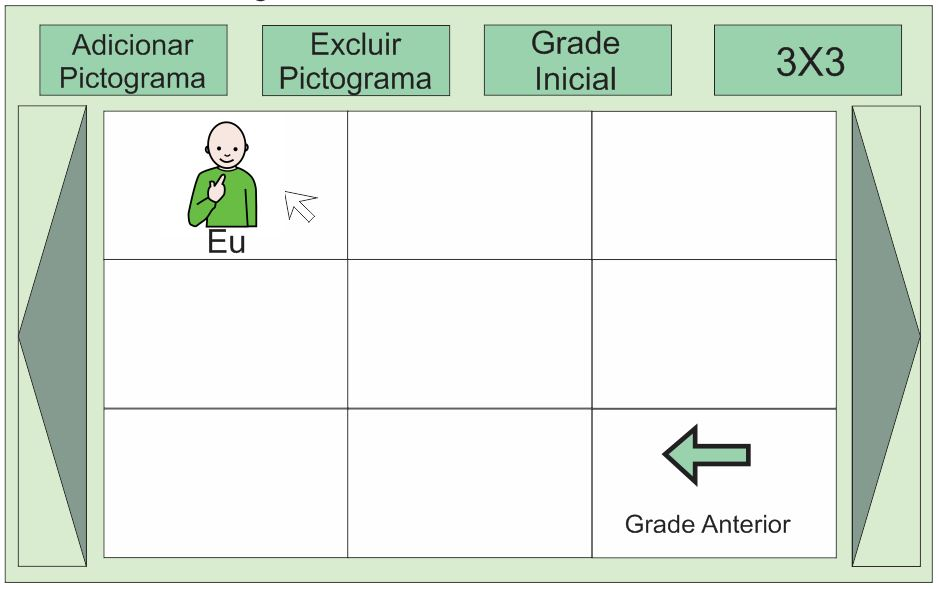
\includegraphics[width=1\linewidth]{../figuras/Executar/1.jpg} 
		\label{executar_1}
		\vspace{-1cm}
  \end{minipage}%%
  \begin{minipage}[b]{0.5\linewidth}
    \centering
		\caption{Passo dois} 
    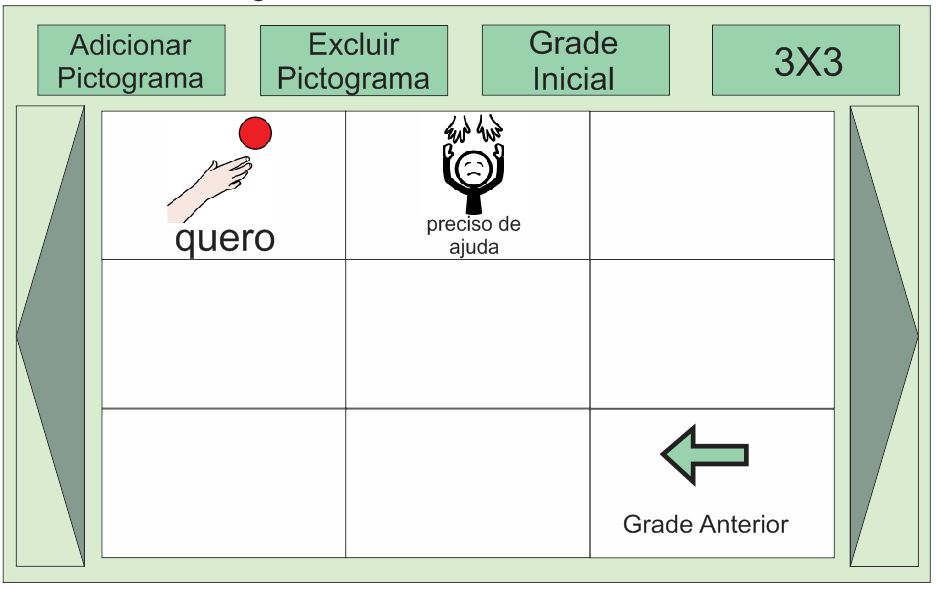
\includegraphics[width=1\linewidth]{../figuras/Executar/2.jpg} 
		\label{executar_2}
		\vspace{-1cm}
  \end{minipage} %% 
		\vspace{-1cm}
	\center{Fonte: pr�prio autor.}
\end{figure}

O passo (Figura \ref{executar_1}) um representa o clique do usu�rio no pictograma ``EU''. Ap�s o clique, a solu��o vocalizar� a palavra ``EU'' e apresentar� seus pictogramas relacionados representados no passo dois (Figura \ref{executar_2}), e a tarefa estar� conclu�da. 


\subsection{Tarefa Alterar Tamanho dos Pictogramas na Grade}

Como o tamanho dos bot�es devem ser edit�veis, a tarefa alterar tamanho dos pictogramas � necess�ria. A Figura \ref{caso_tamanho} representa o caso de uso da tarefa alterar o tamanho dos pictogramas na grade.

\begin{figure}[bth!]
  \begin{center}
    \caption{Caso de troca de tamanhos dos pictogramas}
			
      \centering
      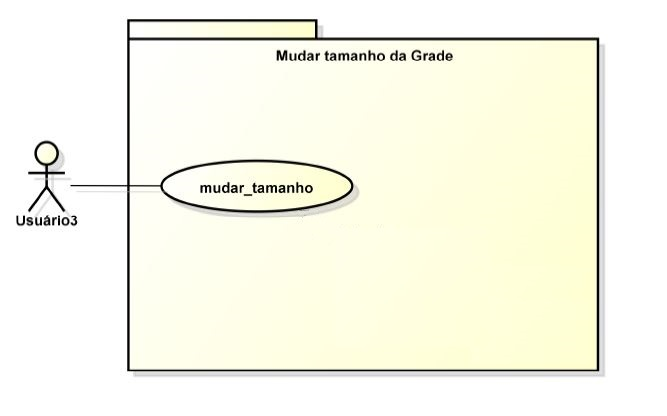
\includegraphics[scale=0.4]{../figuras/caso_tamanho.jpg}\\
			Fonte: o pr�prio autor.
    
    \label{caso_tamanho}
  \end{center}
\end{figure}

A Figura \ref{sequencia_tamanho} representa o diagrama de sequ�ncia da tarefa alterar o tamanho dos pictogramas na grade. Na defini��o do diagrama de sequ�ncia foram empregadas fun��es definidas na se��o \ref{funcao}.

\begin{figure}[bth!]
  \begin{center}
    \caption{Diagrama de sequ�ncia de troca de tamanhos dos pictogramas}
			\vspace{0.2cm}
      \centering
      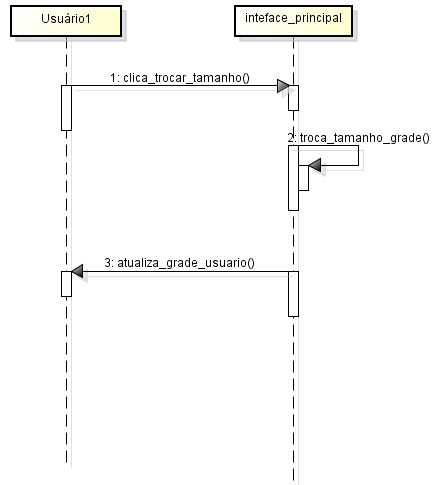
\includegraphics[scale=0.6]{../figuras/sequencia_tamanho.jpg}\\
				\vspace{-0.3cm}
			Fonte: o pr�prio autor.
    \vspace{-0.5cm}
    \label{sequencia_tamanho}
  \end{center}
\end{figure}

Para o melhor compreendimento foi feito uma sequ�ncia de passos representados pelas Figuras \ref{troca_1}, \ref{troca_2} e \ref{troca_3}, que representam a tarefa alterar tamanho dos pictogramas na grade e os eventos realizados pelo usu�rio para concluir a tarefa.
\vspace{-0.4cm}
\begin{figure}[ht] 
  \label{agrup_troca} 
  \begin{minipage}[b]{0.5\linewidth}
    \centering
		\caption{Passo um} 
    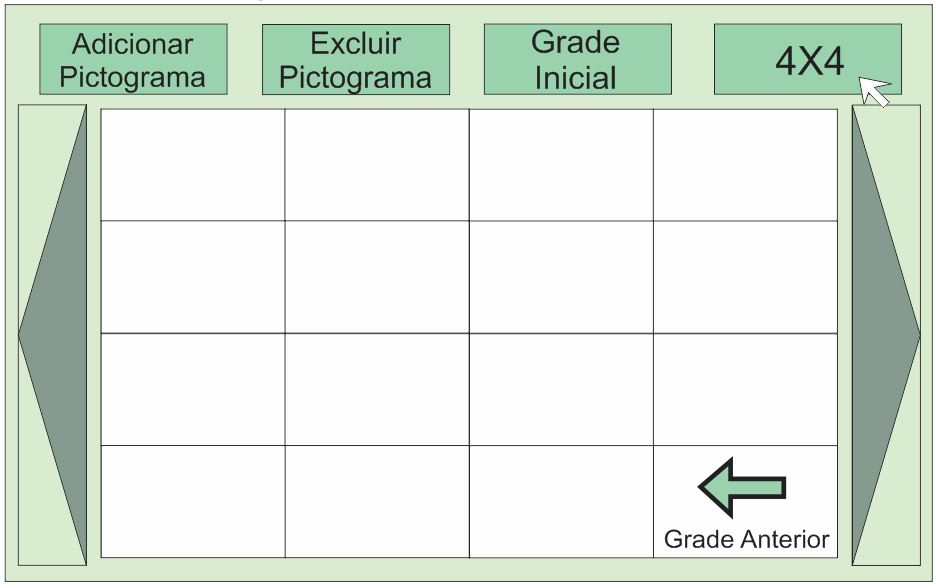
\includegraphics[width=1\linewidth]{../figuras/Troca/1.jpg} 
		\label{troca_1}
		\vspace{-1.0cm}
  \end{minipage}%%
  \begin{minipage}[b]{0.5\linewidth}
    \centering
		\caption{Passo dois} 
    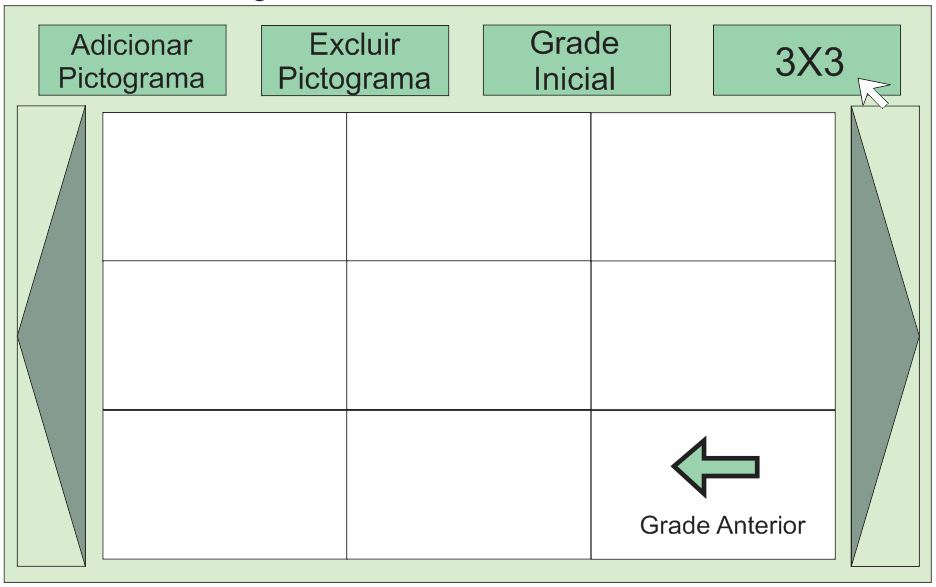
\includegraphics[width=1\linewidth]{../figuras/Troca/2.jpg} 
		\label{troca_2}
		\vspace{-1.0cm}
  \end{minipage} %% 
  \begin{minipage}[b]{0.5\linewidth}
    \centering
		\caption{Passo tr�s} 
    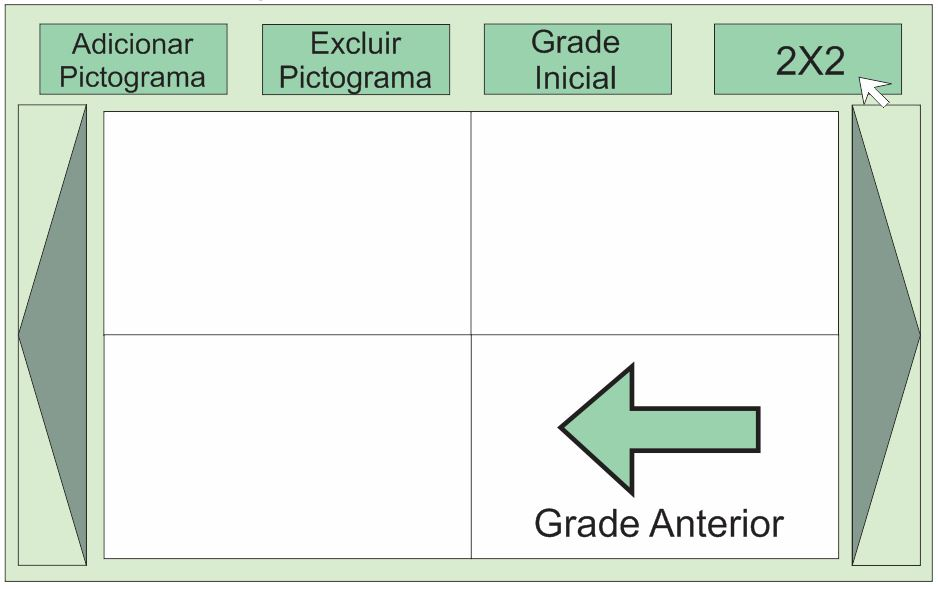
\includegraphics[width=1\linewidth]{../figuras/Troca/3.jpg} 
		\label{troca_3}
		\vspace{-1.1cm}
  \end{minipage}%% 
	\vspace{-0.4cm}
	\center{Fonte: pr�prio autor.}
	\vspace{-2cm}
\end{figure}

\vspace{2cm}
O passo um (Figura \ref{troca_1}) representa o clique do usu�rio no bot�o ``4X4''. A solu��o mudar� a quantidade e tamanho de bot�es na tela e apresentar� a configura��o demonstrada no passo dois. O passo dois (Figura \ref{troca_2}) representa um clique do usu�rio no bot�o ``3X3'' , a solu��o mudar� novamente a quantidade e tamanho de bot�es na tela e apresentar� a configura��o demonstrada no passo tr�s (Figura \ref{troca_3}), caso o usu�rio clique no bot�o ``2X2'' a solu��o voltar� a mostrar a configura��o do passo um.


	
\subsection{Tarefa Excluir Pictograma}

Ap�s definir os m�todos para satisfa��o dos requisitos, foi descrita a tarefa de excluir um pictograma. A Figura \ref{caso_excluir} representa o caso de uso da tarefa excluir pictograma. 
\begin{figure}[bth!]
  \begin{center}
    \caption{Caso de uso da tarefa excluir pictograma}
		\vspace{1cm}
			
      \centering
      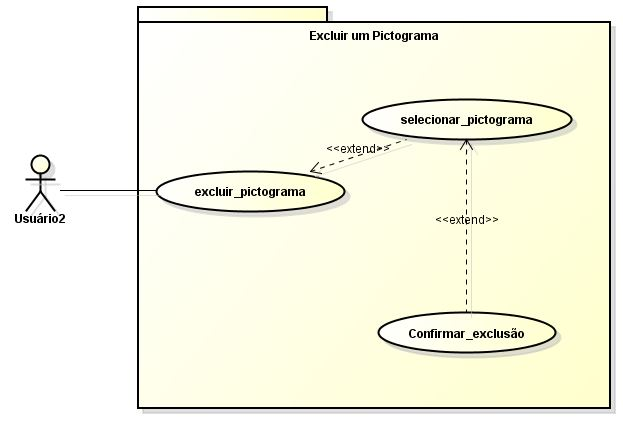
\includegraphics[scale=0.7]{../figuras/caso_excluir.jpg}\\
			
			Fonte: o pr�prio autor.
			
    
    \label{caso_excluir}
  \end{center}
\end{figure}

Ap�s definido o caso de uso da tarefa incluir pictograma, definido na Figura \ref{caso_excluir}, foi definido o diagrama de sequ�ncia da tarefa incluir pictograma representada pela Figura \ref{sequencia_excluir}. Na defini��o do diagrama de sequ�ncia foram usada fun��es definidas na se��o \ref{funcao}.
\vspace{3cm}

\begin{figure}[bth!]
  \begin{center}
    \caption{Diagrama de sequencia da tarefa excluir pictograma}
			
      \centering
      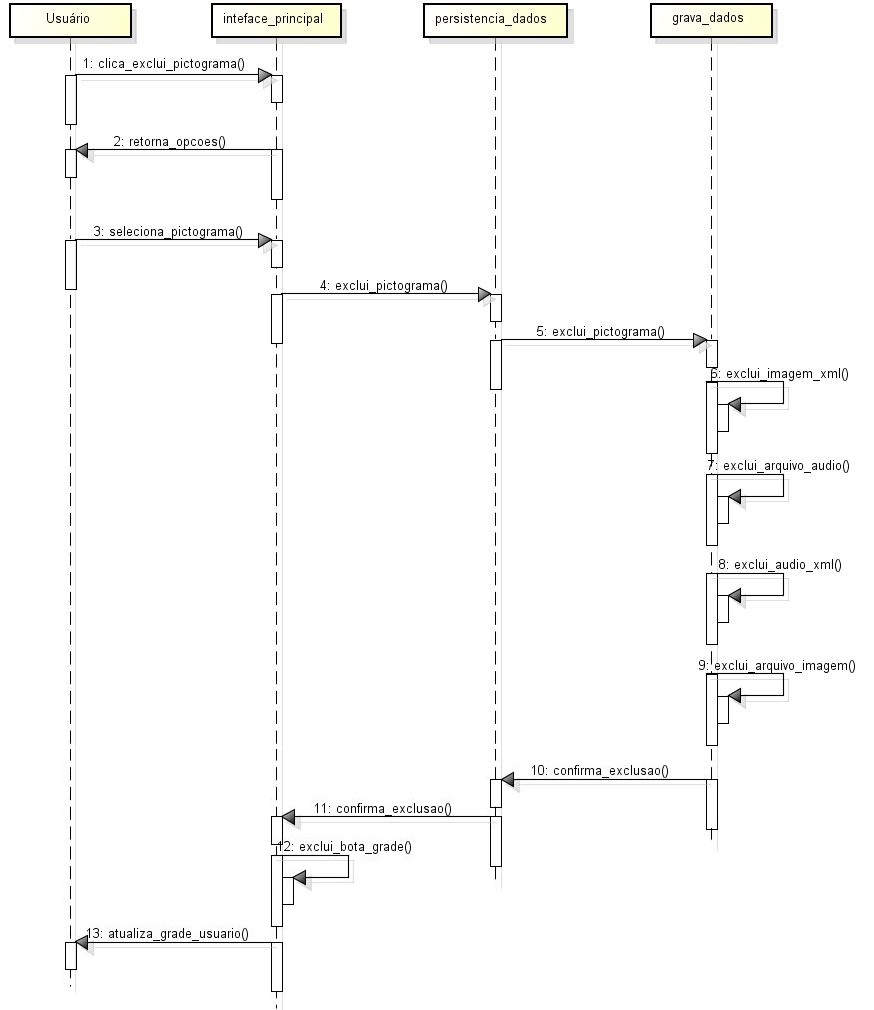
\includegraphics[scale=0.75]{../figuras/sequencia_exclui.jpg}\\
			
			Fonte: o pr�prio autor.
			
    
    \label{sequencia_excluir}
  \end{center}
\end{figure}


Para o melhor compreendimento foi elaborado uma sequ�ncia de passos representados pelas figuras \ref{exclui_1}, \ref{exclui_2}, \ref{exclui_3}, \ref{exclui_4} e \ref{exclui_5}. As figuras representam a tarefa excluir pictograma e os eventos realizados pelo usu�rio para concluir a tarefa.

\vspace{2cm}
\begin{figure}[ht] 
  \label{agrup_excluir} 
  \begin{minipage}[b]{0.5\linewidth}
    \centering
		\caption{Passo um} 
    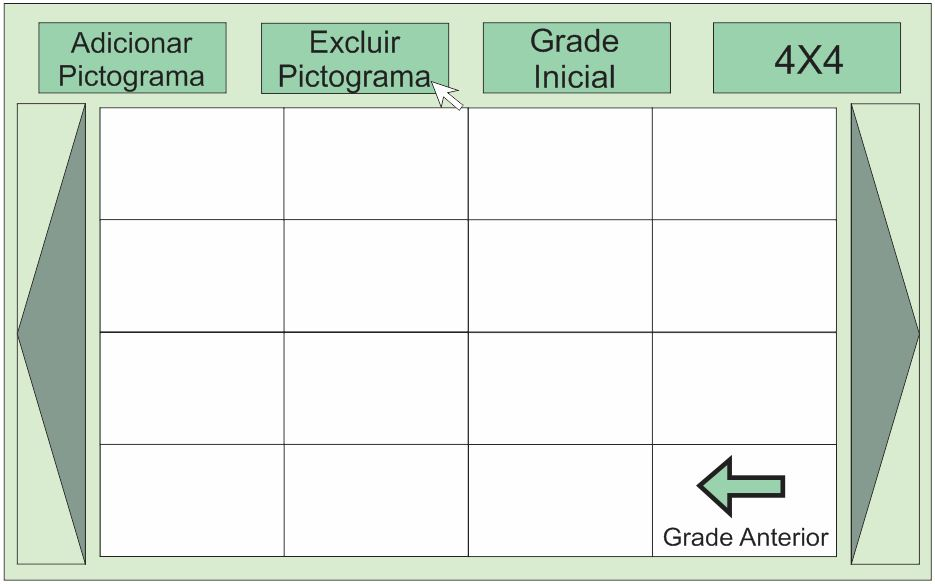
\includegraphics[width=1\linewidth]{../figuras/Excluir/1.jpg} 
		\label{exclui_1}
		\vspace{-1cm}
  \end{minipage} %%
  \begin{minipage}[b]{0.5\linewidth}
    \centering
		\caption{Passo dois} 
    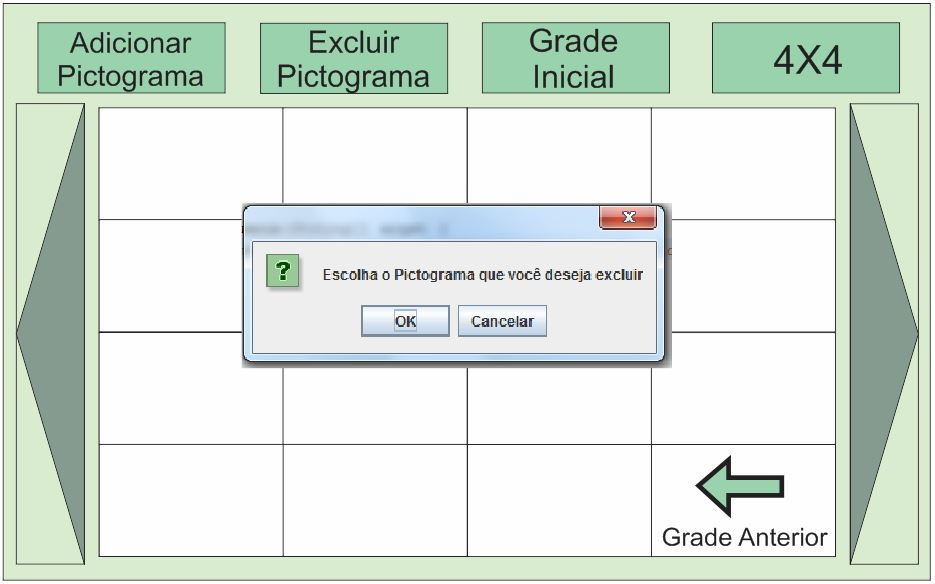
\includegraphics[width=1\linewidth]{../figuras/Excluir/2.jpg} 
		\label{exclui_2}
		\vspace{-1cm}
  \end{minipage} %% 
  \begin{minipage}[b]{0.5\linewidth}
    \centering
		\caption{Passo tr�s} 
    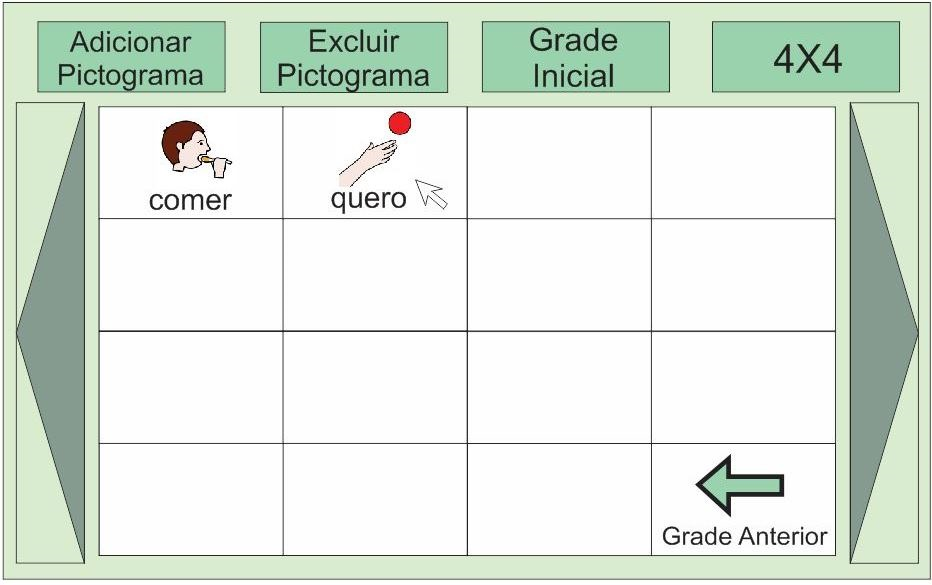
\includegraphics[width=1\linewidth]{../figuras/Excluir/3.jpg} 
		\label{exclui_3}
		\vspace{-1cm}
  \end{minipage} %% 
  \begin{minipage}[b]{0.5\linewidth}
    \centering
		\caption{Passo quatro} 
    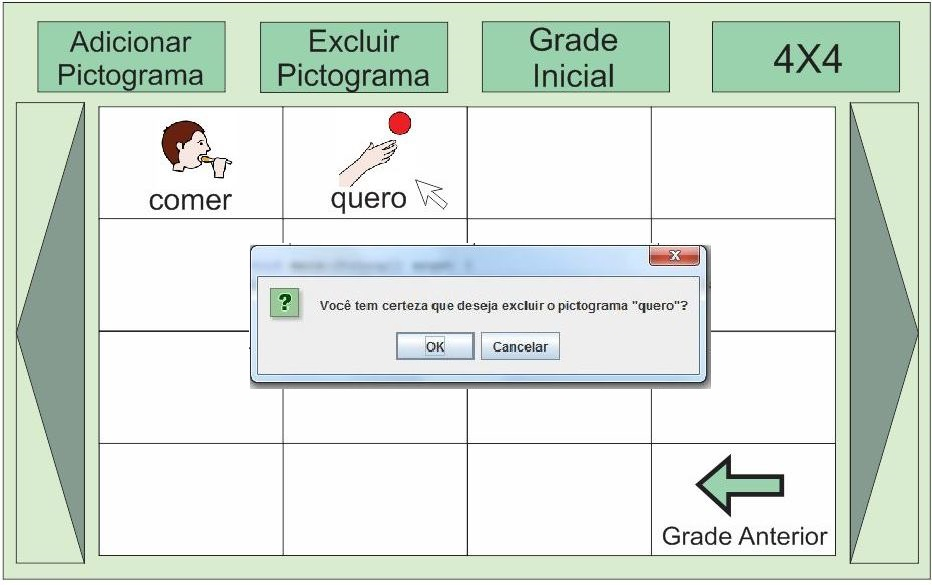
\includegraphics[width=1\linewidth]{../figuras/Excluir/4.jpg} 
		\label{exclui_4}
		\vspace{-1cm}
  \end{minipage} %% 
	\begin{minipage}[b]{0.5\linewidth}
    \centering
		\caption{Passo cinco} 
    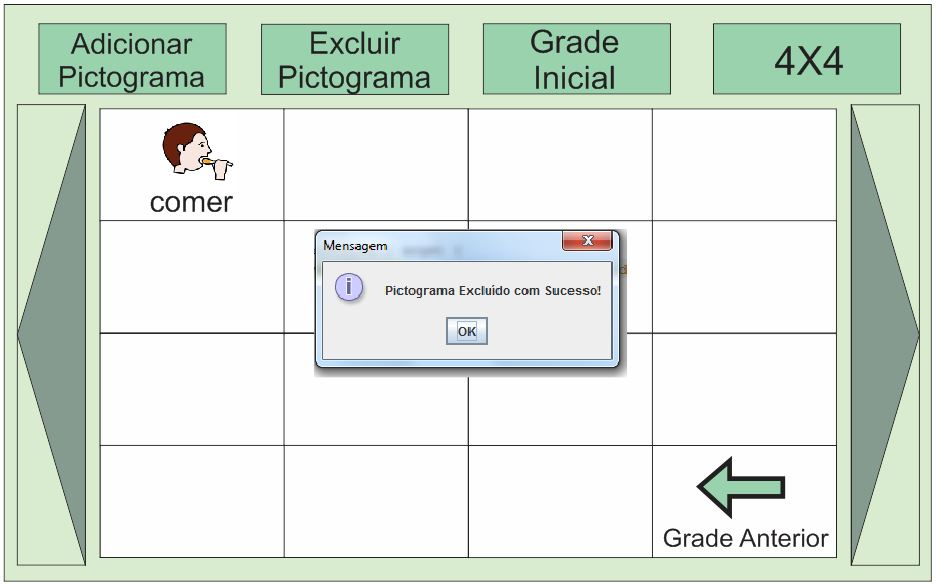
\includegraphics[width=1\linewidth]{../figuras/Excluir/5.jpg} 
		\label{exclui_5}
		\vspace{-1cm}
  \end{minipage} %% 
	\center{Fonte: pr�prio autor.}
\end{figure}

O passo um (Figura \ref{exclui_1}) representa o clique do mouse do usu�rio no bot�o Excluir pictograma, atrav�s de movimentos do cursor. O passo dois (Figura \ref{exclui_2}) consiste na solu��o informar o pr�ximo passo ou dar op��o de cancelar a tarefa caso o usu�rio tenha apertado o bot�o por engano. No passo tr�s (Figura \ref{exclui_3}) o usu�rio ir� selecionar o pictograma a ser exclu�do. No passo quatro (Figura \ref{exclui_4}) a solu��o confirma se o usu�rio deseja realmente excluir o pictograma selecionado. O passo cinco (Figura \ref{exclui_5}) representa um {\it feedback} ao usu�rio de que o pictograma foi exclu�do com sucesso. Conclu�das as defini��es das tarefas e o papel do usu�rio em cada uma delas, a solu��o pode ser representada pelo seu atual estado em um diagrama de estados.

\section{Diagrama de Estados}

Ap�s definido os casos de uso e diagramas de sequ�ncia da solu��o, afim de definir os estados da solu��o no decorrer da execu��o dos processos, foi elaborado um diagrama de estados da solu��o representado pela Figura \ref{diagrama_estados}. O diagrama representa as entradas de dados feitas pelos usu�rios e as a��es realizadas pela solu��o.
\vspace{-0.4cm}
\begin{figure}[bth!]
  \begin{center}
    \caption{Diagrama de estados}
      \centering
      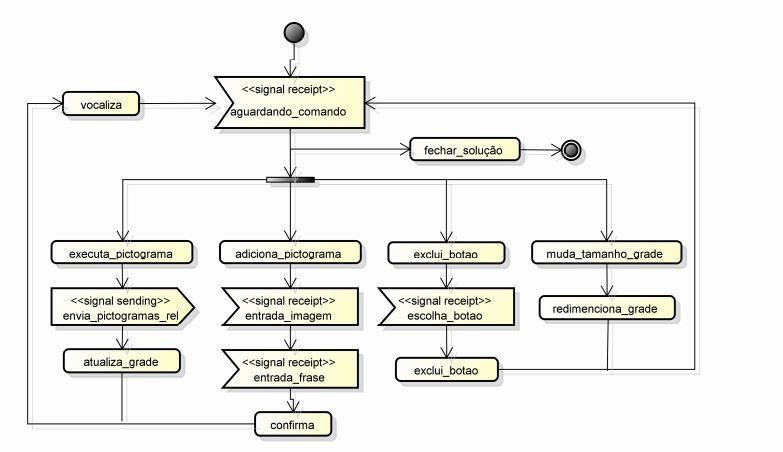
\includegraphics[scale=0.6]{../figuras/diagrama_estados.jpg}\\
			\vspace{-0.3cm}
			Fonte: o pr�prio autor.
    \vspace{-0.9cm}
    \label{diagrama_estados}
  \end{center}
\end{figure}

A Figura \ref{diagrama_estados} ilustra as intera��es do usu�rio nas caixas de {\it signal receipt}, e as demais caixas representam as a��es da solu��o. O in�cio e o fim da execu��o s�o marcados por c�rculos pretos, o fim com uma aur�ola preta ao redor do c�rculo.

\section{Considera��es do Cap�tulo}

Os requisitos possibilitaram uma solu��o limpa e objetiva, que facilitam o uso da solu��o tanto por pessoas com \ac{PC} como pelo seu terapeuta. Os testes foram descritos afim de encontrar n�o conformidades com a solu��o e tornar a solu��o com alta simplicidade nas tarefas, tendo sempre em mente que o usu�rio final � uma pessoa que possui \ac{PC}.

A estrutura da solu��o, assim como, os casos de uso e itera��es do usu�rio, s�o realizados com base nas diretrizes de usabilidade descritas na se��o \ref{esp}, afim da solu��o ser facilmente memorizada e aprendida, eficiente, objetiva e principalmente que haja um conforto e aceitabilidade do usu�rio ao utiliz�-la. Por fim, o cap�tulo no seu total, tem como objetivo especificar a solu��o e as itera��es do usu�rio, e principalmente constatar a sua viabilidade.

\chapter{Implementa��o e Testes}
\label{cap:captestes}

Durante todo o desenvolvimento da solu��o foram utilizadas as orienta��es e diagramas do cap�tulo \ref{cap:proposta}. A solu��o
foi baseada no prot�tipo desenhado na sec��o \ref{prototipo}. A figura \ref{fig:solucao} representa a solu��o implementada.

\begin{figure}[bth!]
  \begin{center}
    \caption{A solu��o implementada}\vspace{.2cm}
			
      \centering
      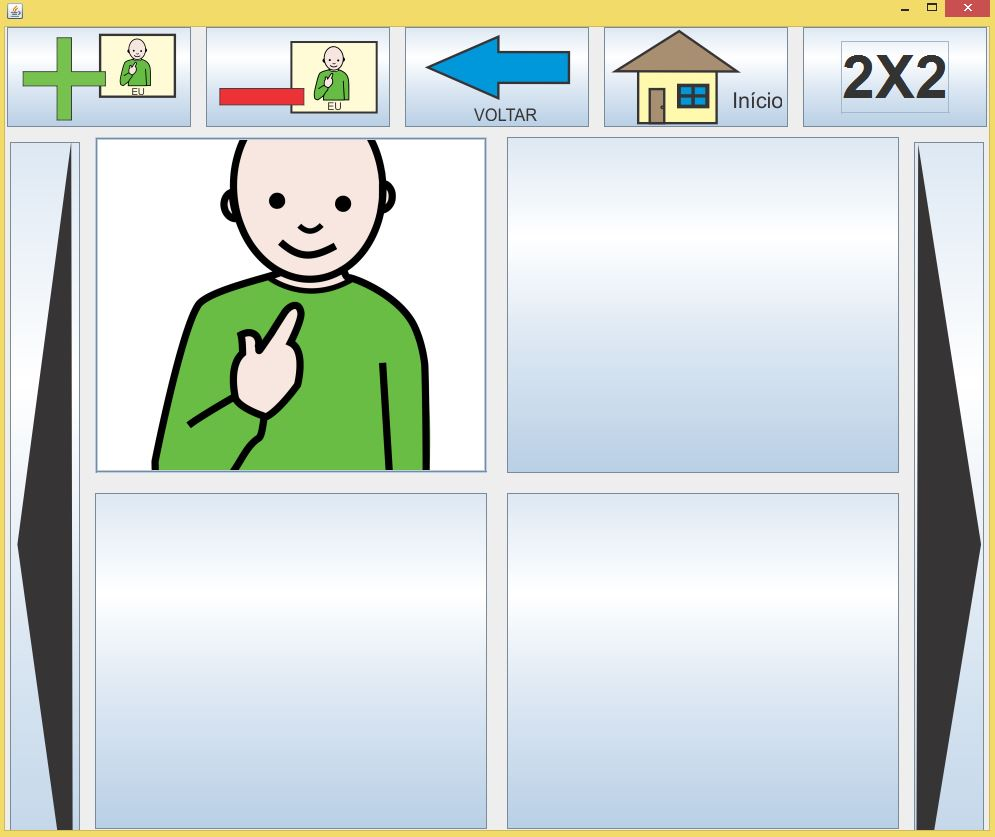
\includegraphics[width=10cm]{../figuras/solucao.jpg}\\
			Fonte:\cite{vivere}
    
    \label{fig:solucao}
  \end{center}
\end{figure}


Os �cones foram desenhados pelo autor, e cada um foi desenhado com o intuito de representar as a��es de uma maneira intuitiva, e baseados no desenho universal visando a acessibilidade. Al�m disso foi implementado uma nova funcionalidade a solu��o. � de senso comum na inform�tica que os �cones de um aplicativo, software ou ferramenta, sejam navegados atrav�s das teclas TAB e SHIFT+TAB do teclado. Por�m os dispositivos alternativos de teclado em sua maioria, como o que foi exemplificado no cap�tulo \ref{conceitos}n�o possuem essas teclas. Por esse motivo na solu��o a funcionalidade foi trocada para as teclas de seta para direita e seta para esquerda, e al�m disso o sombreado tradicional na tecla em que se encontra a navega��o foi substitu�da por vermelho, por ser considerada sutil pelo autor. Os conceitos de desenho universal tem como pressupostos\cite{desenho}:

\begin{itemize}
\item Equipara��o nas possibilidades de uso;
\item Flexibilidade no uso;
\item Uso simples e intuitivo;
\item Capta��o da informa��o;
\item Toler�ncia para o erro; e
\item Dimens�o e espa�o para uso e intera��o.
\end{itemize}


Ap�s a implementa��o da proposta foram realizados alguns testes, com os objetivos de:

\begin{enumerate}

\item Melhorar a usabilidade da solu��o;
\item Envolver usu�rios;
\item Observar usu�rios e suas a��es durante o uso da solu��o; e
\item Mensurar a��es permitindo o planejamento de mudan�as.

\end{enumerate}

\section{Testes}

Os testes foram divididos em duas etapas, afim de separar o experimento para dois p�blicos distintos.
O primeiro pessoas que possuem conhecimento focado em computa��o e a segunda com pessoas que possuem o conhecimento focado
na sa�de. O objetivo de separa-lo foi a tentativa de abranger as funcionalidades com vis�es distintas sobre a solu��o.


\section{Fase Um}

Na primeira fase os testes foram realizados com um grupo de 10 pessoas que atendem os requisitos mencionados na
no cap�tulo \ref{cap:proposta}. Os testes foram realizados em um ambiente controlado e com os mesmos equipamentos,
ap�s o usu�rio receber a tarefa, o usu�rio a realiza, e em seguida responde as perguntas do question�rio \ref{questionario}
relacionadas aquela tarefa. Ao final dos testes o usu�rio deixa um coment�rio sobre a aplica��o e seu funcionamento.
A tabela \ref{resultadosfaseum} representa os resultados obtidos na primeira fase dos testes. A tabela representa a m�dia obtida em cada pergunta para cada tarefa.

\begin{table}[bth!]
\centering
\scriptsize
\caption{Resultados da primeira fase dos testes.}\vspace{.2cm}

	
    \begin{tabular}{ | l | l | l | l | l |}
		
    \hline
    Atividades & Tarefa 1 & Tarefa 2 & Tarefa 3 & Tarefa 4\\ \hline \hline
    Qual foi o grau de dificuldade encontrado na realiza��o da tarefa? & 1,2 & 1,4 & 1,3 & 1,5\\ \hline
		Os passos da tarefa estavam claros? & 1,5 & 1,1 & 1,2 & 1\\ \hline
		Quantos erros foram cometidos na realiza��o da tarefa? & 0 & 0 & 0 & 0\\ \hline
		Ap�s a realiza��o da tarefa o objetivo foi cumprido? & 1 & 1 & 1.1 & 1\\ \hline
		
    \end{tabular}
    \label{resultadosfaseum}
		\vspace{0.1cm}\\Fonte: o pr�prio autor.

\end{table}

Nenhuma tarefa obteve resultados que infringissem o crit�rio de revis�o descrito no cap�tulo \ref{cap:proposta}. Por tanto a solu��o n�o passou por nenhuma revis�o antes dos testes passarem para a segunda fase dos testes.


\section{Fase Dois}


Na fase dois os testes foram realizados com pessoas que trabalham na �rea da sa�de, mais especificamente com pessoas que trabalham
com pessoas que possuem \ac{PC}. Nesta fase foram realizados os testes com 3 profissionais da sa�de, sendo um psic�logo, dois terapeutas ocupacionais. A tabela \ref{resultadosfasedois} representam os resultados do question�rio aplicados. 

\begin{table}[bth!]
\centering
\scriptsize
\caption{Resultados da segunda fase dos testes.}\vspace{.2cm}

	
    \begin{tabular}{ | l | l | l | l | l |}
		
    \hline
    Atividades & Tarefa 1 & Tarefa 2 & Tarefa 3 & Tarefa 4\\ \hline \hline
    Qual foi o grau de dificuldade encontrado na realiza��o da tarefa? & 1,34 & 1 & 1,34 & 1\\ \hline
		Os passos da tarefa estavam claros? & 1,67 & 1,34 & 1,34 & 1\\ \hline
		Quantos erros foram cometidos na realiza��o da tarefa? & 1 & 0 & 0 & 0\\ \hline
		Ap�s a realiza��o da tarefa o objetivo foi cumprido? & 1,67 & 1 & 1 & 1\\ \hline
		
    \end{tabular}
    \label{resultadosfasedois}
		\vspace{0.1cm}\\Fonte: o pr�prio autor.

\end{table}

Apesar de resultados semelhantes a primeira etapa, na Tarefa 1 (Executar um pictograma) infringiu o crit�rio de revis�o em duas perguntas. Foi encontrado que o termo grade inicial, mencionado nos passos para realiza��o da tarefa um, n�o foi compreendido. A altera��o na escrita dos passos foram alterados.


\section{Considera��es do Cap�tulo}

Os projetos definidos nos cap�tulos anteriores, foram fundamentais para a implementa��o da solu��o. Com o projeto definido
a implementa��o foi facilitada e possibilitou a implementa��o de uma nova funcionalidade. Os testes tamb�m foram igualmente importantes, pois demonstraram ao autor a rea��o das pessoas em rela��o as tarefas e interface.

\chapter{Considera��es Finais}
\label{cap:finais}

O objetivo do trabalho estipulado para o TCC-I e TCC-II foi parcialmente alcan�ado, a maneira utilizada para mensurar essa conclus�o, foi a do cumprimento de objetivos espec�ficos definidos previamente no plano do trabalho. Os objetivos espec�ficos podem ser citados atrav�s de dez etapas descritas no plano do trabalho:
\begin{enumerate}
\item Defini��o do Problema:
\begin{enumerate}
\item Contextualizar as necessidades do trabalho: que foi realizada atrav�s de pesquisa referenciada, descrita no cap�tulo \ref{cap:introducao}. Foram contextualizadas as necessidades de recursos que supram ou compensem suas defici�ncias para que possam ser inseridas na sociedade;
\item As regulamenta��es: s�o contextualizadas tamb�m no cap�tulo \ref{cap:introducao}, concluindo que o escopo do trabalho pertence a uma legisla��o recente e pouco espec�fica;
\item Limita��es: s�o mencionadas ao final do cap�tulo \ref{cap:introducao}, na qual o trabalho defini os quadros de pessoas portadoras de \ac{PC} que pertencer�o ao escopo do trabalho; e
\item Defini��o do problema: A defini��o do problema, contextualizado no cap�tulo {\ref{cap:definicao_problema}}, foi elaborada ap�s o levantamento dos problemas da solu��o utilizada por terapeutas, foi realizada atrav�s de uma entrevista\cite{juliane} com uma psic�loga especialista na reabilita��o de crian�as com \ac{PC}.
\end{enumerate}
\item Especifica��o de requisitos funcionais e n�o funcionais: A especifica��o dos requisitos foi elaborada a partir da defini��o do problema e dos problemas com a prancha de comunica��o utilizada por terapeutas e psic�logos definidas na se��o \ref{req} cap�tulo \ref{cap:definicao_problema};
\item Casos de uso: Os casos de uso definidos na se��o \ref{diagramas}, foram elaborados a partir da defini��o dos m�todos que s�o utilizados para o cumprimento dos requisitos. Os casos de uso tamb�m foram elaborados a partir de algumas diretrizes de usabilidade definidas na especifica��o da proposta;
\item Plano de testes: Os planos de testes foram definidos na se��o \ref{testes}, os planos foram divididos em etapas com a finalidade de quando chegar a �ltima etapa, que � a etapa realizada com usu�rios finais, a solu��o j� ter um amadurecimento maior para conseguir alcan�ar os objetivos esperados;
\item An�lise de alternativas: Foram feitas an�lises de alternativas para os principais problemas contextualizado na se��o \ref{esp}, comparando os m�todos encontrados com os requisitos para obter um m�todo que se suprisse os requisitos levantados;
\item Trabalhos Correlatos: Foi elaborado uma pesquisa para encontrar os trabalhos correlatos, e ap�s isso foram comparados com os requisitos levantados, a tabela \ref{tabela_correlatos} e \ref{tabela_correlatos} possibilitam comparar todos os requisitos com os trabalhos correlatos, e � poss�vel perceber que nem todos os requisitos s�o cumpridos por apenas um trabalho;
\item Projeto de Aplica��o;
\begin{enumerate}
\item Limita��es: as limita��es da solu��o proposta est�o atrelados aos m�todos de solu��o de requisitos definidos e consequentemente pela plataforma que executar� a execu��o; e 
\item Proposta: a proposta foi elaborada atrav�s de um prot�tipo de baixa fidelidade da solu��o e a defini��o das intera��es do usu�rio, atrav�s de diagramas de sequ�ncia, estado e representa��es de telas atrav�s de imagens.

\end{enumerate}
\item Implementa��o. Desenvolvimento da proposta de solu��o;
\item Testes. Consiste em verificar se o software proposto cumpre seu objetivo, testando e avaliando
os resultados; e
\item Escrita do TCC-II.
\end{enumerate}

As conclus�es e considera��es do trabalho certamente foram sobre as poucas op��es de ferramentas que psic�logos e terapeutas possuem a sua disposi��o para o trabalho com pessoas com \ac{PC}. A \ac{TA} por ser recente ainda n�o � muito conhecida e por consequ�ncia pouco utilizada. Com esses fatores a import�ncia de ressaltar as iniciativas e legisla��es, al�m de propor uma nova alternativa foram intensificadas. Outro fator que contribuiu com o cumprimento do objetivo foi a especifica��o detalhada da solu��o, e principalmente o entusiasmo das pessoas que foram apresentadas ao projeto. 

As principais dificuldades encontradas foram a forma correta de expor as ideias encontradas na literatura, com a finalidade de exemplificar as necessidades do trabalho. Outra dificuldade encontrada foi a elabora��o dos diagramas e telas dos sistema com o prop�sito de n�o deixar nenhuma d�vida quanto aos objetivos e prop�sitos da solu��o. Ainda em rela��o as dificuldades, o tempo de prepara��o de uma pessoa com paralisia cerebral para a realiza��o da terceira etapa dos testes, descritas no cap�tulos \ref{cap:proposta} segundo o pr�prio terapeuta, tornou invi�vel a documenta��o neste trabalho.

As atividades previstas no cronograma proposto no plano do trabalho at� o presente momento s�o:
\begin{enumerate}
\item{Formula��o do plano de TCC;}
\item{Levantamento e fichamento de refer�ncias. Consiste na pesquisa de
fontes para cada objetivo espec�fico citado na segunda se��o;}
\item{Consolida��o das refer�ncias. Fornece a fundamenta��o necess�ria para
poder compreender o objeto do trabalho e realizar o objetivo do TCC-I;}
\item{An�lise. Analisar pontos espec�ficos levantados na pesquisa referencial;}
\item{Escrita do TCC-I;}
\item{Apresenta��o da proposta do software. Consiste em apresentar propostas de solu��o e justificar a proposta
escolhida;}
\item{Revis�o de conceitos no projeto do software. Fundamenta��o necess�ria
para execu��o do projeto;}
\item {Implementa��o. Desenvolvimento da proposta de solu��o;}
\item {Testes. Consiste em verificar se o software proposto cumpre seu objetivo, testando e avaliando
os resultados; e}
\item {Escrita do TCC-II.}
\end{enumerate}

A tabela \ref{etapas} representa a conclus�o das tarefas de acordo com os meses do ano de 2014:

\vspace{3.0cm}
\begin{table}[bth!]
\begin{center}
\scriptsize
\caption{Tabela de conclus�o das tarefas do TCC-I e II.}
\vspace{0.3cm}
 \begin{tabular}{|c||c|c|c|c|c|c|c|c|c|c|c|c| }
  \hline
  \multirow{2}{*}{\textbf{\small{Etapas}}} & \multicolumn{12}{|c||}{\textbf{\small{2014}}}  \\
  \cline{2-13}
   & \textbf{J} & \textbf{F} & \textbf{M} & \textbf{A} & \textbf{M} & \textbf{J} & \textbf{J} & \textbf{A} & \textbf{S} & \textbf{O} & \textbf{N} & \textbf{D}  \\
  \hline \hline
  \textbf{\small{1}} & &X & & & & & & & & & & \\
  \hline
  \textbf{\small{2}} & &X&X& & & & & & & & & \\
  \hline
  \textbf{\small{3}} & & &X& & & & & & & & &  \\
  \hline
  \textbf{\small{4}} & & &X&X& & & & & & & &  \\
  \hline
  \textbf{\small{5}} & & &X&X&X&X& & & & & &  \\
  \hline
  \textbf{\small{6}} & & & & &X&X&& & & & &  \\
  \hline
  \textbf{\small{7}} & & & & & &X& & & & & &  \\
	\hline
	\textbf{\small{8}} & & & & & & X & X& X& & & & \\
  \hline
  \textbf{\small{9}} & & & & & & & & X& X & & & \\
  \hline
  \textbf{\small{10}} & & & & & & & & &X &X &X &  \\
	\hline
\end{tabular}
\label{etapas}
\end{center}
\end{table}

A tabela \ref{etapas} representa o cronograma do trabalho cumprido at� o momento. Os per�odos de execu��o das tarefas diferem dos apresentados no plano do trabalho, por falta de experi�ncia e de planejamento do autor. Cumpridas as tarefas descritas para o TCC-I e II. Para trabalho futuros, s�o indicados a continua��o dos testes que n�o foram poss�veis a realiza��o, j� firmados com o Grupo Assistiva da UDESC e a implanta��o e testes da solu��o em outras plataformas.

      %chamada de arquivo capitulos.tex (desenvolvimento de seu TCC efetivamente)

\chapter{Conclus�es}
\label{cha:conclusao}
      %chamada de arquivo conclusao.tex 
%--------------Bibliografia e ap�ndices--------------------
\bibliographystyle{abnt-alf}
\bibliography{../4_pos_texto/bibliografia}     %chamada de arquivo bibliografia.bib
\anexo
\chapter{Primeiro anexo}

 Anexos s�o documentos n�o elaborados pelo autor, que servem de fundamenta��o, comprova��o ou ilustra��o.

		       %chamada de arquivo anexo.tex
\appendix
\chapter{Ap�ndice}
\renewcommand{\thesection}{\Alph{section}}
\section{Quadros Cl�nicos de Paralisia Cerebral}
\label{apendice1}
\begin{enumerate}
\item {Hemiplegia : � a manifesta��o mais frequente, com
maior comprometimento do membro superior;
acompanha-se de sinais de libera��o tais como
espasticidade , hiper reflexia e sinal de Babinski. O
paciente assume atitude em semiflex�o do membro
superior, permanecendo o membro inferior
hiperestendido e aduzido, e o p� em postura equinovara.
� comum hipotrofia dos segmentos acometidos, sendo
tamb�m poss�vel a ocorr�ncia de outras hemi-hipoestesia
ou hemianopsia.}
\item{ Hemiplegia bilateral ( tetra ou quadriplegia) :
Ocorrem de 9 a 43\% dos pacientes. Ocorrem les�es
difusas bilateral no sistema piramidal dando al�m da
grave tetraparesia esp�stica com intensas retra��es em
semiflex�o, s�ndrome pseudobulbar (hipomimia, disfagia
e disartria), podendo ocorrer ainda microcefalia,
defici�ncia mental e epilepsia.}
\item{Diplegia : Ocorre em 10 a 30 \% dos pacientes, sendo
a forma mais encontrada em prematuros. Tratase de um
comprometimento dos membros inferiores, comumente
evidenciando uma acentuada hipertonia dos adutores,
que configura em alguns doentes o aspecto semiol�gico
denominado s�ndrome de Little (postura com cruzamento
dos membros inferiores e marcha em tesoura). H� 
diferentes grada��es quanto � intensidade do dist�rbio,
podendo ser pouco afetado (tendo recupera��o e bom
progn�stico  adaptam-se � vida di�ria); enquanto outros
evoluem mal com graves limita��es funcionais. Os dados
semiol�gicos s�o muito vari�veis. No 1� ano de vida, a
crian�a apresenta-se hipot�nica, evoluindo
gradativamente para uma outra fase em que se observa
um quadro de distonia intermitente, com tend�ncia ao
opist�tono quando estimulada. Nos casos mais graves a
crian�a pode permanecer num destes est�gios por toda
a sua vida, por�m geralmente passa a exibir hipertonia
esp�stica, inicialmente extensora e, finalmente, com
graves retra��es semiflexoras.}
\item{Discinesia : Atualmente � a mais rara, pois
manifesta-se atrav�s de movimentos involunt�rios,
sobretudo distonias axiais e/ou movimentos c�reoatet�ides
das extremidades. No primeiro ano de vida este
padr�o costuma n�o estar definido, podendo existir
hipotonia muscular. Em geral, quando estes pacientes
est�o relaxados a movimenta��o passiva � facilitada.}
\item{Ataxia : Igualmente rara. Inicialmente pode traduzir se
por hipotonia e, aos poucos, verificam-se altera��es
do equil�brio (ataxia axial) e, menos comumente, da
coordena��o ( ataxia apendicular). Sua marcha se faz com
aumento da base de sustenta��o podendo apresentar
tremor intencional.}
\item{Formas mistas : � a associa��o das manifesta��es
anteriores, correspondendo, geralmente, ao encontro de
movimentos dist�nicos e c�reo atet�ides ou �
combina��o de ataxia com plegia (sobretudo diplegia).
No total, cerca de 75\% dos pacientes doentes com
paralisia cerebral apresentam padr�o esp�stico.
Al�m do dist�rbio motor, obrigat�rio para a
caracteriza��o da paralisia cerebral, o quadro cl�nico pode
incluir tamb�m outras manifesta��es acess�rias com
frequ�ncia vari�vel: 
\begin{enumerate}
\item{ Defici�ncia mental: Ocorre de 30 a
70\% dos pacientes. Est� mais associada �s formas
tetrapl�gicas, dipl�gicas ou mistas;}
\item{ Epilepsia: Varia de
25 a 35\% dos casos, ocorrendo mais associado com a
forma hemipl�gica ou tetrapl�gica; }
\item{ Dist�rbios da
linguagem; }
\item{ Dist�rbios visuais : Pode ocorrer perda da
acuidade visual ou dos movimentos oculares
\(estrabismo\); }
\item{ Dist�rbios do comportamento : S�o mais
comuns nas crian�as com intelig�ncia normal ou lim�trofe,
que se sentem frustradas pela sua limita��o motora,
quadro agravado em alguns casos pela super prote��o
ou rejei��o familiar; e}
\item{ Dist�rbios ortop�dicos : Mesmo
nos pacientes submetidos � reabilita��o bem orientada,
s�o comuns retra��es fibrotend�neas \(50\%\) cifoescoliose
\(15\%\), coxa valga \(5\%\) e deformidades nos p�s.
Todos esses dist�rbios se d�o devido a altera��es
nas �reas motoras cerebrais espec�ficas durante a
inf�ncia.}
\end{enumerate}
}
\end{enumerate}
\newpage
\section{Entrevista}
\label{entrevista}
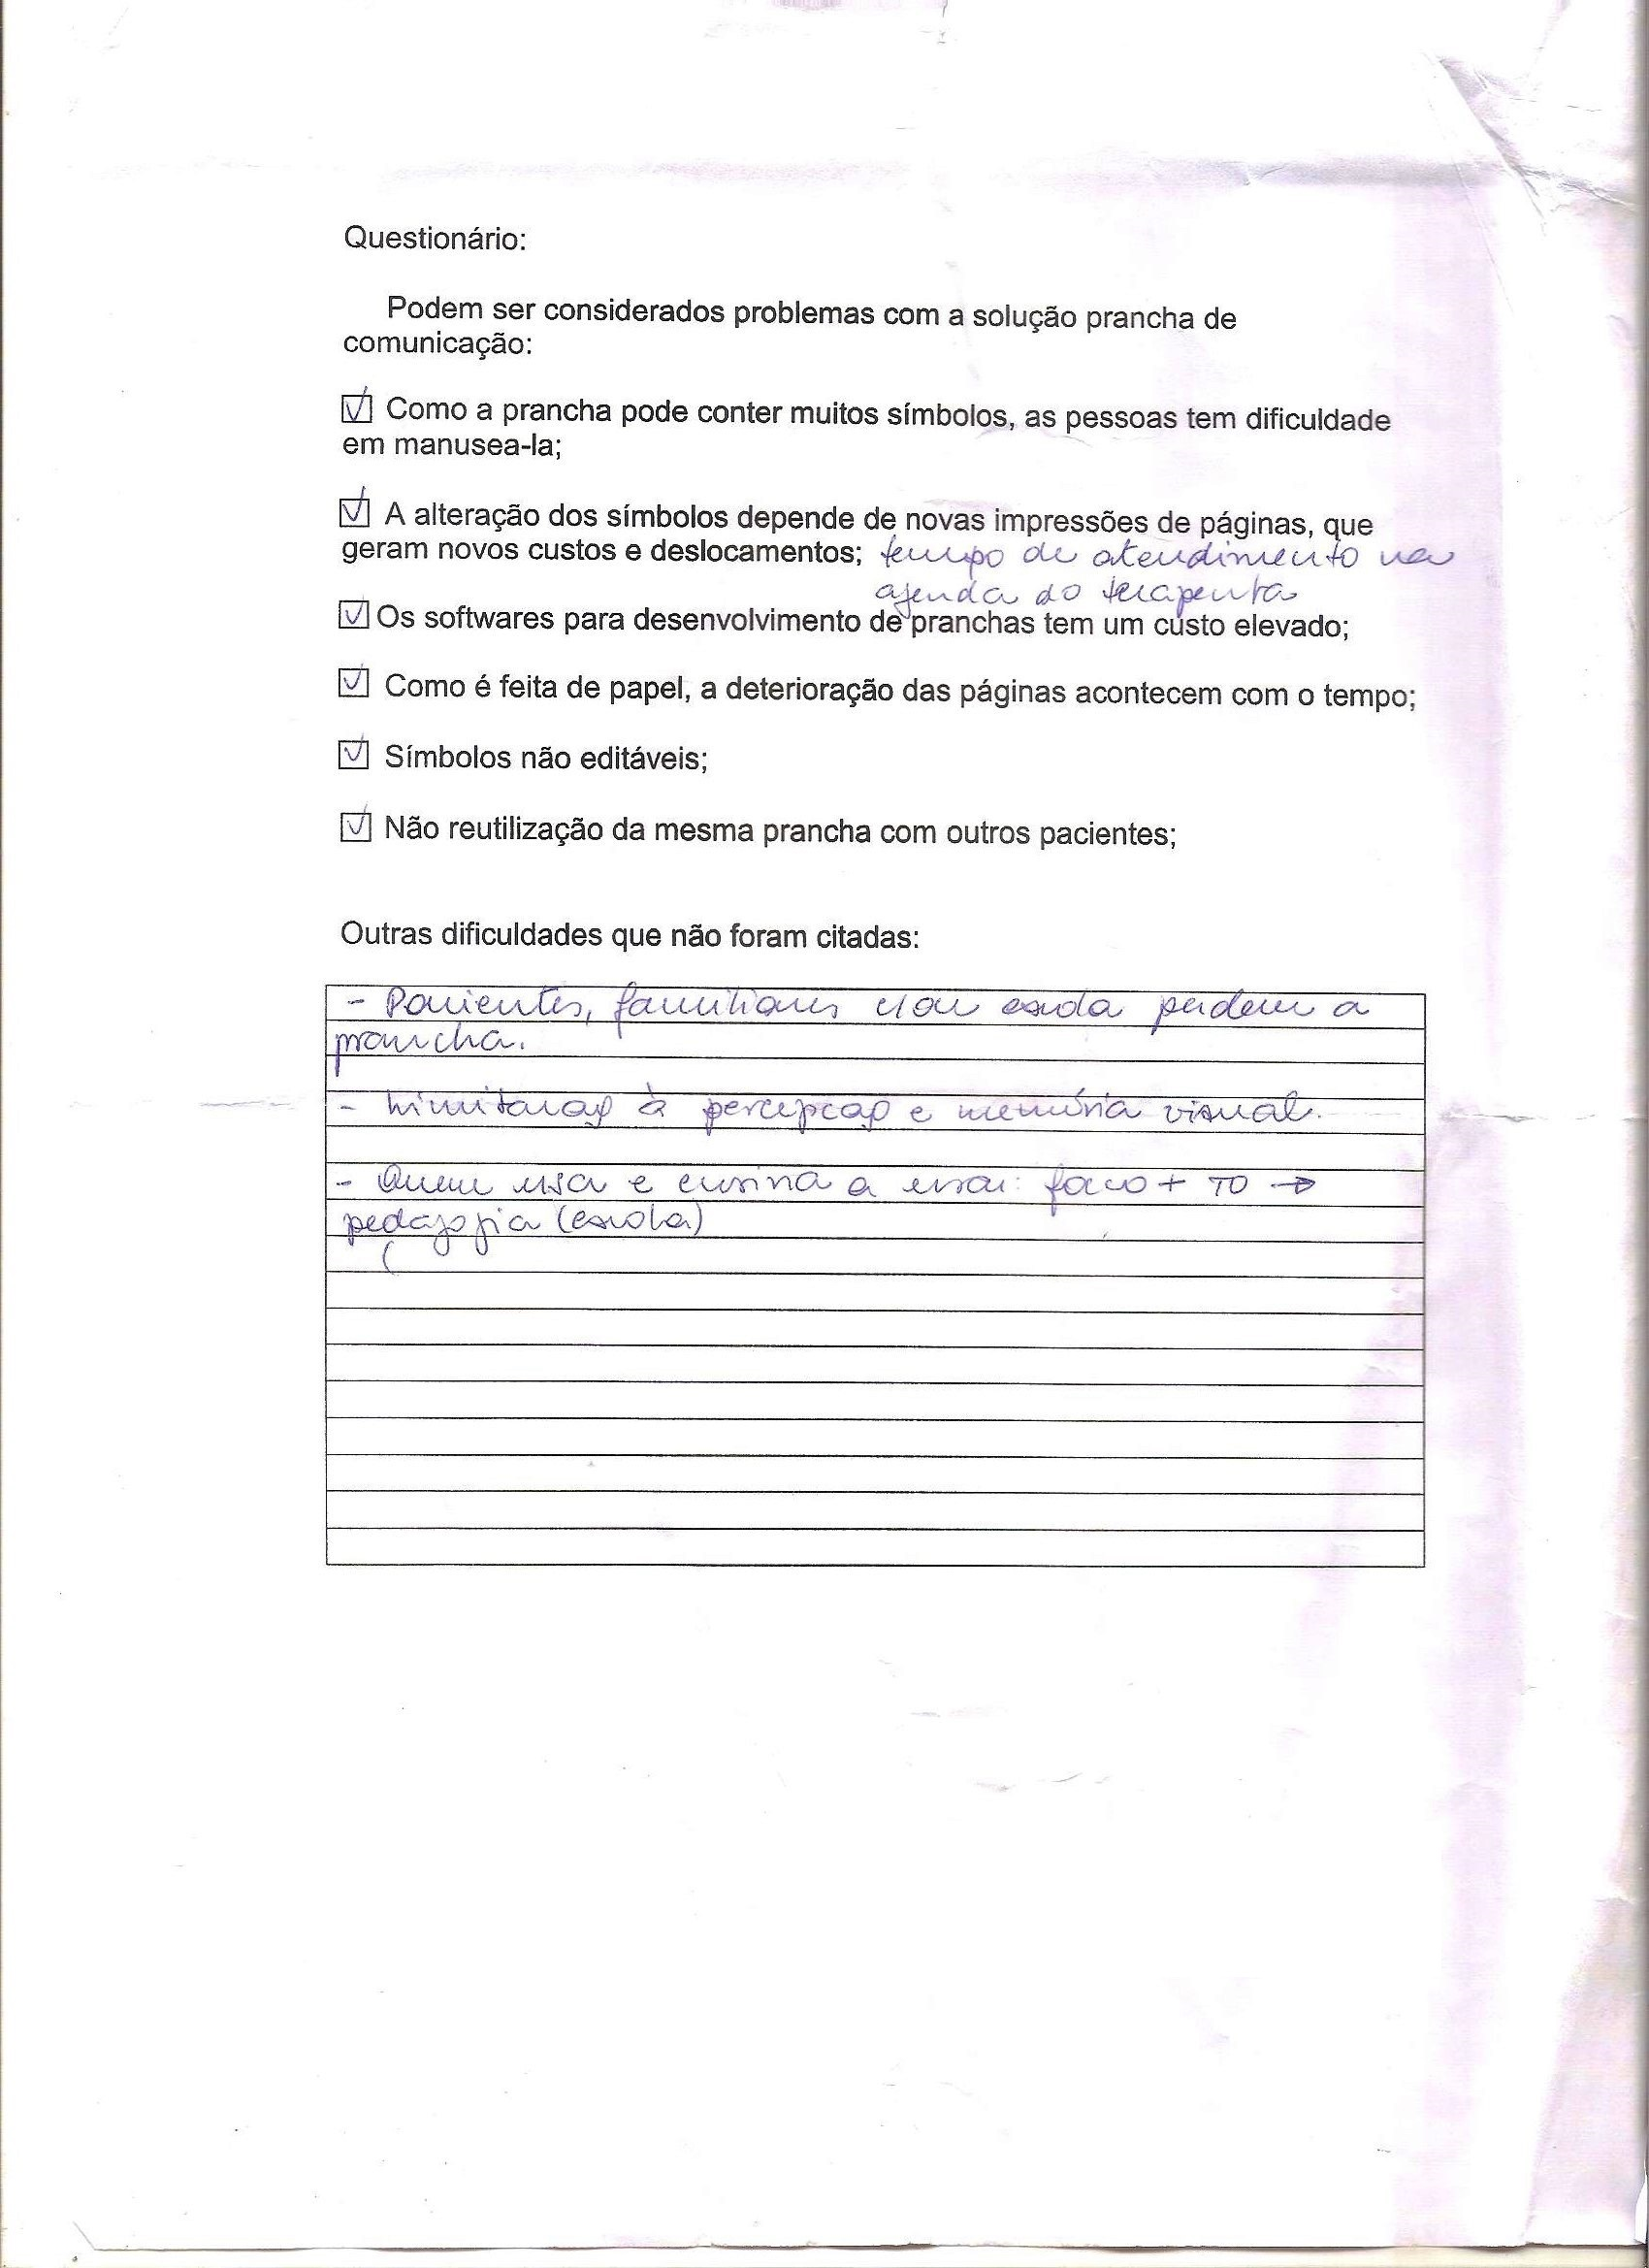
\includegraphics[scale=0.8]{../figuras/entrevista.jpg}
	               %chamada de arquivo apendice.tex
\end{document}